\documentclass[refcompress,eversion,noinfo]{XDUthesis}
% 正文大约需要60页
\usepackage{multirow}
\usepackage{graphicx}
\usepackage{diagbox}
\usepackage[subrefformat=parens,labelformat=parens]{subfig}
\usepackage{caption}
\usepackage{tikz}
\usepackage{color}
\usepackage{verbatim}
\usetikzlibrary{positioning} % L ATEX and plain TEX
\usepackage{amsmath}
\usepackage[chapter]{algorithm}
\usepackage{algorithmic}

% 不生成PDF
%\usepackage{syntonly}
%\syntaxonly

% 生成目录
\usepackage[chapter, nottoc]{tocbibind}

% http://tex.stackexchange.com/questions/198140/glossaries-and-custom-section-headings-broken  \glsentrytext!
\usepackage[nomain,acronym,xindy,toc,nopostdot]{glossaries}
\makeglossaries
\usepackage{booktabs}
\graphicspath{{figures/}}


% my command
\newcommand{\firstgls}[1]{\textbf{\,\gls{#1}}(\glsdesc{#1})}
\newcommand{\firstacr}[1]{\textbf{\,\gls{#1}}(\glssymbol{#1})}
\newcommand{\glsacr}[1]{\gls{#1}(\glssymbol{#1})}
\newcommand{\firstall}[1]{\textbf{\,\gls{#1}}(\glsdesc{#1}, \glssymbol{#1})}
\newcommand{\ENNAME}[1]{\text{#1}}
\newcommand{\NUMTEXT}[1]{\text{#1}}
\newcommand{\figref}[1]{图\,\ref{#1}\,}
\newcommand{\chapref}[1]{第\ref{#1}章}
\newcommand{\secref}[1]{第\,\ref{#1}\,节}
\newcommand{\algref}[1]{算法\,\ref{#1}\,}
\newcommand{\eqnref}[1]{式\,\eqref{#1}\,}


\begin{document}
\XDUfrontmatter

\begin{abstract}
复杂电磁环境下的无线信号认知是优化频谱利用、识别和最小化干扰,并实施行为策略和有效协调系统的重要工具。传统方法的研究主要集中在能量检测以及专家特征和决策准则的使用,以获取对不同信号的认知能力。这些方法依赖于信号属性、特征和决策统计的先验知识来分离已知的信号(如调制)类型,并且通常在简化的硬件资源、低干扰无线传播环境模型下得到。\par

随着深度学习发展,利用原始采样信号进行特征学习并对(调制)信号分类得以实现;并且,在灵敏度和准确性方面优于传统的基于专家特征提取进行统计分类决策。这为当前的无线信号识别的相关问题提供了一种全新的解决方案,但它仍然完全依赖于监督学习。在现实世界中,特别是在无线电领域,我们面临着大量的未标记的示例数据,我们的传感器感知的也只是小部分的标签数据以及大部分的无标签数据,只能获取目标的不完整低可靠性的知识。\par

无线信号数据易于从天线获得,但有类别标记信号样本数据通常很少,若直接使用传统的监督学习技术,仅能使用有标记数据构建模型,而无法利用未标记的数据来学习信号所包含的信息;同样由于有标记的样本信号较少,训练样本不足,学习泛化能力较差。因此,我们可以利用半监督学习技术,结合深度学习技术,进行有效的无线信号感知\par

在复杂电磁环境下,完成不同信噪比、不同专家特征集条件下,利用无监督数据构建原始信号的征稀疏表示;针对无线信号应用场景,融合专家指纹特征与深度网络特征,利用监督数据构建无线信号的完备特征集,建立无线信号调制方式分类器,完成已知信号的调制方式识别;针对低信噪比条件,分析不同网络结构对于信号分类结果的影响,构建特征融合的最优分类器。\par

第三章 提出了一种CAE-CNN调制识别的算法框架。
首先,介绍了调制信号的生成;
然后,对信号进行了时频域可视化,利用监督方法和无监督方法将信号特征可视化;
接下来,我们将监督方法与无监督方法融合,提出了CAE-CNN的算法;
最后,我们将所提算法的性能进行展示并与传统的方法进行比较。 \par

第四章 提出了一种传统特征与深度特征融合的框架。
首先,介绍了常用的调制识别所用的特征;
然后,对特征融合的相关理论进行概述;接
着,提出了基于LR、DNN以及集成树的融合框架;
最后,对不同特征融合算法的仿真结果进行了相应的理论分析。 \par

第五章 对调制识别的不同网络结构进行了分析验证。
首先,基于CNN网路框架,研究了卷积核数目、大小以及卷基层深度对调制识别的影响;
接下来,研究了网络底层结构(如CLDNN、ResNet等)对调制识别的影响,并对仿真结果进行了理论分析。\par

利用深度网络对无线信号进行特征学习,可以获得更能表征信号原始特征的稀疏特征空间。将传统无线信号特征与深度学习特征相融合,构建信号的完备特征集,并将其作为分类的特征空间。首先,对深度网络进行预训练,获取可以表征信号的深度特征空间;进而,将传统特征进行归一化等一系列的预处理,作为新的特征并以全连接的形式输入到分类器;这样整个分类器的输入特征空间相当于深度特征与传统特征的结合,在保证分类准确率的条件下,能够兼顾传统特征与深度特征,充分利用传统方法所获取的先验知识。在特征融合之后,利用监督数据对于整个网络进行训练,以获取最优分类网络。\par

\keywords{XXX,\quad{}XXX,\quad{}XXX,\quad{}XXX,\quad{}XXX} \\
\end{abstract}

\begin{englishabstract}
The Abstract is a brief description of a thesis or dissertation without notes or comments. It represents concisely the research purpose, content, method, result and conclusion of the thesis or dissertation with emphasis on its innovative findings and perspectives. The Abstract Part consists of both the Chinese abstract and the English abstract. The Chinese abstract should have the length of approximately 1000 Chinese characters for a master thesis and 1500 for a Ph.D. dissertation. The English abstract should be consistent with the Chinese one in content. The keywords of a thesis or dissertation should be listed below the main body of the abstract, separated by commas and a space. The number of the keywords is typically 3 to 5.
\\~\\
The format of the Chinese Abstract is what follows: Song Ti, Small 4, justified, 2 characters indented in the first line, line spacing at a fixed value of 20 pounds, and paragraph spacing section at 0 pound.
\\~\\
The format of the English Abstract is what follows: Times New Roman, Small 4, justified, not indented in the first line, line spacing at a fixed value of 20 pounds, and paragraph spacing section at 0 pound with a blank line between paragraphs.
~\\
\englishkeywords{XXX,\space{}XXX,\space{}XXX,\space{}XXX,\space{}XXX} \\

\end{englishabstract}


\XDUpremainmatter

\begin{symbollist}
\item [符号] \hspace{12em} {符号名称}
\item [$\in$]\hspace{12.5em} {属于}
\item [$\mathbb{R}$]\hspace{12.5em} {实数集}
\item [$w$] \hspace{12.5em} {权重}
\item [$x$] \hspace{12.5em} {样本}
\item [$y$] \hspace{12.5em} {标签}
\item [$M$] \hspace{12.5em} {特征维数}
\item [$N$] \hspace{12.5em} {样本数量}
\item [$\eta$] \hspace{12.5em} {学习率}
\item [$\mathcal{F}^{-1}$] \hspace{12.5em} {逆傅里叶变换}
\item [$\gamma$] \hspace{12.5em} {弱分类器更新率}
\end{symbollist}

\begin{abbreviationlist}
\item \makebox[8em][l]{缩略语}  \makebox[16em][l]{英文全称}  \makebox[16em][l]{中文对照}
\item \makebox[4em][l]{SVM}    \makebox[20em][l]{Support Vector Machine}    \makebox[16em][l]{支持向量机}
\item \makebox[4em][l]{EM}    \makebox[20em][l]{expectation–maximization}    \makebox[16em][l]{最大期望}
\item \makebox[4em][l]{WTS}   \makebox[20em][l]{Weighted Tensor Subspace}    \makebox[16em][l]{加权张量子空间}
\item \makebox[4em][l]{PCA}    \makebox[20em][l]{Principal Component Analysis}    \makebox[16em][l]{主成分分析}
\item \makebox[4em][l]{IPCA}    \makebox[20em][l]{Incremental PCA}    \makebox[16em][l]{增量主成分分析}
\item \makebox[4em][l]{HOG}    \makebox[20em][l]{Histogram of Oriented Gradient}    \makebox[16em][l]{方向梯度直方图}
\item \makebox[4em][l]{2D-LDA}    \makebox[20em][l]{2D Fisher Linear Discriminant Analysis}  \makebox[16em][l]{二维Fisher线性判别分析}
\item \makebox[4em][l]{AVT}    \makebox[20em][l]{Attentional Visual Tracking}    \makebox[16em][l]{注意视觉跟踪}
\item \makebox[4em][l]{RF}    \makebox[20em][l]{Random Forest}    \makebox[16em][l]{随机森林}
\item \makebox[4em][l]{FFT}    \makebox[20em][l]{Fast Fourier Transformation}    \makebox[16em][l]{快速傅里叶变换}
\item \makebox[4em][l]{MOSSE}   \makebox[20em][l]{Minimum Output Sum of Squared Error filter}    \makebox[10em][l]{最小平方误差滤波器}
\item \makebox[4em][l]{CFT}    \makebox[20em][l]{Correlation Filter Tracker}    \makebox[16em][l]{相关滤波跟踪器}
\item \makebox[4em][l]{DFT}    \makebox[20em][l]{Discrete Fourier Transform}    \makebox[16em][l]{离散傅里叶变换}
\item \makebox[4em][l]{KCF}    \makebox[20em][l]{Kernelized Correlation Filter}    \makebox[16em][l]{核相关滤波器}
\item \makebox[4em][l]{CLE}    \makebox[20em][l]{Center Location Error}    \makebox[16em][l]{中心位置误差}
\item \makebox[4em][l]{OP}    \makebox[20em][l]{Overlap Precision}    \makebox[16em][l]{重叠精度}
\item \makebox[4em][l]{DP}    \makebox[20em][l]{Distance Precision}    \makebox[16em][l]{距离精度}
\item \makebox[4em][l]{ASMM}    \makebox[20em][l]{Atkinson–Shiffrin Memory Model}    \makebox[16em][l]{AtkinsonShiffrin 内存模型}
\item \makebox[4em][l]{MUSTer}    \makebox[20em][l]{MUlti-Store Tracker}    \makebox[16em][l]{多贮存跟踪器}
\item \makebox[4em][l]{KNN}    \makebox[20em][l]{K-Nearest Neighbor}    \makebox[16em][l]{K-最近邻}
\item \makebox[4em][l]{HOG}    \makebox[20em][l]{Histogram of Oriented Gradient}    \makebox[16em][l]{方向梯度直方图}
\item \makebox[4em][l]{ALM}    \makebox[20em][l]{Augmented Lagrange Method}    \makebox[16em][l]{增强拉格朗日方法}
\item \makebox[4em][l]{ADMM}    \makebox[20em][l]{Alternating Direction Method of Multipliers}    \makebox[16em][l]{交替方向乘子算法}
\end{abbreviationlist}


\XDUmainmatter
\chapter{绪论}
\section{研究背景及研究意义}

\subsection{研究背景}
通信的主要目的是传递信息。 
无论是在传统的有线通信系统还是在无线通信系统中,由于信道传输特性的限制,
基带信号不能直接通过信道传输,而是需要对基带信号进行调制以将其搬移到 一定的频段进行有效地传输\cite{昌信2006通信原理}。 
同时,对基带信号的调制,还可以使通信系统在具有更高的传输速率的同时,提高频谱利用率。\par

随着通信技术的不断发展,终端的数目呈爆发性增长,用户对信息传输速率和传输稳定性的要求不断提高。
为了满足这样的需求,通信信号的调制形式由简单到复杂,调制方式由传统的模拟调制发展到主流的数字调制方式,
信道从有线信道到有线与无线信道混合组网。
调制是指将发送的信号加载到高频(基带调制除外)信号以适应信道传播环境的一种技术。
调制方式自动识别,是指在未给定调制信号所携信息的情况下,利用学习的算法,
通过接收信号电磁特性判定信号的调制方式。
模拟调制针对的是模拟信号,传统的模拟调制按照调制方式的不同,
可以分为幅度调制(AM)、频率调制(FM)和相位调制(PM)等;
数字调制针对的是数字信号,按照调制方式的不同可以分为
幅移键控(ASK)、频移键控(FSK)、相移键控(PSK)和正交幅度调制(QAM)等。 \par

调制信号的自动识别,是一种优化频谱利用效率,识别和最小化干扰,以及有效推动认知无线网发展的重要手段,
在协作通信和非协作通信中都得到了广泛应用\cite{nandi1995automatic}。
在军事领域,调制识别被广泛地用作通信侦察,电子战和威胁分析,是一种智能信号分析和处理的关键技术\cite{程汉文2009基于累计量的干扰信号调制识别算法}\cite{张春磊2013认知电子战初探}。
在侦听接收机的设计中,获取无线接收信号的调制方式是侦听接收机的重要功能之一。
有效的无线信号调制方式识别为解调器正确选择解调算法提供了参数依据,可以使我们最终得到准确的情报信息。
调制识别技术也有助于为电子战选择最佳的干扰模式或干扰消除算法,以保证我方设备之间通信的稳定性;
同时抑制和干扰对方的通信以达到电子战通信对抗的目的。\par

因此,通信信号调制自动识别技术具有非常广阔的应用前景,将成为未来的民用无线通信以及军事通信中的重要组成部分。\par

深度学习(Deep Learning,DL),是一种机器学习(Machine Learning,ML)领域的分支。
2006年Hinton等人提出了深度置信网络(Deep Belief Network, DBN)\cite{hinton2006fast},并引入了分层预训练技术,自此深度学习得到了广泛的应用。
在目标检测、语音识别、机器翻译等许多不同的人工智能任务中,深度学习已经极大地提升了这些任务上的最佳表现水平\cite{lecun2015deep}。 \par

2012年的ILSVRC2012竞赛中,Krizhevsky等人引入了Dropout等方法,训练了一个大型的深度卷积神经网络AlexNet,
使用深度学习模型击败了Google团队并取得了该竞赛的冠军,
使得图片识别错误率下降了$14\%$\cite{krizhevsky2012imagenet}。
2014年Christian Szegedy等人提出GoogLeNet,打破了常规的卷积层串联的模式,
将$1 \times 1, 3 \times 3, 5 \times 5$的卷积层和$3 \times 3$的池化层并联组合到一起,
以较大优势取得ILSVRC2014冠军并使top-5的错误率降到了$6.67\%$\cite{Szegedy_2015_CVPR}。
2015年,KaimingHe等人设计了一个多达152层的ResNet架构,
使图片识别的错误率也降到了$3.6\%$\cite{he2016deep}。
研究者在将深度学习应用到目标检测、面部识别或语言模型等传统任务的同时,
也在将其扩展到许多不同的现代领域和任务中,
比如Osako等人使用循环神经网络来给语音信号降噪\cite{osako2015complex},
Gupta等人使用堆栈自编码器(stacked autoencoders)来发现基因表达的聚类模式\cite{gupta2015learning},
Gatys等人使用一种神经模型来生成不同风格的图像\cite{gatys2015neural}等等。
深度学习在很多领域都取得了较大的发展。\par

\subsection{研究意义}

在无线通信中,调制识别是正确实现无线通信解调和保证正常接收的重要组成部分。
基带信号通常是频率非常低且分量很多的频谱,这些含有很多低频分量的信号不适合在信道中直接传输,
这就需要我们对基带信号进行调制,以适应信道的特性并在无线信道中进行有效传输。
信号在经过调制并通过信道到达接收端,与原始的信号具有很大的不同。
所以,只有在接收端确定信号的调制方式,才能利用相应的解调方法解调获取原始信息。
基于深度学习的调制识别的意义主要体现在以下几方面:\par

(1) 提高通信设备的稳定性与通用性,降低建设与运维成本。
通信技术的迅速发展导致了各种通信系统的共存,而这些通信系统的调制方式可能各不相同。
由于解调需要与调制进行匹配才能准确地接收发射信号,这些差异性的调制技术也导致接收机类型大幅增加。
于是,人们希望能够通过发展新的无线认知技术,基于通用的接收机平台来接收并识别不同的调制信号,
以减少接收机类型的快速增长。 \par

(2) 军事领域的电子对抗、电磁干扰与反干扰的基础。
当检测到对方无线电信号或电磁信号时,
需要我们对检测到的信号或电磁信息,进行调制识别以及载玻频率与波特率等参数的正确估计,
方便接下来的情报获取或者进行电磁干扰。\par

(3) 有助于如何在频域、时域和空域等多维度上有效分配频谱资源,提高频谱利用率。
在认知无线领域,无线频谱资源根据具体业务的不同,
主要划分为民用的广播电视、无线通信、卫星通信及军用的雷达与军事通信等不同频段。
为了避免相邻频段或频道的互相干扰,不同的通信业务的工作频段相互隔离,
并且不同频段之间预留一定的间隔频带;
上下频段的频谱资源分配以及频谱利用率极不平衡,造成了频谱资源的极大浪费。
由于无线频谱资源有限,随着频谱资源的消耗殆尽,
现有的频谱分配与管理机制已经成为制约无线通信进一步发展的重要因素。\par

(4) 利用深度学习的方法提升传统调制识别算法的性能上限。
在通信系统中使用DL有很多优点。 首先,由于通信基础设备以及终端的数量多,且通信数据速率高,因此可以很容易获取DL训练所需要的大量数据。
其次,DL可以自主提取特征,避免了手动特征选择这一繁琐且具有挑战性的任务。
另外,新的、更复杂的信号和通信应用的出现,给认知无线带来了更大的挑战;
有时,我们需要对一些未知的信号进行认知,而传统的基于特征的方法在新的场景下很难适应信号特性的变化。
因此,我们可以利用深度学习的特征自提取能力,来增强对于未知信号的认知能力。\par

(5) 促进深度学习在通信领域的发展。
在调制识别领域中,利用专家特征和判决准则进行调制识别得到了广泛的应用,
并且在特定情况下可以实现很高的识别准确率。
深度学习在计算机视觉和自然语言处理等领域的应用,绝大多数是基于数据进行特征与模型的学习,
而不是利用专家知识提取特征进而训练模型,这与很多传统的机器学习算法(比如DNN、SVM、决策树等)在算法思想上有很大不同。
而且,这些基于数据的深度学习算法在相应的领域取得了最好的性能。
因此,这就需要我们重新审视一下,是否也应该对通信领域的传统算法在思想上进行改变,
基于数据去理解信号,去学习信号本身的特征。\par

\section{无线信号调制识别的发展和研究现状}

早期调制识别的任务是由操作人员在仪器的帮助下完成的:
主要是通过观察和分析接收信号的时域波形和频谱形状,判断信号的调制方式,然后选择相应的解调器进行解调。
然而,随着无线通信技术尤其是数字通信技术的快速发展,信号调制方式变得越来越复杂,很难通过人工的方法来准确判别调制方式的类别。 
C.S.Waver等人1969年在斯坦福大学发表了第一篇关于通信信号调制识别的论文\cite{weaver1969automatic},
此后,调制方式的自动识别引起了人们的广泛关注,各种技术出版物上出现了许多关于调制识别的文章,
其中许多结果已经被应用到实际工作中。 \par

对于无线信号调制识别的研究,现有算法大致可以分为:基于假设检验的最大似然法,
基于特征提取的模式识别方法,以及基于深度学习的调制识别方法。
大多数基于假设检验的最大似然类方法计算复杂度较高,对模型失配问题较为敏感,这大大限制了它们在实际通信环境中的应用。
基于特征提取的模式识别方法,通常关注能量在不同频段上的分布,并使用专家特征和判别准则来识别和区分特定的调制方式。
在特定的条件下,基于特征的方法可以实现接近理论最佳的识别性能,并且其具备较强的鲁棒性,
因此得到更广泛的应用。
鉴于深度学习在其他领域取得的成果,深度学习可以与硬件结合自适地进行学习提高传统算法的性能上限,
并可以通过特定的正则化方法来降低过拟合提高模型的鲁棒性。
因此,深度学习在通信领域近年来已经成为一个研究热点,在调制识别领域也有很多人投入到相应的研究中。\par

\subsection{基于似然比判决理论的方法}

基于似然比决策理论的方法也叫做最大似然假设检验法。 
其基本思想是使用概率论和假设检验理论来分析信号的统计特性,
并依据损失函数最小化原则获取足够的统计信息,定义判决准则,对信号进行分类。
基于似然比判决理论的调制识别系统框图如图\ref{sec:fig_1_0}所示。\par

\begin{figure}
	\centering
	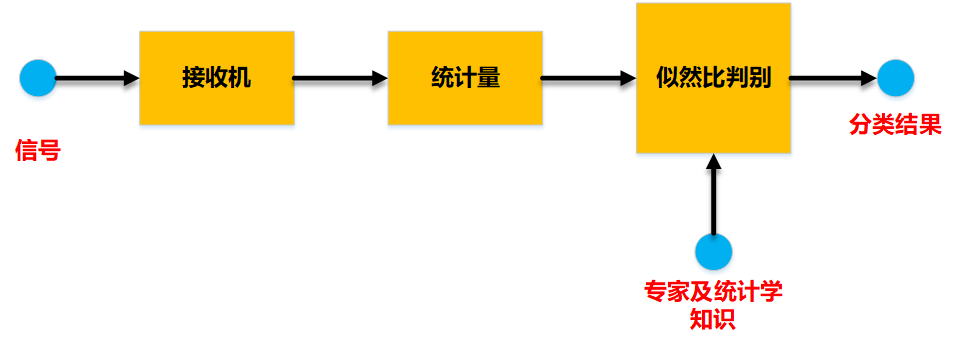
\includegraphics[scale=0.55]{figures/chapter_1/fig_1_0}
	\caption{基于似然比判决理论的调制识别系统框图} \label{sec:fig_1_0}
\end{figure}

对于现有调制识别的发展,Kim和Polydoros\cite{kim1988digital}使用平均似然比检验来识别BPSK和QPSK信号。
Hwang等人通过似然方法法解决了数字正交偏移调制信号的分类问题\cite{hwang1991advanced},
Chung-Yu Huan等人针对加性高斯白噪声中对MPSK调制进行分类的问题,
提出了基于似然函数及其近似的算法\cite{380199}。
Schreyoegg等人提出了一种分类QAM信号的星座图方法,
主要通过分析幅度分布和相位直方图的DFT来对多种QAM信号进行区分\cite{644992}。 
Wei和Mendel将最大似然方法应用于数字正交调制的分类,并分析了最大似然分类器的渐近行为,
当信噪比为5dB时,准确率接近$100%$\cite{wei2000maximum}。
Boiteau等人提出了一种广义的似然比调制识别框架,作者首先对似然比函数中自然指数进行幂级数展开,
然后对未知参数做期望平均处理,实质上应用了高阶统计量\cite{boiteau1998general}。
\par

基于似然比决策理论的算法的优势是:在理论上保证贝叶斯最小误判准则,使分类结果最优;
同时,它可以通过理论分析得到分类性能曲线。
但是他同时具有很多局限性:
首先,现有的似然比决策理论算法主要处理符号的同步采样序列,他们需要比模式识别方法更多的先验知识,
这意味着我们需要预先知道信号的载波频率,符号速率和符号时序等先验信息;
其次,基于未知参数似然比的分类,需要计算复杂的统计表达式,计算成本较高,很难对信号进行实时处理;
第三,基于似然比决策的算法对模型失配和参数偏差较为敏感,即鲁棒性较差。
基于似然比函数的分类,通常将参数值建模为高斯分布,并且需体现知道信噪比等参数。
当实际信道噪声为非高斯噪声时,或者存在多径影响、多信号干扰以及SNR参数估计偏差较大时,
分类的性能可能会急剧下降。\par
 
\subsection{基于特征提取的统计机器学习方法}

基于统计机器学习的调制识别系统大都具有相同的范式:
首先从信号中提取先前选择的特征,然后利用训练好的机器学习模型进行调制识别。
它主要包括特征提取子系统和机器学习子系统,其整体系统框架如图\ref{sec:fig_1_1}所示。\par

\begin{figure}
	\centering
	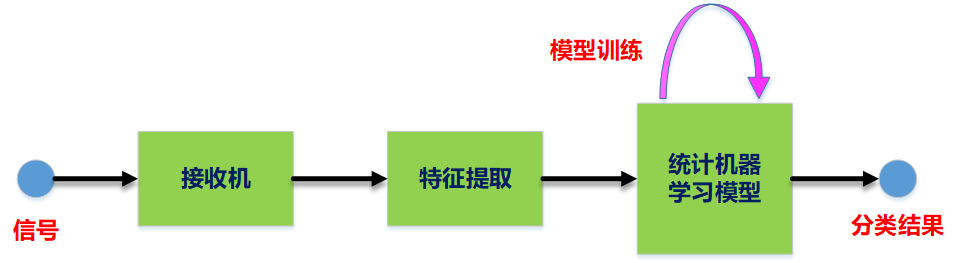
\includegraphics[scale=0.6]{figures/chapter_1/fig_1_1}
	\caption{基于统计机器学习的调制识别系统框图} \label{sec:fig_1_1}
\end{figure}

特征提取子系统主要从未处理信号中提取所需的特征分量,如瞬时频率,瞬时相位和瞬时幅度等。 
模式识别子系统的主要功能是通过特征子系统提取的特征分量对模型进行训练;
模型训练好以后,当需要判别的信号进入该子系统,我们的模型可以对不同的调制信号进行分类。\par

Liedtke提出了一种用于未知调制方法分类的通用分类器,
对数字调制信号识别方法首先进行公开讨论\cite{liedtke1984computer}。 
该算法主要对幅移键控(ASK),具有小频偏的频移键控(FSK)和相移键控(PSK)等信号进行了识别,对于噪声、中心频率、带宽不匹配,以及邻域信号串扰等干扰条件,具有较强的可靠性和鲁棒性。 
Azzouz等人提出了一套用于识别不同类型数字调制方式的判别标准,
它使用相位的非线性部分及其绝对值,归一化的瞬时振幅和频率等特征,
在信噪比SNR = 10dB时,调制类型分类正确率率大于$90\%$\cite{azzouz1995automatic}。
M.L.D. Wong和AK Nandi等人提出了利用多层感知机进行调制识别的算法,
该算法具有更好的泛化能力,并增加了一个新的基于统计累积量的特征集来识别十种不同的调制类型;
即使在低信噪比条件下,该算法也具备较好的性能,
在SNR=0dB时,识别准确率可以达到$98\%$\cite{wong2001automatic}。
文献\cite{汤卫东2010基于小波变换的数字通信信号调制识别研究}中利用小波变化对调制
信号进行了类内和类间识别,提高了低信噪比条件下的识别率。
杨发权在其博士论文中,对高维数据块正交调制识别方法进行应用,并对MLP在调制识别中的应用进行了研究,
实现了在低信噪比条件下基于星座图的调制识别\cite{杨发权2015无线通信信号调制识别关键技术与理论研究}。\par

高阶统计量是描述随机过程的高阶统计特性的数学工具,包括高阶矩和高阶累积量,以及高阶周期矩和循环累积量。
Reichert和Juergen首次提出使用高阶统计量来识别2ASK,2PSK, 4PSK,2FSK,MSK等信号,
之后基于高阶统计量的调制信号识别方法取得了很大进展\cite{reichert1992automatic}。
Swami提出了一种基于四阶累积量的数字调制识别的算法,对2ASK,2PSK,4PSK,MSK和2FSK的信号进行识别,
当信噪比为7.3dB以下时,识别率都能超过$97.9\%$\cite{swami2000hierarchical}。
Gardner和Spooner第一次将循环谱域的结构可分性应用到信号分类,
之后KIM等人利用循环谱特性构建分类器来识别SQPSK和$2^kPSK$信号。\par

基于星座的调制识别将调制识别问题转化为形状识别问题。
Mobasseri首先提出了星座图作为调制识别的一种强特征,
利用二项非均匀空间随机场恢复星座图,并利用机器学习算法作为分类器,
在高噪声环境中具备较强的稳定性\cite{mobasseri1999constellation}。
接下来,Mobasseri又证明模糊c均值聚类能够恢复未知星座,使用星座形状作为数字调制识别的强特征,
通过ML规则对未知星座形状的信号进行分类,
该算法适用于任意大小和维度的数字调制\cite{mobasseri2000digital}。\par
 
对于以上提到的各种分类特征,包括时频统计特征,高阶统计量,星座特征等,
大部分是针对特定类型信号的,而不是对所有的信号都具备一定的辨识能力。
另外,大多数现有的调制识别算法都假定信道是理想的高斯白噪声信道,并且只有少数算法研究了衰落信道。
在实际应用中,无线信道的衰落现象不容忽视,多径效应使得传输信号间存在码间干扰等。
在基于理想高斯白噪声信道环境的识别算法中,信噪比较高时识别性能较好;
当信噪比较低时,算法估计的瞬时包络,相位和频率参数可能会存在较大的误差,使系统的识别性能急剧下降,
并且稳定性差,不能满足实际应用的需求。\par

\subsection{基于深度学习的无线调制识别方法}

深度学习是机器学习中一种基于对数据进行表征学习的方法。
深层神经网络是由一系列层组成网络,其中每一层通常是由已知的具有可调参数和非线性激活函数的线性单元组成,
使得深度网络最后可以拟合高度非线性的函数。\par
深度学习在通信领域的应用,带来了新的机遇与变革。
O'Shea等人第一次将卷积神经网络(Convolutional Neural Network, CNN)引入调制识别,证明了深度学习可以应用在调制识别领域,
并且在低信噪比条件下具有更加稳定的性能\cite{o2016convolutional};
此外,作者还提供了一个用于调制识别学习的基准数据集\cite{o2016radio}。
Mendis等人将深度置信网络(Deep Belief Networks, DBN)引入到调制识别,
在多径信道下,信噪比在$0dB$以上时检测准确率达到$90\%$以上,分类准确率达到$85\%$以上\cite{mendis2016deep}。
Afan等人提出了一种基于非负约束自编码器的自动调制分类的方法\cite{ali2017automatic}。
相较于传统的稀疏编码,该方法提高了稀疏性并使重构误差最小,在有限的信号长度和衰落信道条件下具有较高的准确率。
Rajendran等人提出了一个基于长短期记忆网络(Long Short-Term Memory,LSTM)的调制识别网络,
在信号的信噪比从0dB到20dB的不同SNR条件下,
平均分类准确率为90%左右\cite{rajendran2017distributed}。
Bin Tang提出了一种基于生成对抗网络(Generative Adversarial Net-works,GAN)增强的通信信号调制分类算法,
弥补数据不足对网络训练的影响,作者提出增强数据的方法,
使模型的分类精度可以提高$0.1\% \sim 6.0\%$ \cite{8319926}。\par

以上的研究主要是从应用的层面对深度学习的既有方法进行不同领域的迁移应用,
并没有提出一定的算法框架或者底层网络结构的改进,而且对于影响性能的因素,算法所能达到的上限,
以及将深度学习与传统的调制识别方法结合方面都没有进行相应的研究。
因此,需要我们对深度学习在调制识别中的应用在算法、框架、应用等层面进行更深入的研究,
以提高系统的调制识别性能。\par

\section{本文主要工作及内容安排}
从现有的研究成果可以看出,虽然数字通信信号的调制识别算法有很多,
但能够直接利用原始数据对调制信号进行识别的算法还比较少,大多都需要手动进行专家特征提取,
进而训练机器学习模型进行调制识别。
而在实际的非协作通信中,受环境的影响,我们学习的模型在不同的环境中分类性能差别很大,鲁棒性较差。
现有的基于深度学习的调制识别算法,并没有对影响网络性能的因素进行分析,也没能有效利用过去几十年的研究成果。\par

本文提出了一种基于卷积自编码器和卷积神经网络框架
(Convolutional Autoencoder - Convolutional Neural Network,CAE-CNN)的调制识别算法,
并提出了相应框架下的网络训练方法;
提出了一种将深度特征与传统特征进行融合的算法框架,并对特征融合的方式进行了研究;
研究了网络的深度、网络底层模块结构等对调制识别性能的影响,分析了不同情况下造成网络识别性能变化的因素。 \par

本文的具体内容安排如下:

第一章为绪论。首先对无线信号调制识别技术的研究背景进行了介绍,
系统的阐述了现有的调制识别的算法,并对当前的研究现状进行了总结概括。\par

第二章首先介绍了调制信号的基本概念,然后分析了信道对于调制识别的影响;接下来,介绍
了神经元、前馈神经网络、卷积神经网络、自编码器等深度学习的基本
理论和基本网络架构;最后,介绍了最近较为流行的几种神经网络优化算法,并分析
了各种算法的一些理论基础。 \par

第三章提出了一种CAE-CNN调制识别的算法框架,并提出了相应的训练算法。
我们分别利用监督方法和无监督方法将信号特征可视化,
利用无监督的卷积自编码器可以复现输入信号,并获得原始信号的低维表示;
通过有监督的CNN获取的信号低维表示,得到对于不同类别具有区分度的特征;
利用t-SNE算法,将信号的低维表示降到二维的流型中,观察了信号的分布状况。
我们融合卷积自编码器与卷积神经网络,提出了一种CAE-CNN算法框架和相应训练算法。\par

第四章提出了一种传统特征与深度特征融合的框架。
首先概括了传统调制所用到的调制识别特征,然后阐述了体征融合的基本理论。
接下来,将传统方法中常用的调制识别的特征与CNN获取的深度特征进行适应性的$Batch-Normalization$,
分别针对Softmax、随机森林、深度神经网络等融合算法构建融合模型,
并对不同融合算法的进行了仿真仿真。 \par

第五章从网络底层研究网络超参数对调制识别性能的影响,并从欠拟合
与过拟合以及偏差与方差的角度来理解出现这些现象的原因。
首先,构建了调制识别模型的偏差与方差模型,并阐述了过拟合与欠拟合的原因;
然后,基于CNN网路框架研究了卷积核数目、大小以及卷基层深度对调制识别的影响。\par

第六章对本文的工作进行了总结,从深度框架、特征融合、网络超参数等三个点阐述了
本文所做出的贡献。同时,对深度学习在调制识别领域的应用进行了展望,对以后打算开展的
研究做了一定的概述。
\par

\chapter{无线信号调制识别以及深度学习理论}
\label{chap: mod_rec_deep_learning_theo}
\section{引言}
在动态频谱接入(DSA)中,感知周围的发射终端,以避免无线电干扰并优化频谱分配,是无线认知的重要组成部分。 广播无线电、本地和广域数据、语音信号、雷达用户以及附近其他潜在无线电干扰源等信号具有不同的调制形式和特征,识别和区分这些信号是通信系统最基本的步骤。因此,需要我们队信号调制方式有一定的了解。本章主要讨论信号调制的基本概念以及深度学习的基础知识。
\section{调制识别}


\subsection{调制信息}
在无线电通信中,信号通常由定义好的和理解的基本功能上的许多调制数据位组成由这些基地形成的离散模式。信号的复合基带表示将无线电电压电平时间序列分解为其对载波频率的正弦和余弦函数的投影。通过操纵频率,幅度,相位或其总和,数据比特然后通过离散和可分离的模式调制到这个空间中,对于数字的每个不同的符号周期,或者在模拟调制的情况下连续的位置。对于QPSK的情况,这个相位映射如4所示。然后通常将脉冲整形滤波器(例如根升余弦)应用于频带限制信号,并消除这些不同模式之间的尖锐宽带瞬态,导致相邻符号在发射机处的基极以确定性和可逆性混合。在我们的模拟数据集中,我们使用一个根升余弦脉冲整形滤波器,每个数字信号的带宽为0.35。\par

\subsection{信道对调制信号的影响}
在传播效应的这些苛刻的现实假设下,对专家特征和决策度量的最优性进行分析建模是非平凡的,并且经常会使得简化假设。 在本文中,我们将重点放在包括所有上述效应在内的苛刻的模拟传播环境中的性能的经验性测量,但不要尝试以封闭形式分析追踪其性能。\par

相比之下,信道效应不是确定性的,在通信系统中不是完全可逆的。真实的系统在传输的信号上经历许多影响,这使得恢复和表示具有挑战性。热噪声在接收器处产生相对平坦的高斯白噪声,其形成本底噪声或灵敏度级别和信噪比。由于温度和其他半导体物理因发射器和接收器的不同而引起的振荡器漂移导致符号时序偏移,采样速率偏移,载波频率偏移和相位差。这些效应导致信道之间的时间移位,缩放,线性混合/旋转以及基于未知时变过程的接收信号的旋转。最后,根据在接收机处发射信号的到达模式,实际信道经历随机滤波,具有不同的幅度,相位,多普勒和延迟。这是一种通常被称为多径衰落或频率选择性衰落的现象,其发生在信号可能反射出建筑物,车辆或环境中的任何形式的反射器的任何环境中。通常在接收机中通过估计时变信道响应的瞬时值并将其从接收信号解卷积来消除这种情况。\par

\section{神经网络概述}
\subsection{神经元概述}
以监督学习为例,假设我们有训练样本集$(x(^i),y(^i))$,那么神经网络算法能够提供一种复杂且非线性的假设模型$h_{W,b}(x)$ ,它具有参数$W, b$,可以以此参数来拟合我们的数据。图\ref{fig_2_1}即是“神经元”的图示:\par
\begin{figure}[htbp]
	\centering
	% Requires \usepackage{graphicx}
	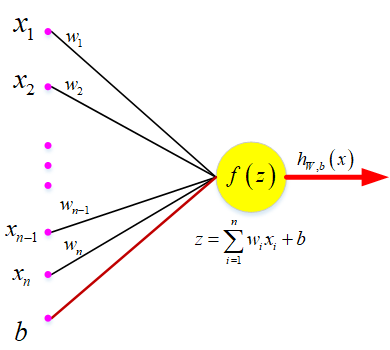
\includegraphics[scale=1]{figures/chapter_2/fig_2_1.png}\\
	\caption{神经元示意图}\label{fig_2_1}
\end{figure}
这个“神经元”是一个以$x_1, x_2, x_3$ 及截距$+1$ 为输入值的运算单元,其输出为:
\begin{equation}
	h_{W,b}(x) = f(W^Tx) = f(\sum_{i=1}^3 w_{i}x_i +b)
\end{equation} 
其中函数$f : \Re \mapsto \Re$被称为“激活函数”。在本论文中,我们一般选用$ReLU$函数作为激活函数$f(\cdot)$:
\begin{equation}
	f(z) = 
	\begin{cases}
		1 & z <=0\\
		z & z > 0
	\end{cases}
\end{equation}
可以看出,$ReLU$激活函数在输入值小于零时输出为0,在大于0时为一条经过原点的直线,其相较于$Sigmoid$激活函数而言,具有如下优点:单侧抑制 ,相对宽阔的兴奋边界 ,稀疏激活性。\par

图\ref{sec:fig_2_2}和图\ref{sec:fig_2_3}分别是$ReLU$及$Sigmoid$的函数图像:

\begin{figure}[htbp]
	\centering
	\begin{minipage}[t]{0.48\textwidth}
		\centering
		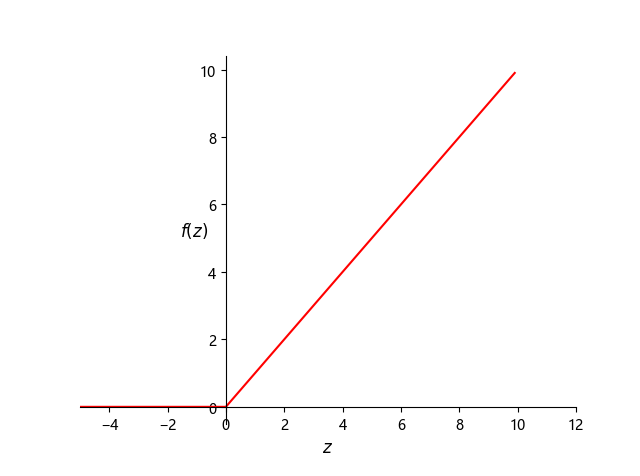
\includegraphics[width=8cm]{figures/chapter_2/fig_2_2.png}
		\caption{$ReLU$函数}\label{sec:fig_2_2}
	\end{minipage}
	\begin{minipage}[t]{0.48\textwidth}
		\centering
		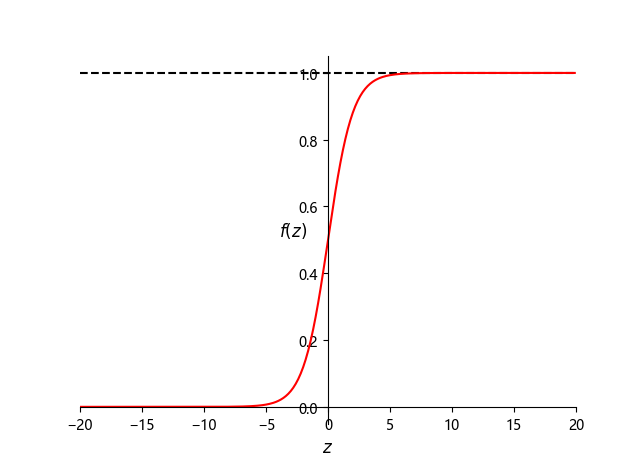
\includegraphics[width=8cm]{figures/chapter_2/fig_2_3.png}
	\end{minipage}
	\caption{$Sigmoid$函数}\label{sec:fig_2_3}
\end{figure}

%\begin{figure}[!h]
%	\centering
%	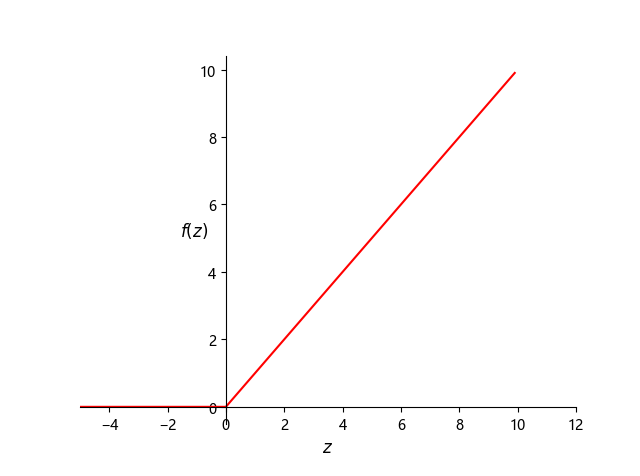
\includegraphics[scale=0.5]{figures/chapter_2/fig_2_2.png}
%	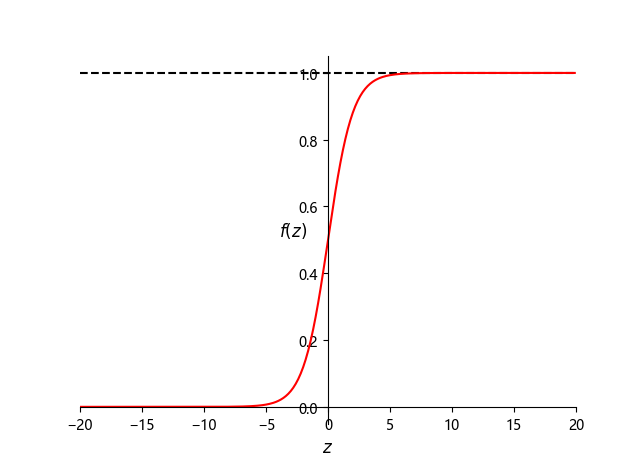
\includegraphics[scale=0.5]{figures/chapter_2/fig_2_3.png}
%	\caption{$ReLU$函数与$Sigmoid$函数}\label{sec:fig_2_2}
%\end{figure}

\subsection{前馈神经网络}
前馈神经网络就是将许多个单一“神经元”联结在一起,这样,一个“神经元”的输出就可以是另一个“神经元”的输入。例如,图\ref{sec:fig_2_4}就是一个简单的神经网络:\par
\begin{figure}
	\centering
	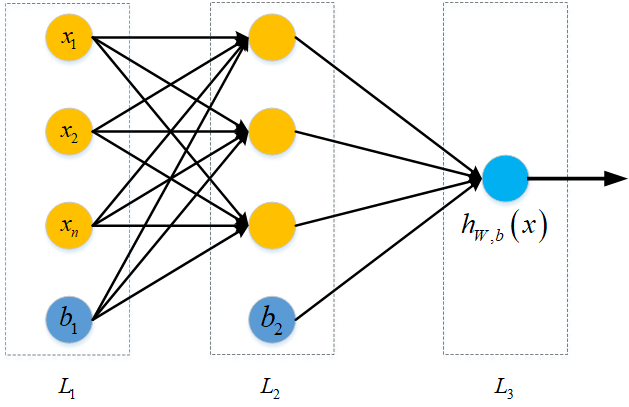
\includegraphics[scale=0.7]{figures/chapter_2/fig_2_4}\label{sec:fig_2_4}
	\caption{前馈神经网络}\label{fig_2_4}
\end{figure}
我们使用圆圈来表示神经网络的输入,标上“$+1$”的圆圈被称为偏置节点,也就是截距项。神经网络最左边的一层叫做输入层,最右的一层叫做输出层(本例中,输出层只有一个节点)。中间所有节点组成的一层叫做隐藏层,因为我们不能在训练样本集中观测到它们的值。同时可以看到,以上神经网络的例子中有3个输入单元(偏置单元不计在内),3个隐藏单元及一个输出单元。\par

 我们用 来表示网络的层数,本例中 ,我们将第 层记为 ,于是 是输入层,输出层是 。] 我们用$a^{(l)}_i$表示第$l$层第$i$单元的激活值(输出值)。当$l=1$时,$a^{(1)}_i = x_i$,也就是第$i$个输入值(输入值的第$i$个特征)。对于给定参数集合$W,b$,我们的神经网络就可以按照函数$h_{W,b}(x)$来计算输出结果。\par
 
我们用$z^{(l)}_i$表示第$l$层第$i$单元输入加权和(包括偏置单元)

我们将上面的计算步骤叫作前向传播。回想一下,之前我们用$a^{(1)} = x$表示输入层的激活值,那么给定第$l$层的激活值$a^{(l)}$后,第$l+1$层的激活值$a^{(l+1)}$就可以按照下面步骤计算得到:
\begin{align}
	z^{(l+1)} &= W^{(l)} a^{(l)} + b^{(l)}=\sum_{j=l}^n W^{(l)}_{ij} x_j + b^{(l)}_i\\
	a^{(l+1)} &= f(z^{(l+1)})
\end{align}
将参数矩阵化,使用矩阵-向量运算方式,我们就可以利用线性代数的优势对神经网络进行快速求解。\par

目前为止,我们讨论了一种神经网络,我们也可以构建另一种结构的神经网络(这里结构指的是神经元之间的联接模式),也就是包含多个隐藏层的神经网络。最常见的一个例子是$n_l$层的神经网络,第$1$ 层是输入层,第$n_l$层是输出层,中间的每个层$l$与层$l+1$紧密相联。这种模式下,要计算神经网络的输出结果,我们可以按照之前描述的等式,按部就班,进行前向传播,逐一计算第$L_2$层的所有激活值,然后是第$L_3$层的激活值,以此类推,直到第$L_{n_l}$ 层。这是一个前馈神经网络的例子,因为这种联接图没有闭环或回路。\par

\subsection{反向传播算法}
假设我们有一个固定样本集$\{ (x^{(1)}, y^{(1)})$, $\ldots$, $(x^{(m)}$, $y^{(m)}) \}$,它包含$m$个样例。我们可以用批量梯度下降法来求解神经网络。具体来讲,对于单个样例$(x,y)$,我们假设其代价函数$J(W,b; x,y)$为方差代价函数,则有:
\begin{align}
	J(W,b; x,y) = \frac{1}{2} \left\| h_{W,b}(x) - y \right\|^2.
\end{align}
给定一个包含$m$个样例的数据集,那么整体代价函数$J(W,b)$为:
\begin{equation}
	\begin{aligned}
	J(W,b)
	&= \left[ \frac{1}{m} \sum_{i=1}^m J(W,b;x^{(i)},y^{(i)}) \right]
	+ \frac{\lambda}{2} \sum_{l=1}^{n_l-1} \; \sum_{i=1}^{s_l} \; \sum_{j=1}^{s_{l+1}} \left( W^{(l)}_{ji} \right)^2
	\\
	&= \left[ \frac{1}{m} \sum_{i=1}^m \left( \frac{1}{2} \left\| h_{W,b}(x^{(i)}) - y^{(i)} \right\|^2 \right) \right]
	+ \frac{\lambda}{2} \sum_{l=1}^{n_l-1} \; \sum_{i=1}^{s_l} \; \sum_{j=1}^{s_{l+1}} \left( W^{(l)}_{ji} \right)^2
	\end{aligned}
\end{equation}
以上关于$J(W,b)$定义中的第一项是一个均方差项。第二项是一个规则化项(也叫权重衰减项),其目的是减小权重的幅度,防止过度拟合。
权重衰减参数$\lambda$用于控制公式中两项的相对重要性。

以上的代价函数经常被用于分类和回归问题。在分类问题中,我们用$y=0$或$1$,来代表两种类型的标签(回想一下,这是因为sigmoid激活函数的值域为$[0,1]$;如果我们使用双曲正切型激活函数,那么应该选用$-1$和$+1$ 作为标签)。对于回归问题,我们首先要变换输出值域,以保证其范围为$[0,1]$(同样地,如果我们使用双曲正切型激活函数,要使输出值域为$[-1,1]$)。\par

反向传播算法的思路如下:给定一个样例$(x,y)$,我们首先进行“前向传导”运算,计算出网络中所有的激活值,包括$h_{W,b}(x)$的输出值。之后,针对第$l$层的每一个节点$i$,我们计算出其“残差”$\delta^{(l)}_i$,该残差表明了该节点对最终输出值的残差产生了多少影响。对于最终的输出节点,我们可以直接算出网络产生的激活值与实际值之间的差距,我们将这个差距定义为$\delta^{(n_l)}_i$(第$n_l$层表示输出层)。对于隐藏单元我们如何处理呢?我们将基于节点残差的加权平均值计算$\delta^{(l)}_i$,这些节点以$a^{(l)}_i$作为输入。反向传播算法可表示为以下几个步骤:\par
进行前馈传导计算,利用前向传导公式,得到$L_2, L_3$, $\ldots$直到输出层$L_{n_l}$的激活值。
对输出层(第$n_l$层),计算:
\begin{align}
	\delta^{(n_l)}
	= - (y - a^{(n_l)}) \bullet f'(z^{(n_l)})
\end{align}
对于$l = n_l-1, n_l-2, n_l-3$, $\ldots$, $2$的各层,计算:
\begin{align}
	\delta^{(l)} = \left((W^{(l)})^T \delta^{(l+1)}\right) \bullet f'(z^{(l)})
\end{align}
计算最终需要的偏导数值:
\begin{align}
	\nabla_{W^{(l)}} J(W,b;x,y) &= \delta^{(l+1)} (a^{(l)})^T, \\
	\nabla_{b^{(l)}} J(W,b;x,y) &= \delta^{(l+1)}.
\end{align}
实现中应注意:在以上的第2步和第3步中,我们需要为每一个$i$值计算其$f'(z^{(l)}_i)$。假设$f(z)$是sigmoid函数,并且我们已经在前向传导运算中得到了$a^{(l)}_i$。
最后,我们将对梯度下降算法做个全面总结。在下面的伪代码中,$\Delta W^{(l)}$是一个与矩阵$W^{(l)}$维度相同的矩阵,$\Delta b^{(l)}$是一个与$b^{(l)}$维度相同的向量。注意这里“$\Delta W^{(l)}$”是一个矩阵,而不是“$ \Delta$与$W^{(l)}$相乘”。下面,我们实现批量梯度下降法中的一次迭代:\par

对于所有$l$,令$\Delta W^{(l)} := 0$, $\Delta b^{(l)} := 0 $(设置为全零矩阵或全零向量)
对于$i = 1$到$m$,
使用反向传播算法计算$\nabla_{W^{(l)}} J(W,b;x,y)$和$\nabla_{b^{(l)}} J(W,b;x,y)$。
计算$\Delta W^{(l)} := \Delta W^{(l)} + \nabla_{W^{(l)}} J(W,b;x,y)$。
计算$\Delta b^{(l)} := \Delta b^{(l)} + \nabla_{b^{(l)}} J(W,b;x,y)$。
更新权重参数:
\begin{align}
	W^{(l)} &= W^{(l)} - \alpha \left[ \left(\frac{1}{m} \Delta W^{(l)} \right) + \lambda W^{(l)}\right] \\
	b^{(l)} &= b^{(l)} - \alpha \left[\frac{1}{m} \Delta b^{(l)}\right]
\end{align}
现在,我们可以重复梯度下降法的迭代步骤来减小代价函数$J(W,b)$的值,进而求解我们的神经网络。

\section{卷积神经网络}
卷积网络,也叫做卷积神经网络,是一种专门用来处理具有类似网格结构的数据的神经网络。
例如时间序列数据(可以认为是在时间轴上有规律地采样形成的一维网格)和图像数据(可以看作是二维的像素网格)。
卷积网络在诸多应用领域都表现优异。卷积是一种特殊的线性运算。
\emph{卷积网络是指那些至少在网络的一层中使用卷积运算来替代一般的矩阵乘法运算的神经网络。}\par

\subsection{卷积运算}
\label{sec:the_convolution_operation}

卷积是对两个实变函数的一种数学运算,通常我们用星号表示:
\begin{equation}
s(t) = (x*w)(t) = \int x(\tau)w(t-\tau)d\tau
\end{equation}

在卷积网络的术语中,卷积的第一个参数(在这个例子中,函数$x$)通常叫做输入,第二个参数(函数$w$)叫核函数。
输出有时被称作特征映射。

如果我们假设$x$和$w$都定义在整数时刻$t$上,则卷积的离散形式:
\begin{equation}
s(t) = (x*w)(t) = \sum_{\tau = -\infty}^{\infty} x(\tau)w(t\tau).
\end{equation}

在机器学习的应用中,输入通常是多维数组的数据,而核通常是由学习算法优化得到的多维数组的参数。
我们把这些多维数组叫做张量。
因为在输入与核中的每一个元素都必须明确地分开存储,我们通常假设在存储了数值的有限点集以外,这些函数的值都为零。
这意味着在实际操作中,我们可以通过对有限个数组元素的求和来实现无限求和。

在处理图像数据时,我们经常一次在多个维度上进行卷积运算。如果把一张二维的图像$I$作为输入,同时使用使用一个二维的核$K$,则有:
\begin{equation}
S(i,j) = (I*K)(i,j) = \sum_m \sum_n I(m,n) K(i-m, j-n).
\end{equation}

卷积是可交换的(commutative),我们可以等价地写作:
\begin{equation}
S(i, j) = (K*I)(i,j) = \sum_m \sum_n I(i-m, j-n) K(m, n).
\end{equation}

卷积运算可交换性的出现是因为我们将核相对输入进行了翻转,从$m$增大的角度来看,输入的索引在增大,但是核的索引在减小。
我们将核翻转的唯一目的是实现可交换性。
许多神经网络库会实现一个相关的函数,称为互相关函数,和卷积运算几乎一样但是并没有对核进行翻转:
\begin{equation}
S(i, j) = (I*K)(i, j) = \sum_m \sum_n I(i+m, j+n) K(m, n).
\end{equation}
许多机器学习的库实现的是互相关函数但是称之为卷积,在本文中,我们将这两种运算都称之为卷积运算。\par

\subsection{卷积特性}
卷积运算通过三个重要的思想来帮助改进机器学习系统:稀疏交互、参数共享、等变表示。

传统的神经网络使用矩阵乘法来建立输入与输出的连接关系。
对于卷积,参数共享的特殊形式使得神经网络层具有对平移等变的性质。
如果一个函数满足输入改变,输出也以同样的方式改变这一性质,我们就说它是等变(equivariant)的。
特别地,如果函数$f(x)$与$g(x)$满足$f(g(x))= g(f(x))$,我们就说$f(x)$对于变换$g$具有等变性。
对于卷积来说,如果令$g$是输入的任意平移函数,那么卷积函数对于$g$具有等变性。
当处理时间序列数据时,这意味着通过卷积可以得到一个由输入中出现不同特征的时刻所组成的时间轴。
如果我们把输入中的一个事件向后延时,在输出中仍然会有完全相同的表示,只是时间延后了。
而这也正好对应到我们无线信号中的时移不变性。因此,我们可以很好的将\label{con_net}应用到调制信号识别中。\par

\subsection{卷积作为一种无限强的先验}
先验被认为是强或者弱取决于先验中概率密度的集中程度。
弱先验具有较高的熵值,例如方差很大的高斯分布。这样的先验允许数据对于参数的改变具有或多或少的自由性。
强先验具有较低的熵值,例如方差很小的高斯分布。这样的先验在决定参数最终取值时起着更加积极的作用。
一个无限强的先验需要对一些参数的概率置零并且完全禁止对这些参数赋值,无论数据对于这些参数的值给出了多大的支持。\par

我们可以把卷积网络类比成全连接网络,但对于这个全连接网络的权重有一个无限强的先验。
这个无限强的先验是说一个隐藏单元的权重必须和它邻居的权重相同,但可以在空间上移动。
这个先验也要求除了那些处在隐藏单元的小的空间连续的接受域内的权重以外,其余的权重都为零。

总之,我们可以把卷积的使用当作是对网络中一层的参数引入了一个无限强的先验概率分布。
这个先验说明了该层应该学得的函数只包含局部连接关系并且对平移具有等变性。

\subsection{随机或无监督的特征}
\label{sec:random_or_unsupervised_features}

通常,卷积网络训练中最耗时的部分是学习特征。 
输出层的计算代价通常相对不高,因为在通过若干层卷积池化之后作为该层输入的特征的数量较少。
当使用梯度下降执行监督训练时,每步梯度计算需要完整地运行整个网络的前向传播和反向传播。
减少卷积网络训练成本的一种方式是使用那些不是由监督方式训练得到的特征。\par

有三种基本策略可以不通过监督训练而得到卷积核。
其中一种是简单地随机初始化它们。
另一种是手动设计它们,例如设置每个核在一个特定的方向或尺度来检测边缘。
最后,可以使用无监督的标准来学习核。\par

使用无监督的标准来学习特征,允许这些特征的确定与位于网络结构顶层的分类层相分离。
然后只需提取一次全部训练集的特征,构造用于最后一层的新训练集。
假设最后一层类似逻辑回归或者支持向量机,那么学习最后一层通常是凸优化问题。\par


随机过滤器经常在卷积网络中表现得出乎意料得好~\cite{Jarrett-ICCV2009-small,Saxe-ICML2011,pinto2011scaling,cox2011beyond}。
\cite{Saxe-ICML2011}~说明,由卷积和随后的池化组成的层,当赋予随机权重时,自然地变得具有频率选择性和平移不变性。
他们认为这提供了一种廉价的方法来选择卷积网络的结构:首先通过仅训练最后一层来评估几个卷积网络结构的性能,然后选择最好的结构并使用更昂贵的方法来训练整个网络。
一个中间方法是学习特征,但是使用那种不需要在每个梯度计算步骤中都进行
完整的前向和反向传播的方法。与多层感知机一样,我们使用贪心逐层预训练,单
独训练第一层,然后一次性地从第一层提取所有特征,之后用那些特征单独训练
第二层,以此类推。



\section{卷积自编码器}

自动编码器是一种无监督的学习算法,其中神经网络的优化目标是通过一些更有约束的中间维度,使用均方误差(MSE)等损失函数,最小化输出处的重构误差。
自编码器可以理解为一个试图去还原其原始输入的系统。它通过约束网络的中间层维度,从而可以通过提取用于聚类的中间稀疏编码,来获得原始数据的非线性降维。在这种情况下,使用相似的调制信号,可以由相似的卷积核和特征图来表示,因此,他们分布在该压缩空间的相近区域中。自编码器中的卷积层具有时移不变性以及受约束的参数搜索空间(相对于全连接层),因此非常适合于无线电时间序列信号表示。我们使用dropout[13]并在输入层加入噪声[7]对网络进行正则化,来增强模型的泛化能力。如下图所示。
\begin{figure}[!h]
	\centering
	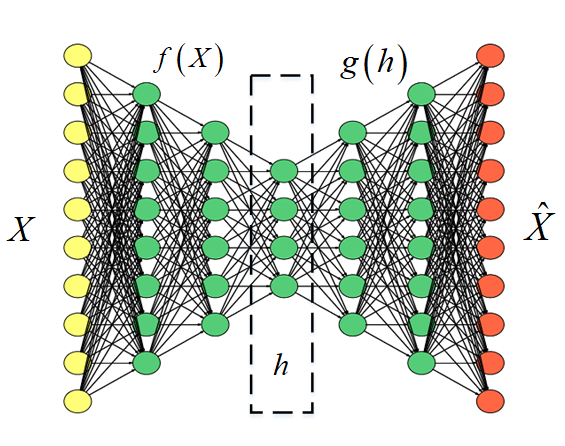
\includegraphics[scale=0.7]{figures/chapter_2/fig_2_5}
	\caption{自编码器}	\label{fig_2_5}
\end{figure}

图中,虚线蓝色框内就是一个自编码器模型,它由编码器(Encoder)和解码器(Decoder)两部分组成,本质上都是对输入信号做某种变换。编码器将输入信号x变换成编码信号y,而解码器将编码信号y转换成输出信号。即:
\begin{equation}
	\begin{gathered}
		h=f(X)
		\\
		\hat{X}=g(h)=g(f(X))
	\end{gathered}
\end{equation}
而自编码器的目的是,让输出尽可能复现输入x。对于自编码器,我们往往并不关心输出是什么(反正只是复现输入),我们真正关心的是中间层的编码信号,或者说是从输入到编码的映射。在我们强迫编码信号y和输入信号x不同的情况下,系统还能够去复原原始信号x,那么说明编码信号y已经承载了原始数据的所有信息,但以一种不同的形式,这便是特征提取。对于卷积自便器,我们中间的隐层是利用卷积网络实现的。\par

通常,自编码器利用反向传播算法,将误差进行反向传播,并使用随机梯度下降(SGD)算法等,以找到接近等式\ref{sec:eqt2_3}中的最佳网络参数。

\begin{equation}\label{sec:eqt2_3}
\mathop{\arg\min}_{\theta} \sum(X − \hat{X})^2
\end{equation}

在自编码器的训练过程中,我们尽量减少重构均方误差(MSE),但由于我们的主要目标是获得一个良好的聚类稀疏表示,我们显着限制隐藏层维度到一个点,我们的重构作出一些可见的简化假设,在最优重构误差下降低了隐层维数。图3显示了两个训练样例,2x128输入向量的样子,1x30稀疏表示的样子,以及2x128输出重构的样子。这给了这个网络的学习代表能力的一些直觉。\par


\section{\glssymbol{LSTM}}
\label{sec:lstm}
\label{chap:sequence_modeling_recurrent_and_recursive_nets}
\gls{RNN}或~\glssymbol{RNN}是一类用于处理序列数据的\gls{NN}。
就像\gls{convolutional_network}是专门用于处理网格化数据的\gls{NN},\gls{RNN}是专门用于处理序列$x^{(1)}, \dots, x^{(\tau)}$的\gls{NN}。

正如\gls{convolutional_network}可以很容易地扩展到具有很大宽度和高度的图像,以及处理大小可变的图像,\gls{recurrent_network}可以扩展到更长的序列(比不基于序列的特化网络长得多)。
大多数\gls{recurrent_network}也能处理可变长度的序列。

\begin{figure}[!h]
	\centering
	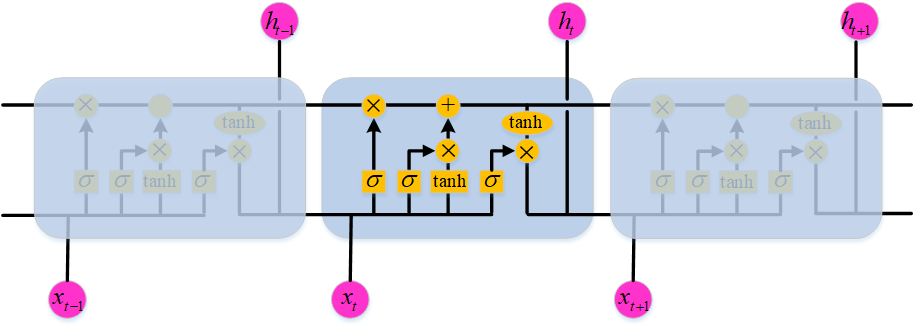
\includegraphics[scale=0.7]{figures/chapter_2/fig_2_6.png}
	\caption{\glssymbol{LSTM}~\gls{recurrent_network}``细胞''的框图。
		细胞彼此循环连接,代替一般\gls{recurrent_network}中普通的\gls{hidden_unit}。
		这里使用常规的人工神经元计算输入特征。
		如果sigmoid输入门允许,它的值可以累加到状态。
		状态单元具有线性自循环,其权重由\gls{forget_gate}控制。
		细胞的输出可以被输出门关闭。
		所有\gls{gated}单元都具有sigmoid非线性,而输入单元可具有任意的压缩非线性。
		状态单元也可以用作\gls{gated}单元的额外输入。
		黑色方块表示单个\gls{time_step}的延迟。
	}\label{fig:chapter2_lstm_cell}
\end{figure}

\glssymbol{LSTM}~块如\figref{fig:chapter2_lstm_cell}所示。
在浅\gls{recurrent_network}的架构下,相应的\gls{forward_propagation}公式如下。
更深的架构也被成功应用\citep{Graves-et-al-ICASSP2013,Pascanu-et-al-ICLR2014}。
\glssymbol{LSTM}~\gls{recurrent_network}除了外部的~\glssymbol{RNN}~循环外,还具有内部的``\glssymbol{LSTM}~细胞''循环(自环),因此~\glssymbol{LSTM}~不是简单地向输入和循环单元的仿射变换之后施加一个逐元素的非线性。
与普通的\gls{recurrent_network}类似,每个单元有相同的输入和输出,但也有更多的参数和控制信息流动的\gls{gated}单元系统。

最重要的组成部分是状态单元$s_i^{(t)}$,与前一节讨论的\gls{leaky_unit}有类似的线性自环。
然而,此处自环的权重(或相关联的时间常数)由\firstgls{forget_gate}~$f_i^{(t)}$控制(时刻$t$和细胞$i$),由~\ENNAME{sigmoid}~单元将权重设置为0和1之间的值:

\begin{equation}
f_i^{(t)} = \sigma \Big( b_i^f + \sum_j U_{i,j}^f x_j^{(t)} + \sum_j W_{i,j}^f h_j^{(t-1)} \Big),
\end{equation}

其中$x^{(t)}$是当前输入向量,$h^{t}$是当前隐藏层向量,$h^{t}$包含所有~\glssymbol{LSTM}~细胞的输出。 
$b^f, U^f, W^f$分别是\gls{bias_aff}、输入权重和\gls{forget_gate}的循环权重。
因此~\glssymbol{LSTM}~细胞内部状态以如下方式更新,其中有一个条件的自环权重$f_i^{(t)}$:

\begin{align}
s_i^{(t)} = f_i^{(t)}  s_i^{(t-1)} +  g_i^{(t)}
\sigma \Big( b_i + \sum_j U_{i,j} x_j^{(t)} + \sum_j W_{i,j} h_j^{(t-1)} \Big),
\end{align}

其中$b, U, W$分别是~\glssymbol{LSTM}~细胞中的\gls{bias_aff}、输入权重和\gls{forget_gate}的循环权重。
\textbf{外部输入门}(external input gate)单元$g_i^{(t)}$以类似\gls{forget_gate}(使用\ENNAME{sigmoid}获得一个0和1之间的值)的方式更新,但有自身的参数:

\begin{align}
g_i^{(t)} = \sigma \Big( b_i^g + \sum_j U_{i,j}^g x_j^{(t)} + \sum_j W_{i,j}^g h_j^{(t-1)} \Big).
\end{align}

\glssymbol{LSTM}~细胞的输出$h_i^{(t)}$也可以由\textbf{输出门}(output gate)~$q_i^{(t)}$关闭(使用\ENNAME{sigmoid}单元作为\gls{gated}):

\begin{align}
h_i^{(t)} &= \text{tanh}\big( s_i^{(t)} \big) q_i^{(t)}, \\
q_i^{(t)} &= \sigma \Big( b_i^o + \sum_j U_{i,j}^o x_j^{(t)} + \sum_j W_{i,j}^o h_j^{(t-1)} \Big),
\end{align}

其中$b^o, U^o, W^o$分别是\gls{bias_aff}、输入权重和\gls{forget_gate}的循环权重。
在这些变体中,可以选择使用细胞状态$s_i^{(t)}$作为额外的输入(及其权重),输入到第$i$个单元的三个门,如\figref{fig:chapter2_lstm_cell}所示。
这将需要三个额外的参数。

\glssymbol{LSTM}~网络比简单的循环架构更易于学习\gls{long_term_dependency},先是用于测试\gls{long_term_dependency}学习能力的人工数据集\citep{Bengio-trnn94,Hochreiter+Schmidhuber-1997,chapter-gradient-flow-2001},然后是在具有挑战性的序列处理任务上获得最先进的表现\citep{Graves-book2012,Graves-arxiv2013,Sutskever-et-al-NIPS2014}。

\section{神经网络优化算法}
用于深度模型训练的优化算法与传统的优化算法在几个方面有所不同。 机器学习通常是间接作用的。
在大多数机器学习问题中,我们关注某些性能度量 P,其定义于测试集上并且可能是不可解的。
因此,我们只是间接地优化 P。我们希望通过降低代价函数$J(θ)$来提高 P。
这一点与纯优化不同,纯优化最小化目标 J 本身。训练深度模型的优化算法通常也会包括一些针对机器学习目标函数的特定结构进行的特化。

\subsection{\glsentrytext{SGD}优化算法}
\label{sec:stochastic_gradient_descent_chap8}
\gls{SGD}及其变种很可能是一般\gls{ML}中应用最多的优化算法,特别是在\gls{DL}中。
按照\gls{DGD}抽取$m$个\gls{minibatch}(独立同分布的)样本,通过计算它们梯度均值,
我们可以得到梯度的\gls{unbiased}估计。
展示了如何沿着这个梯度的估计下降。

\begin{algorithm}[ht]
	\caption{\gls{SGD}(\glssymbol{SGD})在第$k$个训练迭代的更新}
	\label{alg:sgd}
	\begin{algorithmic}
		\REQUIRE \gls{learning_rate} $\epsilon_k$
		\REQUIRE 初始参数$\theta$
		\WHILE{停止\gls{criterion}未满足}
		\STATE 从\gls{training_set}中采包含$m$个样本$\{ x^{(1)},\dots, x^{(m)}\}$ 的\gls{minibatch},其中$x^{(i)}$对应目标为$y^{(i)}$
		\STATE 计算梯度估计: $\hat{g} \leftarrow + 
		\frac{1}{m} \nabla_{\theta} \sum_i L(f(x^{(i)};\theta),y^{(i)})$
		\STATE 应用更新:$\theta \leftarrow theta - \epsilon \hat{g}$
		\ENDWHILE
	\end{algorithmic}
\end{algorithm}

\glssymbol{SGD}\,算法中的一个关键参数是\gls{learning_rate}。
之前,我们介绍的\,\glssymbol{SGD}\,使用固定的\gls{learning_rate}。
在实践中,有必要随着时间的推移逐渐降低\gls{learning_rate},
因此我们将第$k$步迭代的\gls{learning_rate}记作$\epsilon_k$。

这是因为\,\glssymbol{SGD}\,中梯度估计引入的噪声源($m$个训练样本的随机采样)并不会在\gls{minimum}处消失。
相比之下,当我们使用\gls{batch}\gls{GD}到达\gls{minimum}时,整个\gls{cost_function}的真实梯度会变得很小,
之后为$\mathbf{0}$,因此\gls{batch}\gls{GD}可以使用固定的\gls{learning_rate}。
保证\,\glssymbol{SGD}\,收敛的一个充分条件是
\begin{equation}
\label{eq:8.12}
\sum_{k=1}^\infty \epsilon_k = \infty,
\end{equation}
且
\begin{equation}
\label{eq:8.13}
\sum_{k=1}^\infty \epsilon_k^2 < \infty.
\end{equation}

实践中,一般会线性衰减\gls{learning_rate}直到第$\tau$次迭代:
\begin{equation}
\label{eq:8.14}
\epsilon_k = (1-\alpha) \epsilon_0 + \alpha \epsilon_\tau
\end{equation}
其中$\alpha = \frac{k}{\tau}$。
在$\tau$步迭代之后,一般使$\epsilon$保持常数。

\subsection{RMSProp优化算法}
\label{sec:rmsprop}
\textbf{RMSProp}算法\citep{Hinton-ipam2012}修改AdaGrad以在\gls{nonconvex}设定下效果更好,
改变梯度积累为指数加权的移动平均。
\gls{adagrad}\,旨在应用于凸问题时快速收敛。
当应用于\gls{nonconvex}函数训练\gls{NN}时,学习轨迹可能穿过了很多不同的结构,最终到达一个局部是凸碗的区域。
AdaGrad根据平方梯度的整个历史收缩\gls{learning_rate},可能使得\gls{learning_rate}在达到这样的凸结构前就变得太小了。
RMSProp使用指数衰减平均以丢弃遥远过去的历史,使其能够在找到凸碗状结构后快速收敛,
它就像一个初始化于该碗状结构的AdaGrad算法实例。

RMSProp的标准形式如\algref{alg:rms_prop}所示,结合Nesterov动量的形式如\algref{alg:rms_nesterov}所示。
相比于AdaGrad,使用移动平均引入了一个新的\gls{hyperparameter}$\rho$,用来控制移动平均的长度范围。

经验上,RMSProp已被证明是一种有效且实用的\gls{DNN}优化算法。
目前它是\gls{DL}从业者经常采用的优化方法之一。


\begin{algorithm}[ht]
	\caption{RMSProp算法}
	\label{alg:rms_prop}
	\begin{algorithmic}
		\REQUIRE 全局\gls{learning_rate} $\epsilon$,衰减速率$\rho$
		\REQUIRE  初始参数$\theta$
		\REQUIRE 小常数$\delta$,通常设为$10^{-6}$(用于被小数除时的数值稳定)
		\STATE 初始化累积变量 $r = 0$
		\WHILE{没有达到停止\gls{criterion}}
		\STATE 从\gls{training_set}中采包含$m$个样本$\{ x^{(1)},\dots, x^{(m)}\}$ 的\gls{minibatch},对应目标为$y^{(i)}$。
		\STATE 计算梯度:$g \leftarrow  
		\frac{1}{m} \nabla_{\theta} \sum_i L(f(x^{(i)};\theta),y^{(i)})$ 
		\STATE 累积平方梯度:$r \leftarrow \rho
		r + (1-\rho) g \odot g$
		\STATE 计算参数更新:$\Delta \theta =
		-\frac{\epsilon}{\sqrt{\delta + r}} \odot g$  \ \  ($\frac{1}{\sqrt{\delta + r}}$ 逐元素应用)
		\STATE 应用更新:$\theta \leftarrow \theta + \Delta \theta$
		\ENDWHILE
	\end{algorithmic}
\end{algorithm}

\subsection{Adam}
\label{sec:adam}
\textbf{Adam}~\citep{kingma2014adam}是另一种\gls{learning_rate}自适应的优化算法,如\algref{alg:adam}所示。
``Adam''这个名字派生自短语``adaptive moments''。
早期算法背景下,它也许最好被看作结合RMSProp和具有一些重要区别的\gls{momentum}的变种。
首先,在Adam中,\gls{momentum}直接并入了梯度一阶矩(指数加权)的估计。
将\gls{momentum}加入RMSProp最直观的方法是将\gls{momentum}应用于缩放后的梯度。
结合缩放的\gls{momentum}使用没有明确的理论动机。
其次,Adam包括偏置修正,修正从原点初始化的一阶矩(\gls{momentum}项)和(非中心的)二阶矩的估计(\algref{alg:adam})。
RMSProp也采用了(非中心的)二阶矩估计,然而缺失了修正因子。
因此,不像Adam,RMSProp二阶矩估计可能在训练初期有很高的偏置。
Adam通常被认为对\gls{hyperparameter}的选择相当鲁棒,尽管\gls{learning_rate}有时需要从建议的默认修改。

\begin{algorithm}[ht]
	\caption{Adam算法}
	\label{alg:adam}
	\begin{algorithmic}
		\REQUIRE 步长 $\epsilon$ (建议默认为: $0.001$)
		\REQUIRE 矩估计的指数衰减速率, $\rho_1$ 和 $\rho_2$ 在区间 $[0, 1)$内。
		(建议默认为:分别为$0.9$ 和 $0.999$)
		\REQUIRE 用于数值稳定的小常数 $\delta$  (建议默认为: $10^{-8}$)
		\REQUIRE 初始参数 $\theta$
		\STATE 初始化一阶和二阶矩变量 $s = 0 $, $r = 0$
		\STATE 初始化\gls{time_step} $t=0$ 
		\WHILE{没有达到停止\gls{criterion}}
		\STATE 从\gls{training_set}中采包含$m$个样本$\{ x^{(1)},\dots, x^{(m)}\}$ 的\gls{minibatch},对应目标为$y^{(i)}$。
		\STATE 计算梯度:$g \leftarrow \frac{1}{m} \nabla_{\theta} \sum_i L(f(x^{(i)};\theta),y^{(i)})$ 
		\STATE $t \leftarrow t + 1$
		\STATE 更新有偏一阶矩估计: $s \leftarrow \rho_1 s + (1-\rho_1) g$
		\STATE 更新有偏二阶矩估计:$r \leftarrow \rho_2 r + (1-\rho_2)  g \odot g$
		\STATE 修正一阶矩的\gls{bias_sta}:$\hat{s} \leftarrow \frac{s}{1-\rho_1^t}$
		\STATE 修正二阶矩的\gls{bias_sta}:$\hat{r} \leftarrow \frac{r}{1-\rho_2^t}$
		\STATE 计算更新:$\Delta \theta = - \epsilon \frac{\hat{s}}{\sqrt{\hat{r}} + \delta}$ \ \  (逐元素应用操作)
		\STATE 应用更新:$\theta \leftarrow \theta + \Delta \theta$
		\ENDWHILE
	\end{algorithmic}
\end{algorithm}

\subsection{选择正确的优化算法}
\label{sec:choosing_the_right_optimization_algorithms}
在本节中,我们讨论了一系列算法,通过自适应每个模型参数的\gls{learning_rate}以解决优化\gls{deep_model}中的难题。
此时,一个自然的问题是:该选择哪种算法呢?

遗憾的是,目前在这一点上没有达成共识。
\cite{Schaul2014_unittests}展示了许多优化算法在大量学习任务上极具价值的比较。
虽然结果表明,具有自适应\gls{learning_rate}(以RMSProp和AdaDelta为代表)的算法族表现得相当鲁棒,不分伯仲,但没有哪个算法能脱颖而出。

目前,最流行并且使用很高的优化算法包括SGD、具\gls{momentum}的SGD、RMSProp、具\gls{momentum}的RMSProp、AdaDelta和Adam。
此时,选择哪一个算法似乎主要取决于使用者对算法的熟悉程度(以便调节\gls{hyperparameter})。

\section{本章小结}
\chapter{基于CAE-CNN的无线信号调制识别}

\section{引言}

深度神经网络是由一系列网络层组成的大函数近似,其中每层代表基于具有一些学习权重集的参数传递函数的从输入到输出激活的一些变换。每一层通常是一个已知的具有可调参数和非线性激活函数的线性函数,因此得到的函数组合可以是高度非线性的[3]。深度神经网络中的函数参数通常由梯度下降优化器根据网络输出计算出的一些损失函数进行训练。对于诸如调制识别的多类分类任务,目标函数通常是分类交叉熵(方程1)。分类交叉熵是衡量两个概率分布之间的差异的度量。对于深度学习分类任务,概率分布通常是分类器网络输出的softmax(等式2),然后为了分类目的将其转换为单热编码[3]。误差是在所谓的正向传递中计算的,并且使用链规则调整权重以找到在所谓的反向传递中的每个参数的误差贡献。这种网络输出层,优化和损失函数已经成功用于多类视觉任务,如Imagenet数据集上的对象识别[7]。\par

无线通信领域的研究人员已经开始将深度神经网络应用于认知无线电,并取得了一定的成果[13] [12][10]。
[Tim Oshea]最近证明了利用原始数据进行有监督无线调制识别[14]的可行性,
作者利用原始信号经希尔伯特变换后得到的$I$与$Q$路信号作为训练样本,调制方式作为标签,训练CNN分类器。
结果显示,其分类性能超越了传统的基于专家特征的决策树、SVM等分类模型。
然而,作者仅仅是用了传统的CNN框架,并没有对分类性能以及网络框架进行进一步的研究。\par

本章针对无线信号调制识别问题,提出了一种基于卷积自编码器(CAE)与卷积神经网络(CNN)融合的无线信号调制识别的算法框架,
并将此框架下的识别准确率及鲁棒性等与传统的基于特征的识别方法进行比较分析。\par


\section{调制信号生成}

无线接收端的信号实际上是信号经过信道作用得到的。
尽管在机器学习中我们一般会建议使用真实数据,但是在无线电通信领域中,
由于标记数据匮乏,而且受到多径等效应的影响,很难直接使用真实数据进行训练。
我们利用XXX仿真仪,构建通信系统框架,通过多径信道和高斯信道来获取近似真实的仿真信号。\par


\subsection{调制信号获取}
% 为了简化信号的生成,我们使用XXX信号生成器自带的信道模型,这包括许多所需的信道,例如高斯信道,频率选择性信道、多径信道、瑞利信道等。下文当中使用的数据,我们是利用高斯信道生成的数据。\par

无线通信信号实际上是经过调制信号与信道综合作用生成的。
我们以与真实系统完全相同的方式确定性地引入调制,脉冲整形,携带数据以及与现实通信系统相同的发射参数。 
我们将真实的语音和文本数据集调制到信号上,这样,接收信号不仅是一系列的确知信号,并且包含了信息,
使我们的调制信号更接近真实环境中的信号。\par

信号源我们使用XXX信号发生器生成随机信号,然后加入高斯白噪声,并对基带信号进行调制。
信道我们分别使用高斯信道和多径信道进行仿真,由于高斯信道过于理想,
为了更好地还原现实世界中信道对调制信号的影响,我们最终使用的数据是基于多径信道仿真的生成信号。\par

随后,我们使用XXX频谱分析仪对经过多径信道后的样本进行采样,获取原始的IQ两路采样数据。
由于数据本身是一个很长的时间序列,并不适合后期的分类器学习。
因此,我们使用128个样本大小的滑动窗口,在采样信号序列上滑动,每次移动64个样本,来获取训练样本。
最后利用python的pickle包将其持久化到本地文件,每个样本以32位浮点数的复数形式保存,总数据集大约600MB。\par

XXX信号发生器的系统参数如表\ref{sec:table_3_0}所示:\par
\begin{table}[H]
	\centering
	\caption{系统参数配置}
	\begin{tabular}{ccc}
		\toprule
		参数 & 配置\\
		\midrule
		System & Ubuntu 17.10\\
		\bottomrule
	\end{tabular}
	\label{sec:table_3_0}  
\end{table}

我们的采样率大约为1M/sec,则每一个样本的持续时间约为128μs。每个样本大约包含8到16个符号,它们含有经过信道带来的随机时间偏移,缩放,旋转,相位和噪声等。\par
整个调制信号生成的系统框图如图\ref{sec:fig_3_1}所示。\par
\begin{figure}
	\centering
	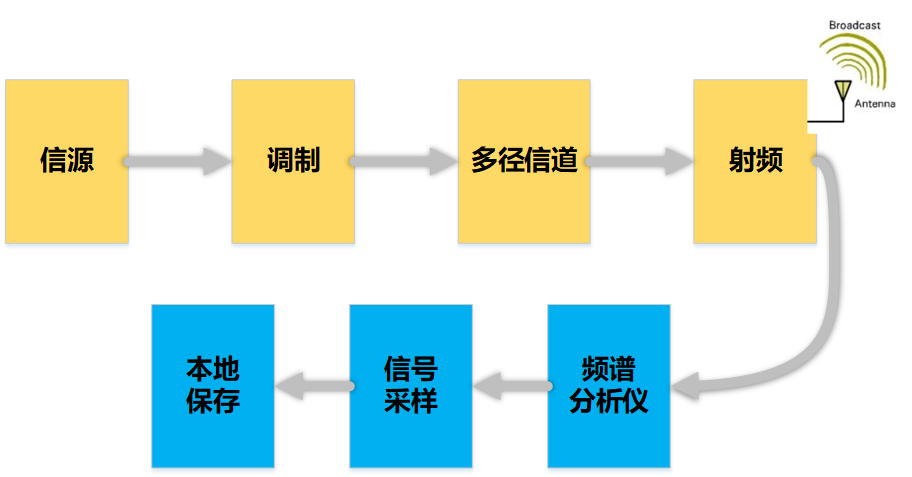
\includegraphics[scale=0.6]{./figures/chapter_3/fig_3_1}
	\caption{调制信号生成框图}\label{sec:fig_3_1}
\end{figure}
最后,我们生成的数据集主要由9种调制方式组成:8类数字调制和1类模拟调制,这些都被广泛应用于我们周围的无线通信系统。
这些调制类别包括BPSK,QPSK,8PSK,16QAM,64QAM,BFSK,CPFSK和PAM4等数字调制方式,以及用于模拟调制的AM-DSB。 
数据以大约每个符号8次采样的速率进行采样,数据源的平均发送功率为0dB。\par


\section{调制信号的表示}

不同的调制信号具有不同的时频特征。本节,我们将原始数据可视化,了解不同信号的时频特征;
同时,我们利用CAE以及CNN获取信号的无监督表示,并展示不同信号在CAE特征空间中的分布状况,
从而进一步了解不同网络框架对调制信号进行特征提取的不同状况。

\subsection{数据集可视化}

对于每一种调制方式,我们随机抽出一个样本,并对其时域(图\ref{sec:fig_3_1})和频域(图\ref{sec:fig_3_2})进行展示。
我们可以发现,不同调制方式之间具备许多相似性,同事也具备一定差异性。有些信号我们是可以通过肉眼进行模糊判别;
但是,受脉冲形变,失真和其他信道影响,有些信号即便是人类专家也很难从视觉上分辨属于何种调制类别。\par

如图(图\ref{sec:fig_3_2})所示,在时域中,我们可以看到XX信号具备较明显的特征,
而XXX特征在视觉上让人感觉像是噪声,很难直接判断出来。\par
\begin{figure}[!h]
	\centering
	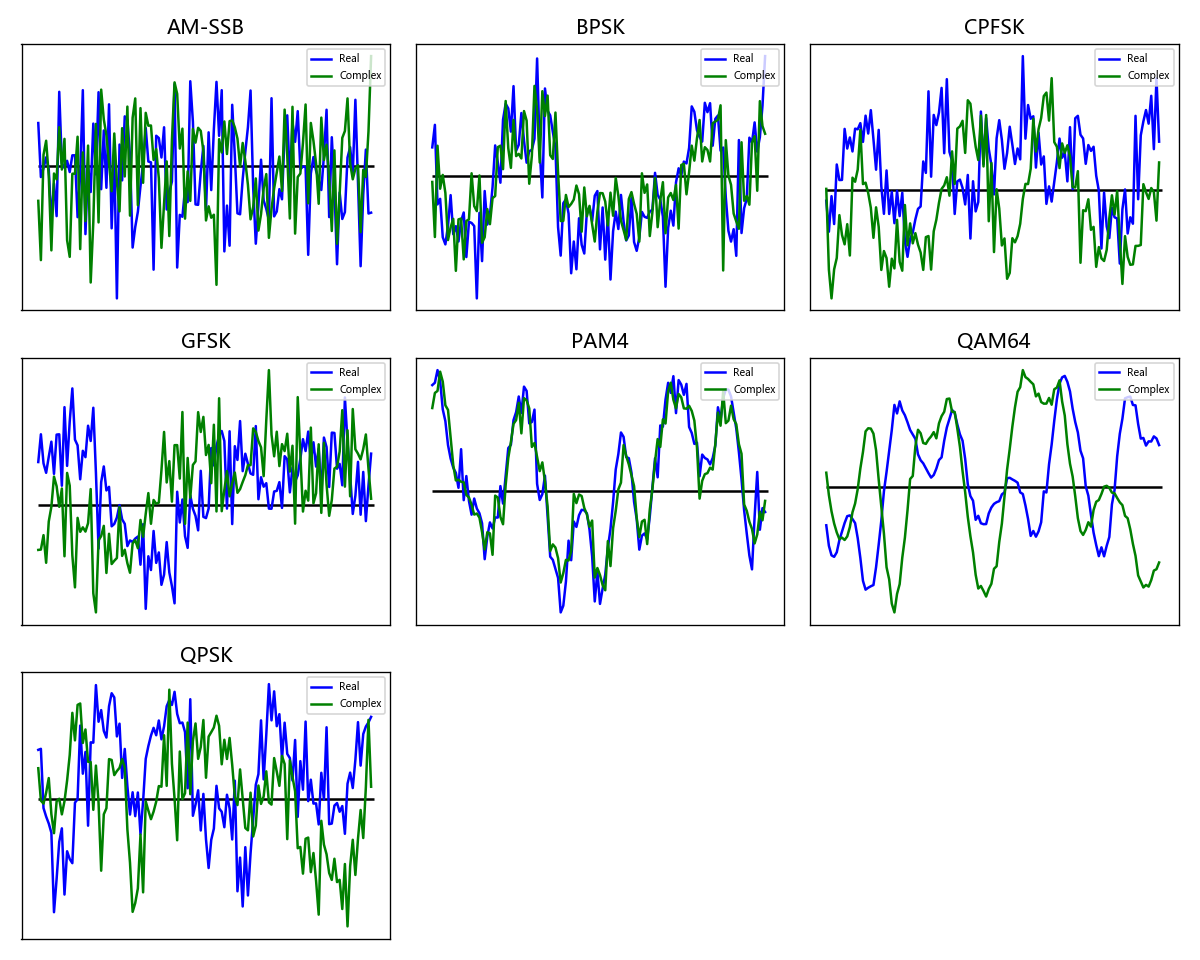
\includegraphics[scale=0.3]{figures/chapter_3/fig_3_2}
	\caption{不同调制方式的高SNR样本的时域波形}\label{sec:fig_3_2}
\end{figure}

如图(图\ref{sec:fig_3_3})所示,在频域中,每一个信号都具备一个带宽限制的功率包络,
其形状为调制识别提供了一定的信息,但是对于人类专家来说,从视觉来说这是一个困难且繁琐的判定方法。\par
\begin{figure}[!h]
	\centering
	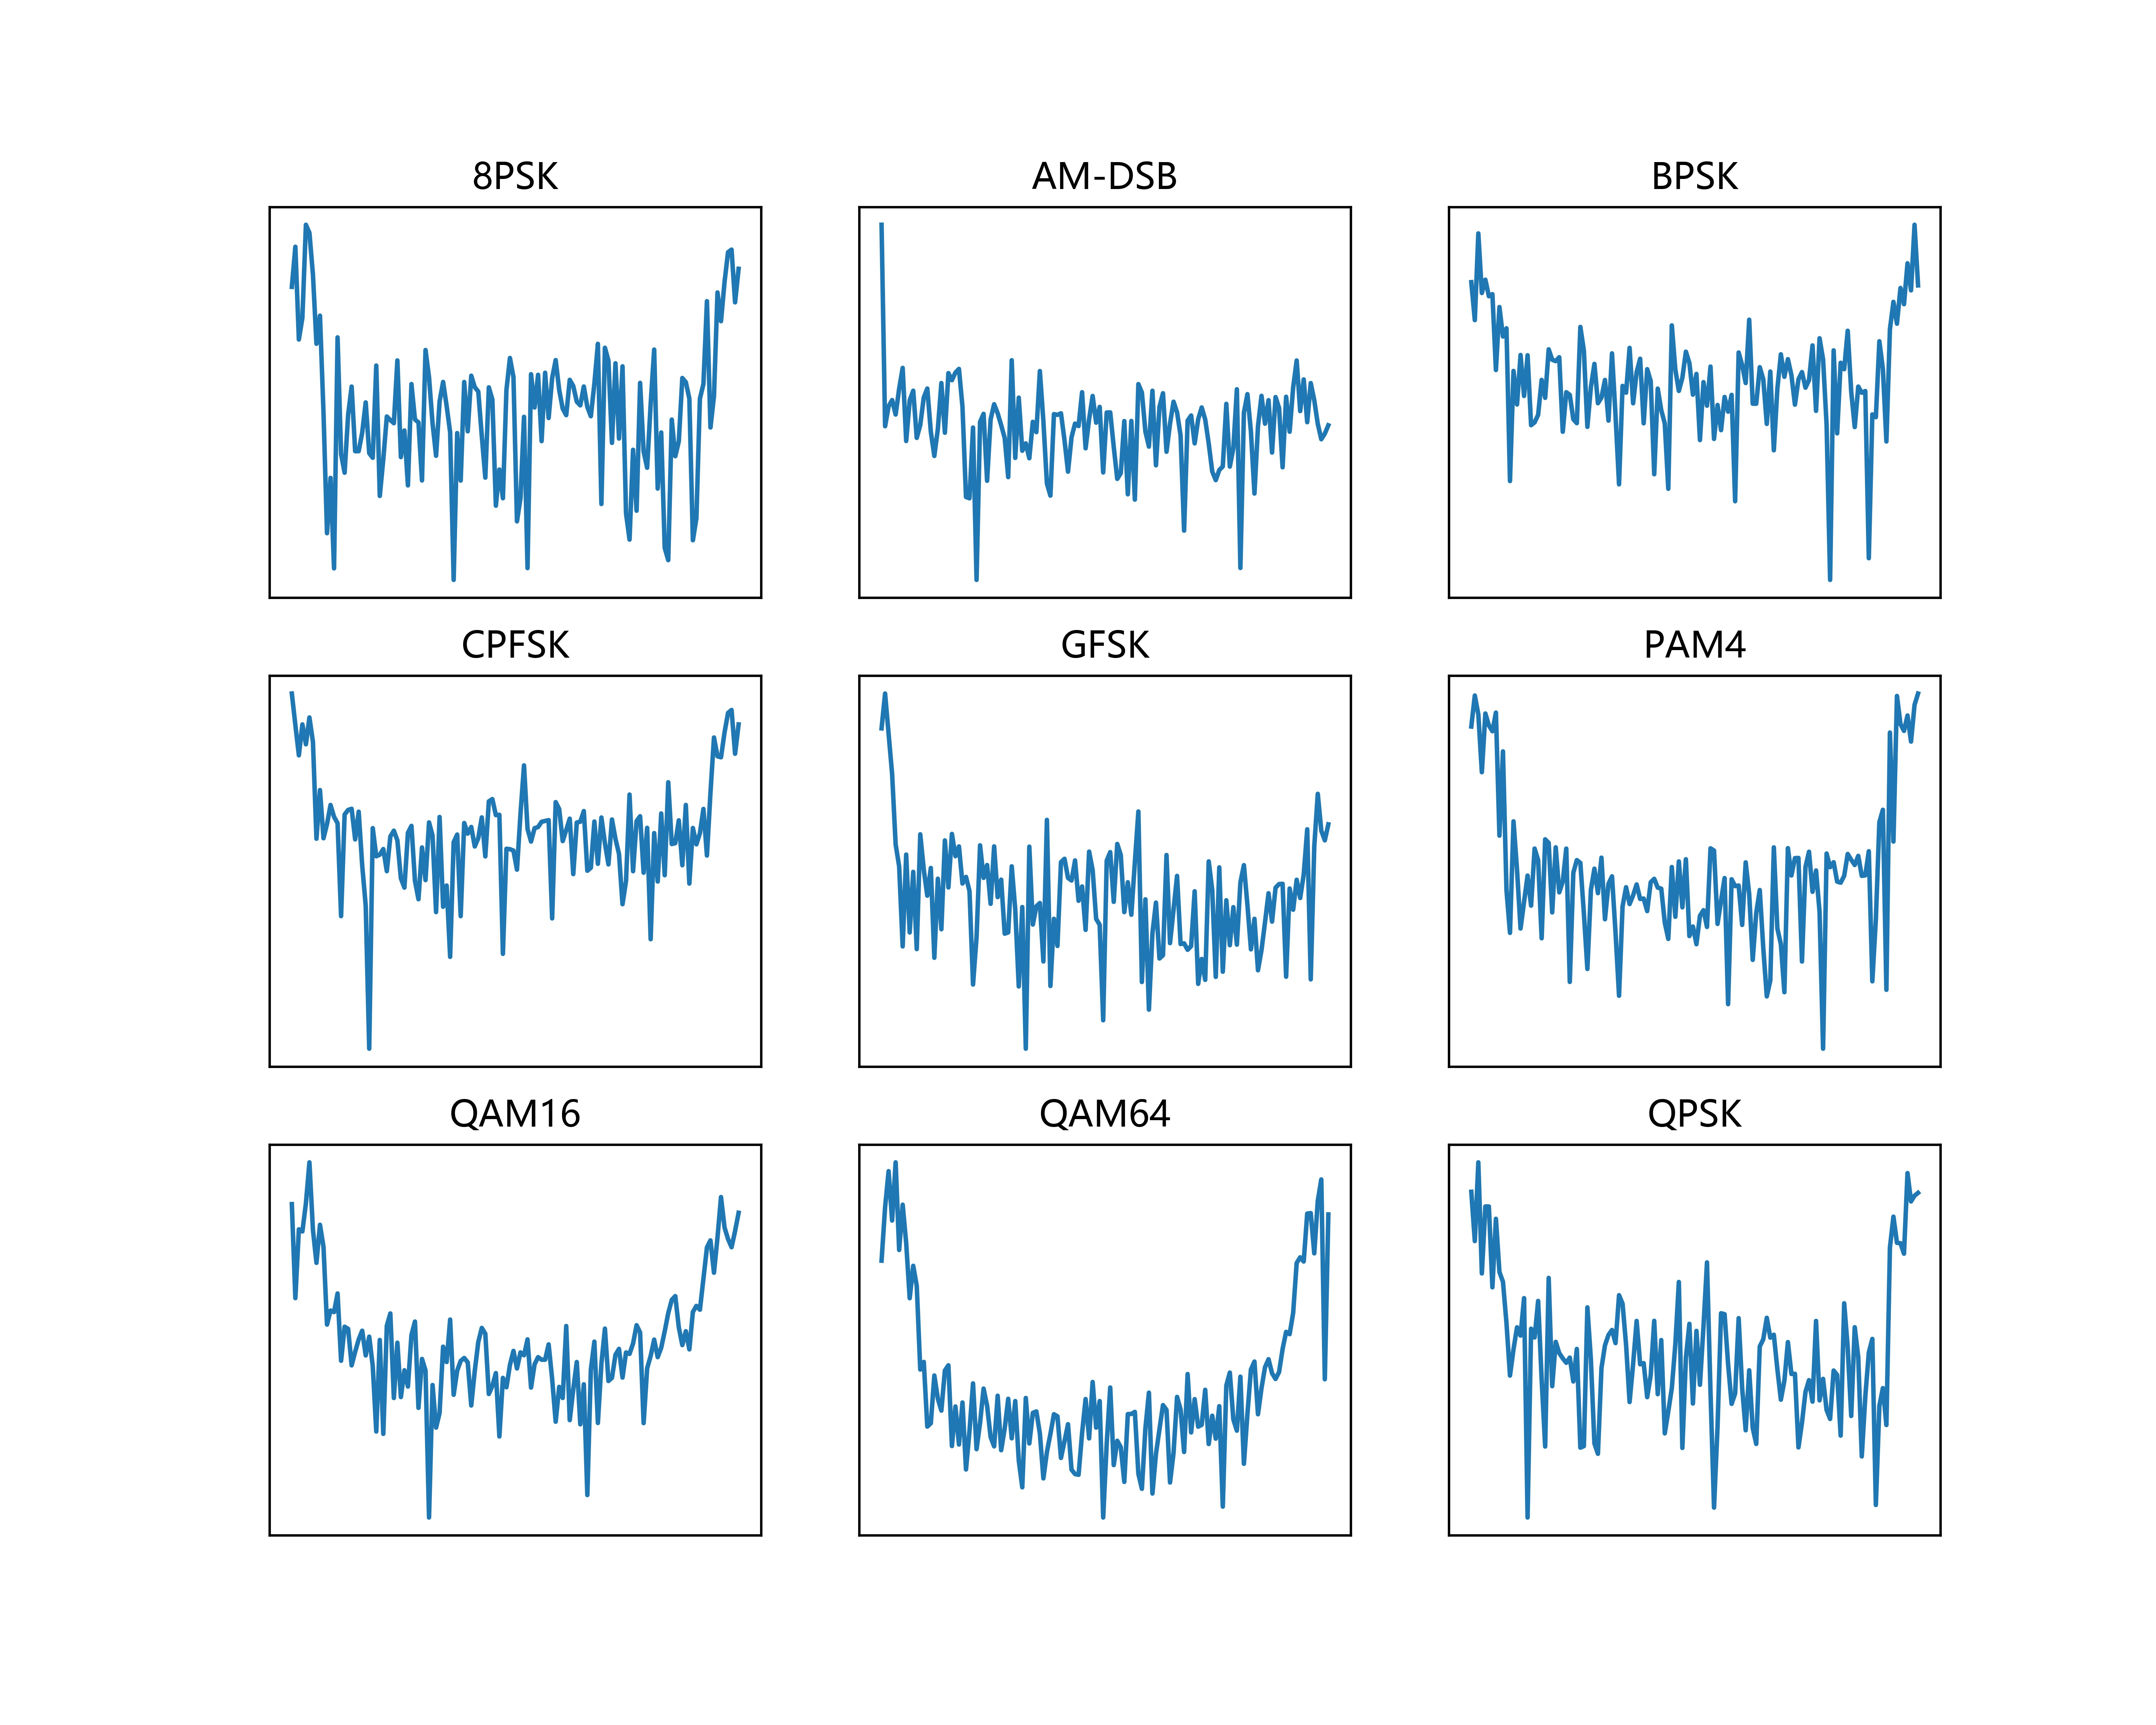
\includegraphics[scale=1.0]{figures/chapter_3/fig_3_3}
	\caption{不同调制方式的高SNR样本的频谱}\label{sec:fig_3_3}
\end{figure}


\subsection{调制信号的无监督表示}

无监督的稀疏表示是指在没有使用类标签的情况下,利用无监督的方法来学习数据集的稀疏表示。
这可以通过使用基于数据依赖性的降维技术来完成,例如主成分分析(PCA)或独立分量分析(ICA)。
但是,这些方法只能对数据进行线性降维,如果说处于低维流型的数据与原始空间本身不具备线性关系,
那么这种情况下就不适合使用线性降维方法。\par

卷积自动编码器(Convolutional Autoencoder,CAE)非常适合于减小参数空间,获取的卷及特征具有时移不变性。
在CAE的训练过程中,我们尽量减少信号重构的均方误差(MSE),但由于我们的主要目标是获得原始信号的聚类稀疏表示,
因此我们对重构误差作出简化假设:限制重构误差最小的情况下尽量降低隐藏层的维度。
然而,由于很难确定重构误差的最小值,
所以,我们只能人为的指定隐层的维度来确定我们的稀疏表示维度,在维度确定的情况下调整参数使重构误差尽量小。
本文中,我们利用卷积自编码器对输入的信号进行重构,学习一组原始信号的非线性稀疏表示。\par
图\ref{sec:fig_3_2}显示了我们的卷积自动编码器使用的体系结构。\par
=======
自动编码器是一种无监督的学习算法,其中神经网络的优化目标是通过一些更有约束的中间维度,使用均方误差(MSE)等损失函数,最小化输出处的重构误差。通常,自编码器利用反向传播算法,将误差进行反向传播,并使用随机梯度下降(SGD)算法等,以找到接近等式\ref{sec:eqt3_3}中的最佳网络参数。

\begin{equation}\label{sec:eqt3_4}
	\mathop{\arg\min}_{\theta}(\sum(X − f (X,\theta))^2)
\end{equation}

通过约束网络的中间层维度,从而可以通过提取用于聚类的中间稀疏编码,来获得原始数据的非线性降维。在这种情况下,使用相似的调制信号,可以由相似的卷积核和特征图来表示,因此,他们分布在该压缩空间的相近区域中。自编码器中的卷积层具有时移不变性以及受约束的参数搜索空间(相对于全连接层),因此非常适合于无线电时间序列信号表示。我们使用dropout[13]并在输入层加入噪声[7]对网络进行正则化,来增强模型的泛化能力。图\ref{fig_3_2}显示了我们的卷积自动编码器使用的体系结构。\par

\begin{figure}[!h]
	\centering
	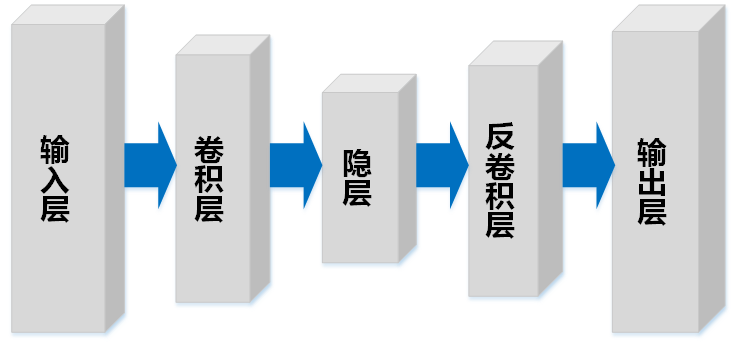
\includegraphics[scale=0.6]{figures/chapter_3/fig_3_4}
	\caption{自编码器}	\label{sec:fig_3_4}
\end{figure}

我们使用RMSProp[11]和Adam[12]梯度下降求解器进行优化,两者都获得了相似的结果,
下文中我们默认使用具备自适应学习速率的Adam优化器进行训练。\par

图\ref{sec:fig_3_5}显示了两个输入维度为$2x128$的训练样本,中间隐层维度为$1x30$,
以及输出维度为$2x128$的训练结果展示图。\par
\begin{figure}[!h]
	\centering
	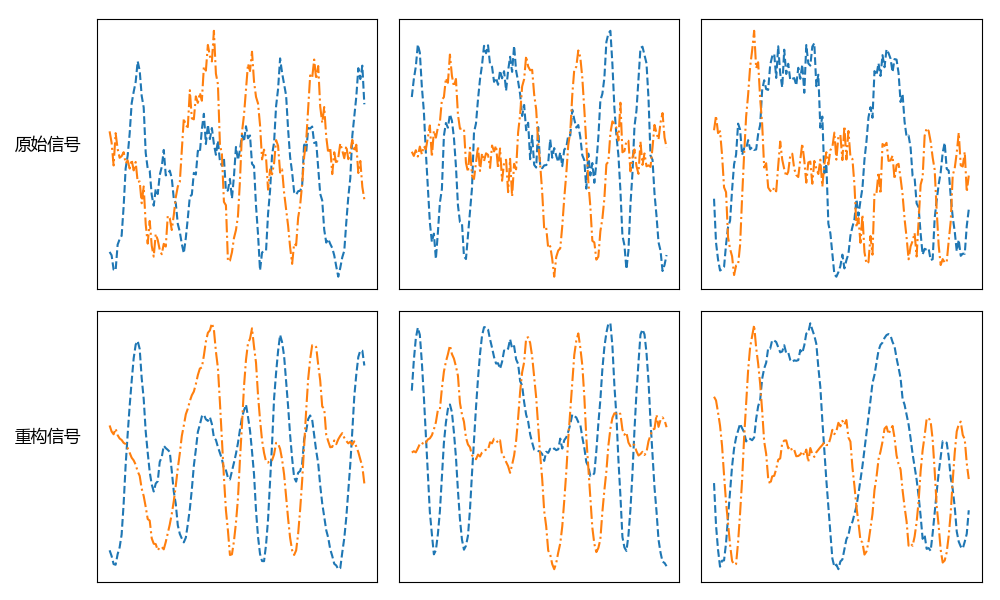
\includegraphics[scale=0.2]{figures/chapter_3/fig_3_5}
	\caption{基于自编码器的信号复现}	\label{sec:fig_3_5}
\end{figure} 

通过图\ref{sec:fig_3_5},我们可以发现,卷积自编码器可以很好的复现原始信号;
我们提取的特征可以很好地重构原始数据,即可以很好地表征原始数据。
这说明我们的卷积自编码器可以通过无监督的方式学习信号的低维嵌入表示。\par

为了可视化我们学到的卷及特征,并对这些特征的类可分性进行直观展示,我们将数据的低维嵌入特征,
利用t-分布随机邻接嵌入(t-asdfasdfa,t-SNE)[6]算法映射到二维流型,并在平面坐标系中展示。
在低维嵌入空间中分布在相近的区域的样本,分布在二维流型中相近的区域。
因此,我们可以通过观察不同类别的数据样本在t-SNE可视化之后的二维流型上的分布,来反映样本无监督表示的类可分性。\par

我们训练卷积自编码器从每一类样本中随机采样100个样本,将其通过训练的卷积自编码器获得其低维无监督表示,
并利用t-SNE映射到二维流型,最终的效果如图X:

\begin{figure}[!h]
	\centering
	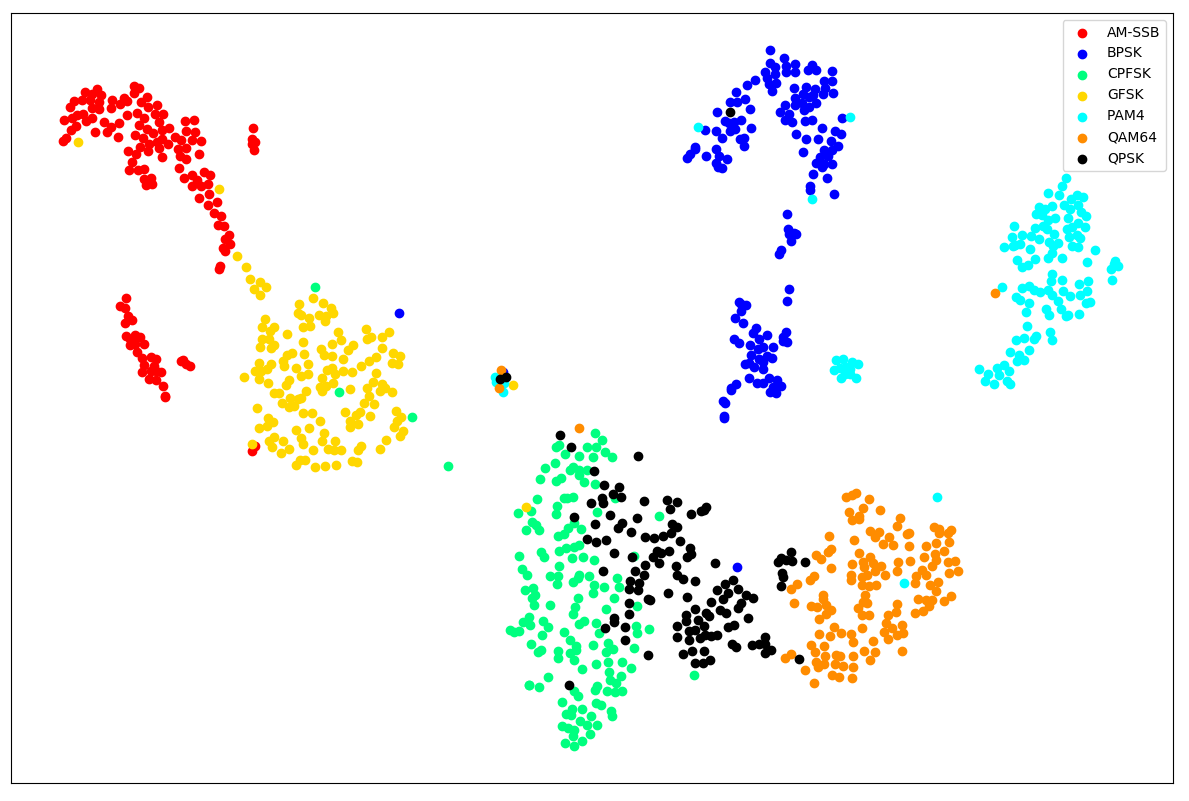
\includegraphics[scale=0.4]{figures/chapter_3/fig_3_6}
	\caption{基于自编码器的调制信号large-vis二维流型展示}	\label{sec:fig_3_6}
\end{figure}

在这种情况下,我们看到几个类如WBFM,AMDSB, AM-SSB和QPSK已经形成了独立的、大部分可分离的簇,
可以利用DBSCAN等聚类方法形成单独的类别;而其他类则会出现类别混淆,并且难以通过聚类方法分离类别簇。 
尽管我们的无监督表示类可分性效果不是很好,但考虑到这些特征从来没有被训练用来区分不同类别的样本,
我们就已经获得了数据一定程度的类可分性,这已经算是一个可以接受的结果了。 \par 

\subsection{调制信号的监督引导稀疏表示}

当我们具有一部分监督数据的时候,我们也可以使用监督训练时学习到的判别特征生成一个稀疏表示空间。
TIM Shead在他的工作[14]中,利用有标记样本以监督方式训练卷积神经网络,可以达到很好的分类效果。
CNN主要是由卷基层与DNN层构成;由于CNN本身可以对测试样本进行分类,这就相当于在进行Softmax层的分类之前,
我们已经获取了原始数据具有类别区分度的特征。
因此,我们可以利用监督的方式,获取原始数据的监督引导特征。\par

在训练好分类网络以后,我们移除最后的softmax层,保留剩余的这一部分网络。
这样,在样本经过训练好的网络,最后隐层输出的特征即为原始数据的稀疏表示。
我们利用监督方式训练网络,并获取监督引导特征空间,获取数据监督引导的稀疏表示。\par
我们从每一类样本中随机采样100个样本,通过图X的网络将其映射到监督引导特征空间,并利用t-SNE映射到二维流型,最终的效果如图X:
\begin{figure}[!h]
	\centering
	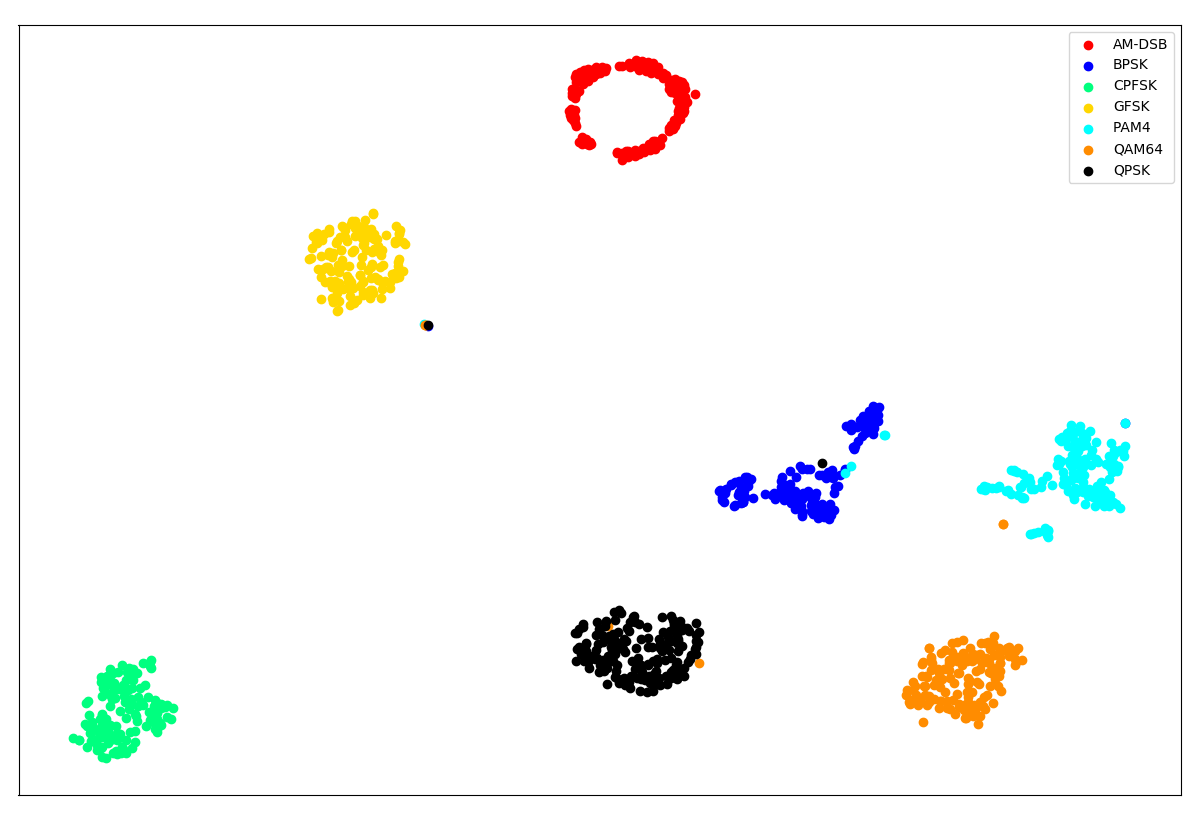
\includegraphics[scale=0.4]{figures/chapter_3/fig_3_7}
	\caption{基于CNN的调制信号large-vis二维流型展示码器}	\label{sec:fig_3_7}
\end{figure}

在这种情况下,我们几乎可以把每个调制类别的样本在二维流型中利用聚类算法分开。
当然,其中也有一部分的数据是混淆的,比如类别X中也有部分样本散落到类别X中。\par
可能是因为在获取监督引导特征空间时,我们的目标是正确区分不同的调制类别,
所以我们获取的监督引导特征对于不同类别的样本是有一定的区分度的,即不同调制类别的样本分布在特征空间的不同区域,
这就表现为在t-SNE之后不同类别样本分布在二维流型的不同区域。
当然,随着训练网络时样本类别的增加,我们获取的具有类区分度的特征将会得到更好的泛化。\par


\section{基于CAE-CNN的无线信号调制识别}

在上一节中,我们分别使用监督引导和无监督引导的方法获取数据的低维表示,其本质上就是基于降维的非线性特征提取过程。
在本节中,通过融合CAE与CNN,我们联合重构误差与分类误差,提出了一种新的调制识别网络框架和算法。

\subsection{CAE-CNN网络框架}
在上一节中,我们发现数据样本在低维嵌入空间中的表示具有一定的类可分性。因此,我们可以将CNN分为特征提取与分类两个步骤。
对于CAE与CNN的融合,我们的本质是希望能够在分类的同时保证特征提取尽量多地包含数据的原始信息。
为此,我们通过在CNN的交叉熵损失中加入CAE的重构误差损失作为我们的整体损失;
通过改进CAE与CNN的训练算法,降低重构误差与分类误差,达到更好的分类效果。
图\ref{sec:fig_3_8}展示了我们网络的结构:

\begin{figure}[!h]
	\centering
	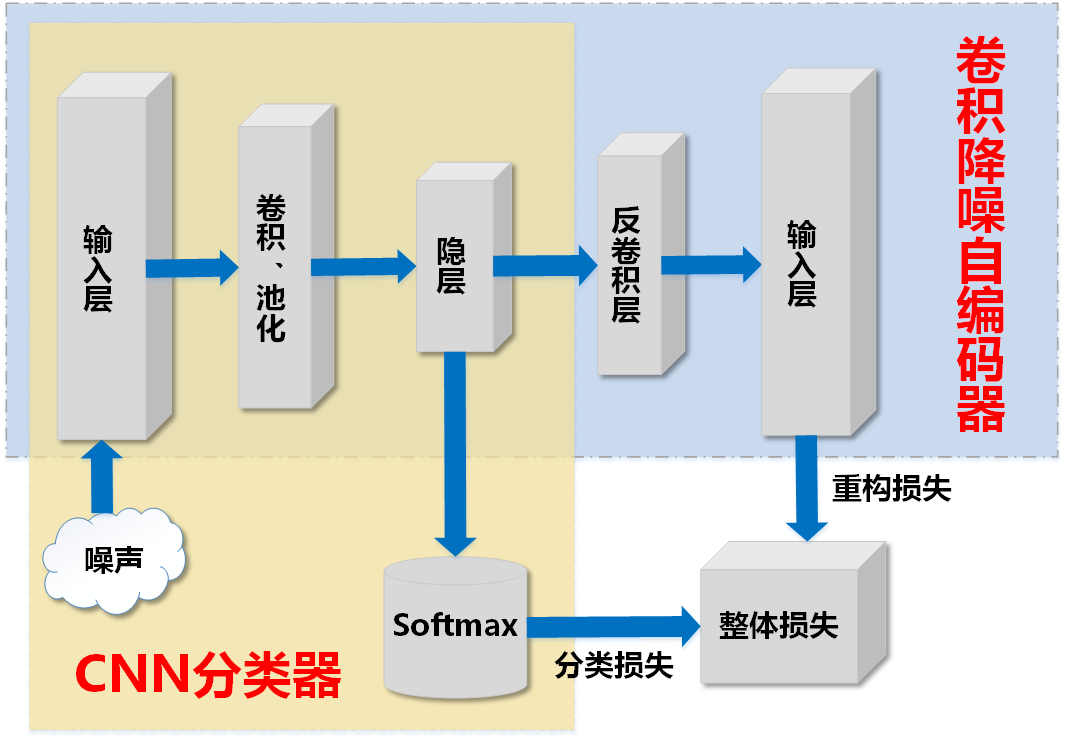
\includegraphics[scale=0.5]{figures/chapter_3/fig_3_8}
	\caption{CAE-CNN网络框架}	\label{sec:fig_3_8}
\end{figure}

在CAE-CNN中的卷基层中,我们使用了Dropout,降低模型的过拟合;
并在卷积权重增加了权重值$W$的2范数作为惩罚项,使权重尽量小;
同时,我们在第一个密集连接层加入权重的$F1$范数范数惩罚来鼓励解的稀疏性[5][10]。\par

那么我们有CAE的损失函数:
\begin{equation}\label{sec:eqt3_3}
r(t) = s(t)*c + n(t)
\end{equation}

由于CNN的损失函数为重构误差与分类误差之和,那么我们有CNN的损失函数:
\begin{equation}\label{sec:eqt3_4}
r(t) = s(t)*c + n(t)
\end{equation}


\subsection{CAE-CNN算法}

\begin{algorithm}[ht]
	\caption{CAE-CNN算法}
	\label{alg:CAE_CNN}
	\begin{algorithmic}
		\REQUIRE 步长 $\epsilon$ (建议默认为: $0.001$)
		\REQUIRE 矩估计的指数衰减速率, $\rho_1$ 和 $\rho_2$ 在区间 $[0, 1)$内。
		(建议默认为:分别为$0.9$ 和 $0.999$)
		\REQUIRE 用于数值稳定的小常数 $\delta$  (建议默认为: $10^{-8}$)
		\REQUIRE 初始参数 $\theta$
		\STATE 初始化一阶和二阶矩变量 $s = 0 $, $r = 0$
		\STATE 初始化\gls{time_step} $t=0$ 
		\WHILE{没有达到停止\gls{criterion}}
		\STATE 从\gls{training_set}中采包含$m$个样本$\{ x^{(1)},\dots, x^{(m)}\}$ 的\gls{minibatch},对应目标为$y^{(i)}$。
		\STATE 计算梯度:$g \leftarrow \frac{1}{m} \nabla_{\theta} \sum_i L(f(x^{(i)};\theta),y^{(i)})$ 
		\STATE $t \leftarrow t + 1$
		\STATE 更新有偏一阶矩估计: $s \leftarrow \rho_1 s + (1-\rho_1) g$
		\STATE 更新有偏二阶矩估计:$r \leftarrow \rho_2 r + (1-\rho_2)  g \odot g$
		\STATE 修正一阶矩的\gls{bias_sta}:$\hat{s} \leftarrow \frac{s}{1-\rho_1^t}$
		\STATE 修正二阶矩的\gls{bias_sta}:$\hat{r} \leftarrow \frac{r}{1-\rho_2^t}$
		\STATE 计算更新:$\Delta \theta = - \epsilon \frac{\hat{s}}{\sqrt{\hat{r}} + \delta}$ \ \  (逐元素应用操作)
		\STATE 应用更新:$\theta \leftarrow \theta + \Delta \theta$
		\ENDWHILE
	\end{algorithmic}
\end{algorithm}


\subsection{算法运行环境及参数}
使用分类交叉熵损失函数和Adam[15]求解器进行训练(在我们的数据集上略胜过RMSProp[12])。
我们在tensorflow[16]计算框架上运行网络的训练和预测,使用Nvidia NVIDIA Cuda[8]组件,
在Nvidia GTX1080ti显卡上加速运算。接下来的仿真我们都使用这一套软硬件组合进行仿真。
我们的机器系统配置如表\ref{sec:table_3_1}所示:\par

\begin{table}[H]
	\centering
	\caption{系统参数配置}
	\begin{tabular}{ccc}
		\toprule
		参数 & 配置\\
		\midrule
		System & Ubuntu 17.10\\
		\midrule
		CPU & Intel\textsuperscript{\textregistered}  Xeon(R) CPU E5-2683 v3 \\
		\midrule
		GPU & GeForce GTX 1080 Ti\\
		\midrule 
		Memory & 64GB\\
		\midrule 
		HardDisk & 1TB\\
		\midrule 
		Python & python3.6\\
		\midrule 
		Library & Tensorflow1.4\\
		\bottomrule
	\end{tabular}
	\label{sec:table_3_1}  
\end{table}

\section{结果及分析}

\subsection{学习复杂度}
我们使用Adam求解器训练了大约23分钟的最高复杂度模型,批量大小为1024的样本训练集大约需要15秒。我们确实观察到一些过度拟合,尽管没有正规化,但验证损失确实 没有显着变化,我们保持最佳的验证损失模型进行评估。\par

绘制学习的特征有时可以让我们直觉了解网络正在学习的底层表示。 在这种情况下,我们在下面绘制卷积层1和卷积层2的滤波器权重。 在图5中,第一层,我们有64个1x3的过滤器。 在这种情况下,我们只需获得一组边缘和梯度检测器,它们在每个I和Q通道上进行操作。\par

在卷积层2中,如图6所示的权重,我们将这个第一层特征图组合成64×16×2×3较大的特征图,其包括在I和Q通道上同时出现的情况。 这些特征图与在包括2D学习边缘检测器和Gabor滤波器的图像转换网络的较低层处所看到的特征图看起来没有太大的不同。\par

\subsection{分类准确率与鲁棒性}
\subsubsection{分类结果}
为了评估分类器的性能,我们看一下测试数据集的分类性能。
我们调制方式总共有11中,每一类调制信号在噪声信噪比为$-20dB~18dB$之间每隔$2dB$进行数据采样,
每个信噪比下采样1000个样本,每个样本共包含128个采样值;
我们将采样值进行希尔伯特变化,这样每个采样值便分为实部与虚部。
我们将80\%的样本作为训练集,10\%的样本作为验证集集,10\%的样本作为测试集。
即训练样本大约有。 这些样本均匀分布在从-20dB到+ 20dB的SNR中,并被标记以便我们可以评估特定子集上的性能。\par
\begin{figure}[!h]
	\centering
	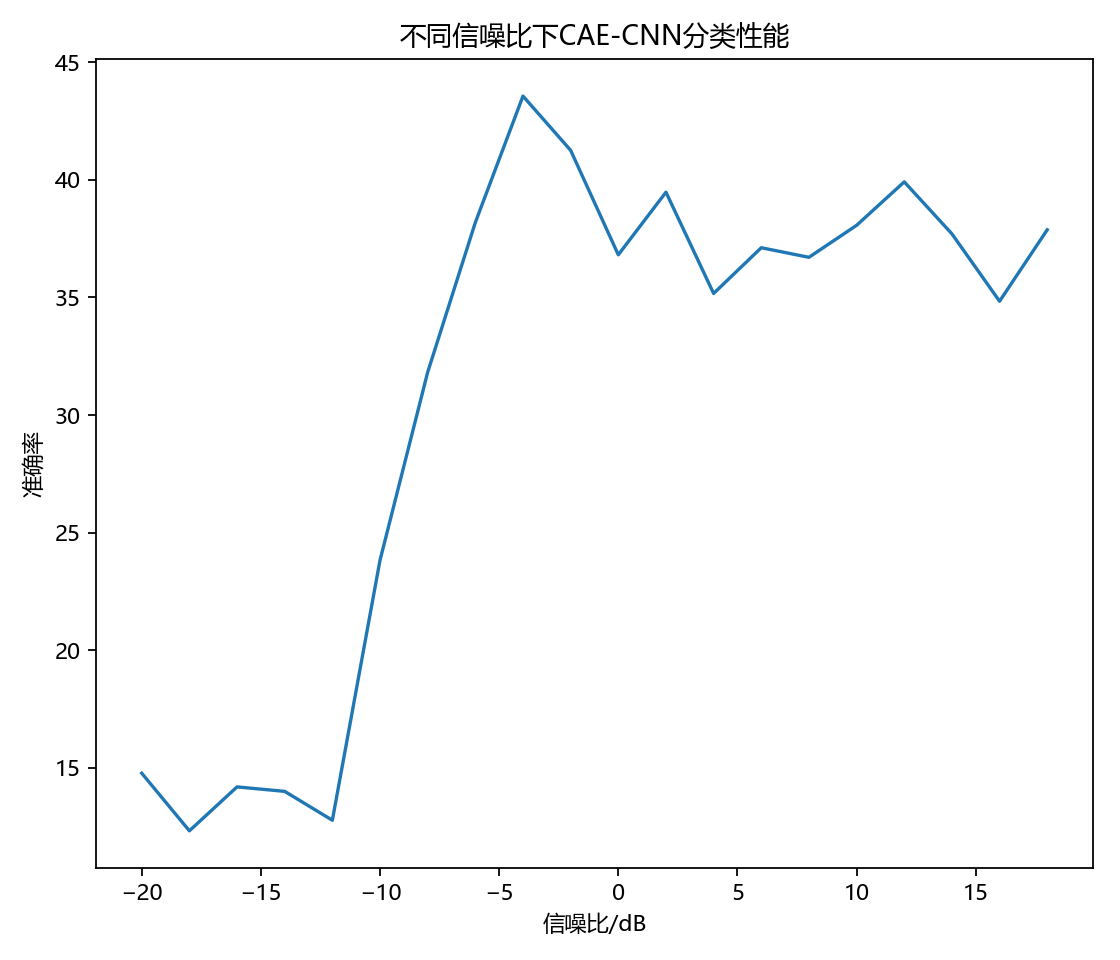
\includegraphics[scale=0.6]{figures/chapter_3/fig_3_9}
	\caption{整体结果}	\label{sec:fig_3_9}
\end{figure}
对于我们最高的SNR情况下的CNN2(0.6)分类,我们在图8中显示了一个混淆矩阵。在+18dBSNR时,在混淆矩阵中我们有一个干净的对角线,可以看到我们剩下的差异是8PSK误分类为QPSK,WBFM误分类作为AM-DSB。这两个都可以在基础数据集中解释。由于QPSK星座点由8PSK点跨越,所以包含特定比特的8PSK符号从QPSK难以分辨。在WBFM /AM-DSB的情况下,模拟语音信号具有只有载波音调存在的静默时段,这使得这些示例不可见。因此,即使在这个数据集的高信噪比下,也不可能获得100%的准确度,并使得重新合理的混淆被合理地容忍。\par
\subsubsection{0dB误分结果}
\begin{figure}[!h]
	\centering
	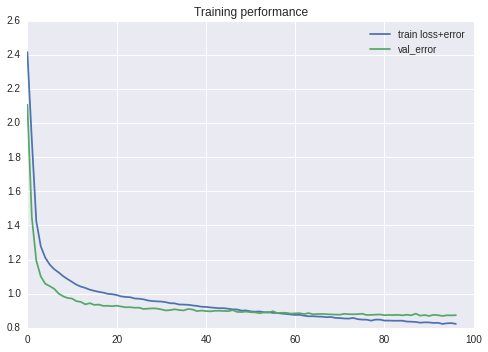
\includegraphics[scale=0.6]{figures/chapter_3/loss}
	\caption{0dB条件下的结果}	\label{sec:fig_3_10}
\end{figure}

\subsubsection{与其他算法的比较}
\begin{figure}[!h]
	\centering
	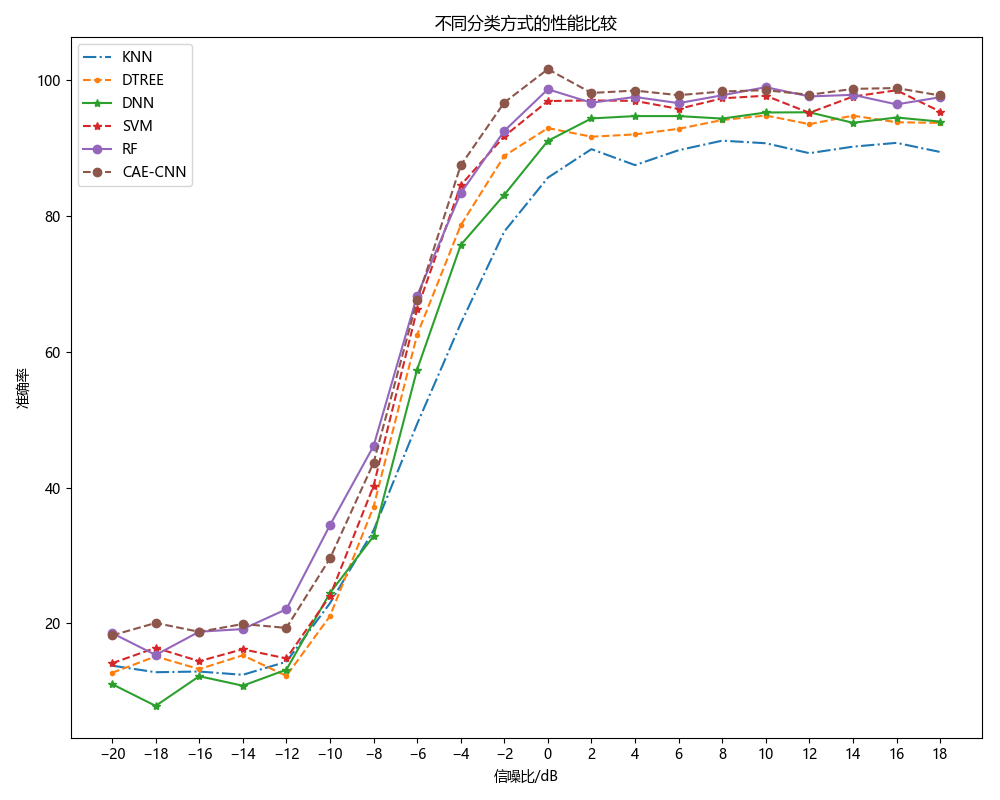
\includegraphics[scale=0.6]{figures/chapter_3/fig_3_11}
	\caption{与其他方法的比较}	\label{sec:fig_3_11}
\end{figure}

在训练之后,我们在测试数据集上的所有信噪比之间的分类准确率大致达到了87.4%,但要理解这个意义,我们必须检查这个分类精度如何在不同训练样本的SNR值之间进行分解,以及 它与现有的基于专家特征的分类器的性能进行比较。绘制测试集调制分类精度,作为每个分类器的示例信噪比的函数7。 实线表示直接在无线电时间序列数据上进行深度特征学习训练的分类器,而虚线表示使用前面描述的专家特征作为输入的分类器。 这种观点是检验结果的关键方法,因为在低信噪比影响范围和覆盖范围的性能,我们可以有效地使用分类器。 我们从具有大量丢失正则化(0.6)的大卷积神经网络(CNN2)中获得显着更好的低SNR分类准确性性能。 在低信噪比情况下,最佳CNN模型的性能比基于专家特征的系统的信噪比高2.5-5dB,而+ 5dB SNR性能相似。 这是一个显着的性能改进,可能至少是传感系统有效覆盖面积的两倍。\par


\subsection{训练效率以及分类效率}

a)训练时间
\begin{figure}[!h]
	\centering
	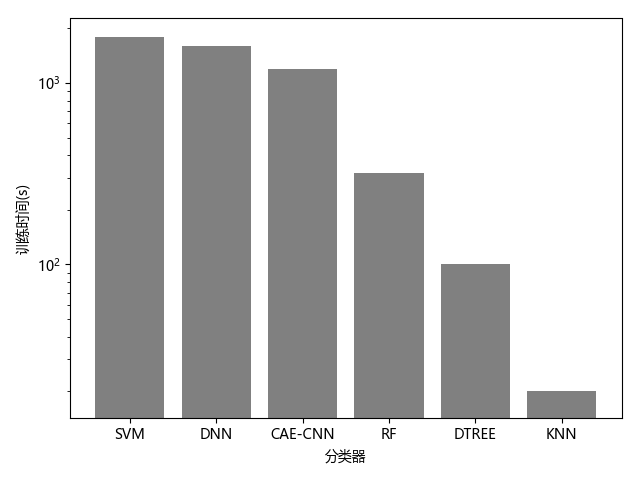
\includegraphics[scale=0.6]{figures/chapter_3/fig_3_12}
	\caption{训练时间}	\label{sec:fig_3_12}
\end{figure}

为了更好地理解性能如何随信噪比而变化,我们检查了不同信噪比级别的几个分类器的混淆矩阵。\par

在非常低的信噪比(-6dB)的情况下,在图9,10,11和12中,我们看到一个有趣的情况,其中±20%内的所有精度都在50%左右。在这种情况下,CNN2分类器上的清洁器对角线比其他3种情况显着更明显,在这个区域学习到的特征具有显着的性能优势。\par

现在,所有4个分类器的信噪比(0dB)略高但仍然很低,现在有一个明确的对角线,但是我们发现在8PSK情况下发生的非对角线误分类更少。\par

b)分类时间

许多无线电系统中的一个重要考虑因素是训练和分类运行时间,由于计算复杂性。 深度学习的一个普遍批评是对大量计算资源的需求,然而在本文中,我们的网络相对紧凑,数据集相对较小。 我们比较下面每个模型的训练和分类运行时间。 在图17中我们可以看到,我们的CNN模型确实需要大量的训练时间,但是比SVM训练案例所需要的时间要少。\par
\begin{figure}[!h]
	\centering
	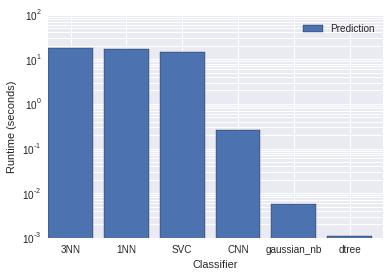
\includegraphics[scale=0.6]{figures/chapter_3/fig_3_13}
	\caption{分类时间}	\label{sec:fig_3_13}
\end{figure}

在图18中显示,使用Tensorflow编译python的这个模型的分类时间比使用scikit-learn的最近邻和SVM模型的大多数其他模型显着更快。只有决策树和GaussianNB模型获得更快的分类运行时间。在这两种情况下,基于ConvNet的这种规模的这种数据集分类模型提出了一个有吸引力的选择这个任务时,分类性能考虑。\par


\section{本章小结}

一旦示例在嵌入空间中形成相对可分的簇,我们可以使用任意数量的聚类算法来将它们中的每一个分组并将其分配给类标签。在图9中,我们展示了一个使用DBSCAN [4]聚类算法的例子,将聚类分成一组未知但不同的调制类。我们发现这种聚类方法比较适合在我们的压缩空间中形成的不明确形状的聚类。聚类之后的数据处理可以包括标记许多示例的集群而不是每个单独的示例,从而提供从数据保存时间的效率提高的数量级。在包含许多类和例子的非常大的数据集上,这使得管理大规模学习任务比其他方法更容易处理。\par
虽然这些集群并非没有错误,但是在这个例子中,通常我们可以找到从发现的类集合到不同的真实命名类的一对一或多对一的映射。这保证了这样一种方法可以在将来用于快速组织和标记大量的无线电发射,并利用关于发射器类别特征的先前知识,但是仍然允许随着时间的推移识别系统能力,特征和类别标签的缩放最大限度地减少这样做所需的人力劳动。\par

虽然这些结果并不是现有的最好的基于专家特征的调制分类器的全面比较,但是它们证明了,与相对专业的被认为的方法相比,时间序列无线电信号数据上的盲卷积网络是可行的并且工作得很好。在图7中,我们比较了几种分类器策略的准确性和信噪比,并且认为对于低信噪比和短时间的示例(128个复杂采样),这代表了调制分类的最先进的精确度方法。这种方法有可能容易地扩展到额外的调制类别,并且应该被视为依赖于无线电发射器的稳健的低SNR分类的DSA和CR系统的有力候选。\par


我们的结果与当前最好的专家系统方法的合理近似相比较,但是由于在无线电领域新兴的机器学习领域不存在强大的竞争数据集,所以很难直接比较性能和当前的现有技术状态。我们希望在以后的工作中进一步评估这一点,并将特征学习和专家方法从目前的水平上进行改进。 CNN2网络体系结构上的性能改进是不可避免的,我们花费了一些努力来优化它,但并没有做到这一点。较大的过滤器,不同的体系结构和池化层可能会显着影响性能,但是在这项工作中没有充分考虑其适用性。许多附加技术可以应用于这个问题,包括引入附加通道引起的效应的不变性,例如膨胀,I / Q不平衡,相位偏移等等。空间变换网络[17]已经证明了学习图像数据的这种不变性的强大能力,并且可以作为一个有趣的候选者,使得能够改善对这些效应的不变性学习。序列模型和递归层[13]可能能够表示信号序列嵌入,并且在更长时间表示中几乎肯定会证明是有价值的,但是我们还没有完全调查这个区域。这个应用领域已经成熟,可以进一步研究和应用,这将大大影响无线信号处理和认知无线电领域的技术发展水平,并将其转向机器学习和数据驱动方法。\par



\chapter{基于传统特征与深度特征融合的无线调制方式识别技术研究}
\section{引言}
图像识别问题是计算机视觉领域要解决的基础问题,如果将图像看作一种模式,那么图像识别问题也是一种特殊的模式分类问题,包括早期的光学字符识别、生物特征识别中的人脸识别、指纹识别、虹膜识别,也包括场景识别、视频中的目标识别、动作识别等. 基于传统的模式分类方法,这类问题已经得到一定程度的解决,例如支持向量机、人工神经网络、近邻法等方法,通过特征提取、分类器训练过程得到分类器,输出分类结果. 但是,传统的模式分类方法通常基于人工设计的特征,经过特征提取算法得到原始图像的特征数据,例如颜色特征、SIFT 特征、HOG 特征、HOF 特征、GIST 特征等,而这些特征数据却存在类内方差较小而类间方差较大的问题.因为一种特征通常只对图像部分特性的变化较为敏感,而对其他特性的变化不敏感,所以,当两类图像的差异在某种特征敏感特性上的差异不大时,基于单一特征训练的分类器就无法输出正确的分类. 除此之外,图像中复杂的背景噪声也会导致特征数据质量下降,既增加分类器训练的难度,又降低分类的准确性.

得到原始图像的特征数据,例如颜色特征、SIFT 特征、HOG 特征、HOF 特征、GIST 特征等,而这些特征数据却存在类内方差较小而类间方差较大的问题.因为一种特征通常只对图像部分特性的变化较为敏感,而对其他特性的变化不敏感,所以,当两类图像的差异在某种特征敏感特性上的差异不大时,基于单一特征训练的分类器就无法输出正确的分类. 除此之外,图像中复杂的背景噪声也会导致特征数据质量下降,既增加分类器训练的难度,又降低分类的准确性.解决这种问题的一种思路就是使用特征融合方法,同时提取多种特征进行分类器训练,实现特征互补,降低单一特征固有缺陷的影响. 特征融合方法的思想来源于早期的信息融合( information fusion)领域,它的数据主要来源于多种传感器,用于军事领域的多传感器融合. 早期信息融合的基础理论主要包括模糊集、证据理论等,后来信息融合在民用领域得到了较快的发展,尤其是在生物安全认证方面[1],进行多生物特征的融合识别. 目前在学术界被公认的信息融合层次划分为分类器级( 决策级) 、特征级和数据级,处理数据的维度和总量依次升高.在模式识别领域,受到计算机运算能力的限制,早期的研究主要集中在分类器级的融合算法,例如,Kittler
等[2]提出的基于贝叶斯决策理论的分类器融合框架,为以后的研究奠定了良好的基础. 近年来,随着人工智能技术的发展,特征融合成为研究热点,特别是在图像识别问题中得到了广泛的应用.

\section{传统特征}
\subsection{基本时频特征}
时间特征\par

频率特征\par

\subsection{高阶累积量}
四阶累积量\par

六阶累积量\par

\subsection{专家循环矩特征}
基于综合循环矩特征[1]目前广泛流行的调制识别和形成分析导出的决策树调制分类到不同的类别。 一般来说,它们采用方程 \ref{subsec:eq1} 给出的形式。
\begin{equation}
	\label{subsec:eq1}
	snm = f_{m}(x^{n}(t)...x^{n}(t + \tau))
\end{equation}
通过计算关于瞬时或时间延迟的接收信号$r(t)$的$n$次方的第$m$阶统计量,我们可以获得一组统计量,该统计量在给定特征的决策过程的情况下将其与其他调制方式唯一地分开。 对于我们的专家功能集,我们计算32个功能。 这些由0和8个样本的循环时间滞后组成。 复数接收信号的前2个功率的前2个时刻,每个时滞的幅度,相位和相位的绝对值。\par

\section{特征融合理论}
特征融合在信息融合中属于中间层次的融合,信息融合理论是特征融合的基础理论.信息融合是对多源异构数据进行综合处理,从而达到联合决策的目的.其实,人类对事物的认知过程就是对多源信息的融合过程[3],人们每时每刻都在通过视觉、听觉、触觉、嗅觉、味觉等多种感官接收各种各样的信息,这些信息转化成了神经脉冲信号传输到大脑皮层进行综合决策.实际应用中,由于多源数据的结构和含义不同,在处理时不能一概而论,必须经过融合算法处理.在计算机视频和模式识别领域,使用特征融合方法解决图像识别问题,就是基于信息融合思想,通过融合算法使用图像多角度、多层次的特征(图像的颜色、形状、梯度)、空间特征和时间特征、全局特征和局部特征等,来实现更智能的图像信息处理.

随着学术研究的推进,信息融合的数据来源更加多样,应用的领域也更加广泛,特别是CPU、GPU计算性能的显著提升,大规模分布式计算、并行计算模型进一步发展,人类能够对大数据进行快速处理,这使得信息融合的研究从分类器级推进到了特征级和数据级的层面.如果将图像识别问题看作模式分类问题,那么使用特征融合方法主要基于2个基本的经验性假设:1) 融合多特征通常比单一特征具有更好的分类性能;2) 进行融合的多种特征之间相关性较小.前者是应用该方法的出发点和基础思想,后者对于图像多特征的选择具有指导意义.应当从多个角度选择相关性尽量小的特征参与特征融合,才能发挥该方法的优点,实现特征互补.特征融合方法直接作用在特征上面,它的优点在于可以直接利用已有的特征提取算法提取特征,相对于重新设计特征和特征提取算法,其花费的代价更低.

模式分类问题的解决过程一般包括数据获取、预处理、特征提取、分类器设计与训练和分类决策等步骤,如图 1所示,信息融合的3个层次恰好可以与这个过程对应.特征保留了必要的、显著的信息,既降低原始数据的冗余性,减少数据噪声,又比分类器决策结果有更充分的数据信息,数据量和数据维度适中,因此在这个层次上进行融合是目前最优的选择.引入特征融合方法的模式分类问题可以表述为,定义模式空间Ω={ω1, ω2, …, ωc}和样本集合X,其中ωk表示一个模式类,X中每个元素Xj是一个样本的特征集合,其中j∈[1, P],P为样本总数;特征集合Xj={Xj1, Xj2, …, XjD}表示样本有D种特征,样本特征向量Xji={xj1i, xj2i, …, xijni}∈Xj,xjnii表示样本第种i特征的一个维度,ni是这种特征的维度,N=∑1D∑1Dni,为样本特征总体维度;基于特征融合的模式分类问题就是得到样本特征集合Xj到ωk的对应关系,记为f:Xj→ωk.

\section{基于深度学习的特征融合算法}
深度学习理论是在人工神经网络的基础上发展起来的机器学习理论,在多层神经网络中加入了更多隐层单元,得到了深度神经网络模型. 其中深度卷积神经网络模型是该理论中的重要模型之一. 使用该模型可以进行有监督地学习,将特征提取过程
与分类器训练过程整合在一起,实现端到端的机器学习. 基于深度学习理论的特征融合算法是将特征融合的思想引入深度神经网络模型,使用多特征输入到模型中进行训练,在模型中选择 2 个隐层进行特征融合.

Simonyan 等[16]首先提出了一种使用双流架构的深度卷积神经网络模型,可解决视频中的动作识别问题. 该模型分别建立一个空间流卷积神经网络和一个时间流卷积神经网络进行独立训练,在最终的 Softmax 分类输出层将这 2 个网络进行融合,属于分类器级的融合. 而 Feichtenhofer 等[15]则在这个基础上改进了网络融合方法,提出了空间特征融合方法和时间特征融合算法,不仅可以在 Softmax 层进行融合,还可以在卷积层之后的 ReLU 层进行融合,实现特征级的融合.
\subsection{空间特征融合算法}
空间特征融合算法可以对卷积层输出的 2 个特征图( feature map) 进行融合,得到融合后的特征图,从而将 2 个深卷积神经网络模型连接在一起,这个连接点就是融合点. 因此,引入特征融合方法之后,2 个深卷积神经网络模型在融合点之前分别进行特征学习,并在融合点将独立学习的特征进行融合,最后开始共同学习. 融合函数定义为
f∶ xa
t + xb
t →yt ( 19)
其中: xat 和 xb
t 表示 t 时刻的视频帧分别经过卷积运算得到的空间特征图,yt 表示融合空间特征图,xa、xb、yt∈RHWD而 H、W 和 D 分别表示特征图的长度、宽度和通道数量. 融合函数包含加性融合函数、最大融合函数、级联融合函数、卷积融合函数和双线性
融合函数等.加性融合函数 ysum = fsum ( xa,xb) ,是对 2 个特征图对应位置元素的值进行相加,如式( 20) 所示,融
合特征图的通道数不变,其中 i∈[1,H],j∈[1,W],d∈[1,D].ysumi,j,d = xa
i,j,d + xbi,j,d ( 20)最大融合函数 ymax = fmax ( xa,xb) 与加性融合函数相似,是将 2 个特征图对应的位置元素值较大的一个作为融合结果,即ymaxi,j,d = max{ xa	i,j,d,xb	i,j,d } ( 21)级联融合函数 ycat = fcat ( xa,xb) 与前两者不同,它保留了 2 个特征图的结果,并将融合后特征图的通道数变为原始特征图的两倍,如ycati,j,2d = xai,j,d,ycat
i,j,2d - 1 = xbi,j,d ( 22)其中 y∈RH × W × 2D.卷积融合函数 yconv = fconv ( xa,xb) ,是将级联融合函数的融合结果与滤波器 f 进行卷积运算,并且引入偏差值 b,从而实现融合特征图的降维处理. 表示为yconv = ycatf + b ( 23)其中 f∈R1 × 1 × 2D × D,b∈RD.

双线性融合函数 ybil = fbil ( xa,xb) ,是对 2 个特征图对应的位置元素进行外积运算后求和,融合特征图的通道数是原始特征图通道数的平方,表示为ybil = ∑Hi = 1∑Wj = 1xaTi,jxbi,j ( 24)其中 ybil∈RD2. 这种融合函数常被用在 ReLU 层,能够对 2 个特征图对应通道进行融合.

\subsection{时间特征融合算法}

时间特征融合算法主要作用在深度卷积神经网络的池化层. 在进行池化处理之前,需要将空间特征图按照时序进行堆叠,使得输入池化层的特征图维度提高,表示为 x1,…,T∈RHWTD. 文献[15]提出了3D 池化方法和 3D 卷积 + 3D 池化方法,直接保留了时序信息.3D 池化方法是对深度卷积神经网络中通常使用的 2D 池化方法的直接扩展,使用 HWT 的 3D 池化立方代替原始池化层的计算方法,对输入的特征图 x进行池化运算,从而将池化处理从空域扩展到时域. 3D 池化立方可以使用最大池化方法,保留立方区域中的最大值作为池化结果. 这种方法是对特征图的单通道进行处理,不进行跨通道的池化运算.3D 卷积 + 3D 池化方法则是在 3D 池化方法基础上,再加入一个滤波器 f∈RH'W'T'DD'和偏差值 b,对输入的特征图 x1,…,T进行卷积运算,如y1,…,T = x1,…,T * f + b ( 25)计算得到的 y1,…,T再进行 3D 池化处理. 使用滤波器 f 可以在一个局部的时空邻域内对图像特征的组合,通过使用H'W'T'D的卷积核进行卷积运算,增加模型的连接权重数量.在处理视频数据时,时间特征融合算法通常与空间特征融合算法同时使用,通过利用视频中的时序信息,提高基于视频的动作识别或者目标识别的准确率.
\section{传统特征与深度特征融合框架}

\subsection{基于LR的融合框架}
\begin{figure}[!h]
	\centering
	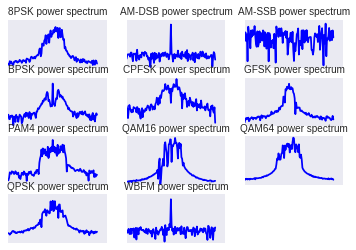
\includegraphics[scale=0.9]{figures/chapter_3/signal_view_2}
	\caption{sigmoid函数与tanh函数}\label{fig_2_2}
\end{figure}

\subsection{基于DNN的融合框架}
\begin{figure}[!h]
	\centering
	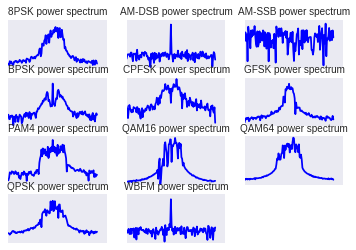
\includegraphics[scale=0.9]{figures/chapter_3/signal_view_2}
	\caption{sigmoid函数与tanh函数}\label{fig_2_2}
\end{figure}

\subsection{基于集成树的融合框架}
\begin{figure}[!h]
	\centering
	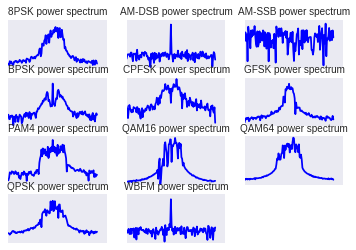
\includegraphics[scale=0.9]{figures/chapter_3/signal_view_2}
	\caption{sigmoid函数与tanh函数}\label{fig_2_2}
\end{figure}


\section{结果及分析}

\begin{figure}[!h]
	\centering
	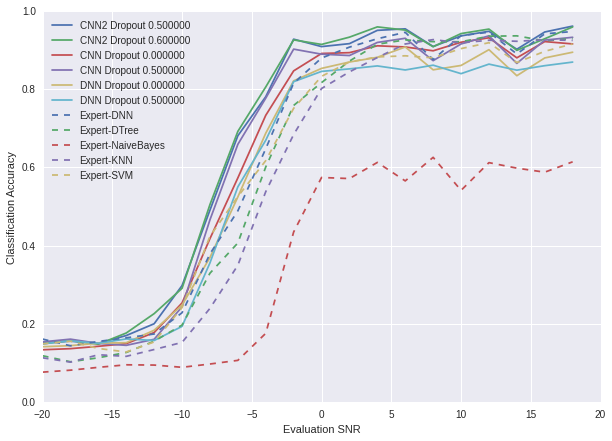
\includegraphics[scale=0.3]{figures/chapter_3/result}
	\caption{sigmoid函数与tanh函数}\label{fig_2_2}
\end{figure}

\subsection{学习概论}
为了验证这一理论,学习歧视性特征可能推广和帮助歧视新的未知调制在半监督的方式使用bootstrap方法,
我们重复我们的先前的方法,但这次我们训练监督分类器11调制9。
我们支持BPSK和16QAM调制,在监督培训期间不提供关于这些类别或其示例的信息。
然后,我们从所有11个类中举例,将它们转换成压缩的特征映射空间,并使用图8中所示的t-SNE可视化二维嵌入。\par

仔细检查这些结果,我们可以看到BPSK不幸与QPSK和8PSK调制(它是其中的一个子集)相当混杂。
然而,QAM16是一个以前看不见的类,这些特征在QAM64附近紧密聚集在一个相当明确的可分离的嵌入空间区域。
这些结果虽然非常初步和定性,但确实支持这一事实,即自举特征映射具有显着的泛化能力,
能够识别,聚类和辨别新的未知的或以前看不见的调制类型,但是并不保证在所有情况下都具有清晰的可分离性。
我们希望随着类别和特征数量的增加,这种泛化将会得到改善。
推进这一研究领域的挑战之一将是确定和量化特征总结能力的衡量标准,并着力于改进这一指标。\par

\subsection{未来应用-聚类}
一旦示例在嵌入空间中形成相对可分的簇,我们可以使用任意数量的聚类算法来将它们中的每一个分组并将其分配给类标签。在图9中,我们展示了一个使用DBSCAN [4]聚类算法的例子,将聚类分成一组未知但不同的调制类。我们发现这种聚类方法比较适合在我们的压缩空间中形成的不明确形状的聚类。聚类之后的数据处理可以包括标记许多示例的集群而不是每个单独的示例,从而提供从数据保存时间的效率提高的数量级。在包含许多类和例子的非常大的数据集上,这使得管理大规模学习任务比其他方法更容易处理。\par
虽然这些集群并非没有错误,但是在这个例子中,通常我们可以找到从发现的类集合到不同的真实命名类的一对一或多对一的映射。这保证了这样一种方法可以在将来用于快速组织和标记大量的无线电发射,并利用关于发射器类别特征的先前知识,但是仍然允许随着时间的推移识别系统能力,特征和类别标签的缩放最大限度地减少这样做所需的人力劳动。\par


\section{本章小结}
在这项工作中,我们已经证明,使用原始采样无线电时间序列数据上的卷积神经网络学习的低级别时间序列特征可以用于有效地聚类许多无线电信号调制类型,而没有明确标记的训练数据。我们已经表明,通过利用从差异特征映射和压缩重构空间学习的压缩表示,我们可以开始组织和构造复杂的无线电信号数据集与未标记或标记不佳的起点。这是一个强有力的结果,因为它展示了一个潜在的前进方向,可以学习区分,推理,回忆和描述新的和未知的无线电信号,而无需手动指导或专家指导。这是一个关键的要求,因为我们试图建立随着时间的推移而从经验中扩展能力的系统。将压缩的特征空间基础推广到新的信号类型仍然是这个领域的一个关键挑战,但是我们在这项工作中已经表明,在某些情况下这种特征泛化确实发生。展望未来,量化和优化这种效应的尝试将是重要的。\par

特征融合方法是模式识别领域的一种重要方法. 计算机视觉领域的图像识别问题作为一种特殊的模式分类
问题,仍然存在很多挑战. 特征融合方法能够综合利用多种图像特征,实现多特征的优势互补,获得更加鲁棒和准
确的识别结果. 笔者基于信息融合理论分析了特征融合方法的原理,介绍了特征融合方法的研究现状,讨论了特征
融合与 3 类主流基础理论相结合的方法,其中基于贝叶斯理论的特征融合算法可以实现多特征的融合决策,基于
稀疏表示理论的特征融合算法能够得到多特征的联合稀疏表示,基于深度学习理论的特征融合算法能够强化深度
神经网络模型的特征学习过程.\par

\chapter{调制识别的深度框架研究}
\section{引言}

有几种完善的网络体系结构,包括多层感知器,卷积网络的许多变体以及循环网络。
 尽管机器学习的目标是开发通用技术,但目前最先进的网络类型似乎仍然是特定于应用程序的。 例如,谷歌认为卷积长短期深度神经网络(CLDNN)值得申请专利,尽管它只用于他们的语音处理研究。 
 图像识别领域的最新技术采用了初始架构,残留网络和其他允许卷积层组合的体系结构的变体,
 同时管理权重和激活的组合复杂性。 \par

我们将深度神经网络应用到无线电调制识别任务中,研究机器学习的最新进展。 结果表明,无线电调制识别不受网络深度的限制,进一步的工作应着重于提高学习的同步和均衡。 这些领域的进步可能来自为这些任务设计的新架构或通过新颖的培训方法。\par

在将深度神经网络应用于无线通信信号之前,值得回顾其他应用领域的现状。下一节将回顾深度神经网络架构和学习进展,这些进展可能对无线通信应用是有效的和有用的。在回顾有趣的深层架构和训练方法之后,结果在第三部分和第四部分讨论。 \par

\subsection{卷积神经网络}

在所有现有技术深度神经网络中的共同元素是卷积层的使用。卷积层由Nf卷积滤波器组成。图像和手写识别开始使用卷积图层来提供特征平移不变性[8]。对于已经熟悉FIR滤波器和DSP的人来说,神经网络中卷积滤波器的使用可能与预期略有不同,至少部分原因是由于神经网络中的激活函数的使用。神经网络中的卷积通常非常小(1x1到5x5是图像处理中的常见尺寸)。在典型的DSP应用中,滤波器非常宽(很多分支/高阶)而非深度(小分支,但是级联)。实现这些滤波器的现代方法(例如多相滤波器组)通常提供了用于由于计算或等待时间原因而减小滤波器宽度的方法。标准卷积层[9]的传递函数在等式3中给出,其中yi是第i个滤波器的输出特征图,b和k代表学习偏差和滤波器权重参数,xi代表输入激活,?表示卷积运算,并且f(::)表示诸如整流线性单元(ReLU)或S形的(通常非线性的)激活函数。。\par

图像处理的神经网络的一个明显趋势是建立更深的网络来学习更复杂的功能和层次特征关系[2],[1]。
深度网络使得可以从原始数据中更容易地学习更复杂的功能,而不是使用相同数量参数的浅层网络[1],[18];
然而,人们普遍认为神经网络中的深度受不稳定梯度的限制,不稳定梯度在网络中的早期层或后期层中爆炸或消失。
近年来,通过在优化器中使用梯度归一化以及不会加剧消失梯度问题的非线性(如整流线性单位(ReLU)),
近年来该问题得到了改善。因此,几个重要的架构已被用于赢得竞争,如ImageNetby增加深度,
我们将着眼于提高无线电调制识别。\par

\subsection{GoogLenet}
GoogLenet [17]中使用的初始架构是一种成功的方法,可以提高网络深度,并能够将不同规模的特性推广到一般管理复杂性。
该网络由重复启动模块组成。每个启动模块(如图1所示)包含四条并行路径,输出是四个并行输出的串联。
第一条路径是一组沿着选定信息转发的1x1卷积。
1x1卷积是一种选择性高速公路网络,它只是简单地向前传递信息而不进行变换。
第二和第三路径是1×1卷积,接着是一组3×3和5×5卷积以提供多个比例的特征检测。
最后,最后的平行路径是一个3x3池化层,接着是1x1卷积。
网络中的中间启动模块连接到softmax分类器,这会导致网络全球培训损失。
这些分类器被认为有助于防止消失梯度。\par

\subsection{ResNet}
增加深度的另一种方法是使用跨层转发信息的体系结构。
迄今为止赢得ImageNet 2015的最佳方法是残余网络[4]。
剩余网络将一层的输出添加到更深层的两层输出中(如图2所示)。
这被称为残留网络,因为转发的信息迫使网络学习残差函数作为特征提取的艺术。 
剩余网络作者认为消失梯度可以通过广泛采用的归一化技术来解决,而深度网络的深度则受限于深度网络的训练复杂度,
这可以通过残差函数来简化。\par


\subsection{CLDNN}
CLDNNs是一种语音处理方法,它可以在原始时域波形上进行操作,而不是专家语音功能,如log-mel cepstrums [16],[15]。 该体系结构使用两个卷积层,随后是两个由长期短期内存(LSTM)单元组成的循环层。 LSTM是一种常见的经常性网络架构,由几个门控制,历史维持多久[5]。 CLDNN也可以具有绕过层的连接,旨在为提取的功能提供更长的时间上下文。 例如,原始CLDNN在LSTM层之前转发具有卷积层输出的原始样本[15]。\par

受使用专业知识指导网络体系结构(如卷积网络和CLDNN)的启发,我们尝试使用卷积网络,我们将其称为卷积匹配滤波器。 相当简单的想法是采用典型通信接收器的通用架构,并构建具有类似部分的神经网络架构。 通信接收机有一个滤波器(通常是采样器),通常前置滤波器抽取每个符号的少量采样,用于执行相移以找到最佳采样点的同步器,然后采样器切片成比特或发射音频以进行模拟调制 。与此类似的神经网络体系结构是一个卷积层,后面跟着一个LSTM。\par


\section{不同框架的识别性能}

\subsection{神经网络训练}


网络的超参数(如学习速率,每层过滤器/特征映射的数量,过滤器大小以及某种程度上的层数)都会影响网络规模并且难以优化。 最近的研究尝试将超参数优化为可以用反向传播和梯度下降(如网络权重和偏差)进行训练的常规参数。 对于这项研究,我们忽略训练超参数,并使用adam优化器[6],它提供梯度归一化和动量,降低超参数的重要性,如学习率。

在工作的指导下,深度比特征图的数量更重要[2],我们将建立一个类似于无线电卷积调制网络[13]中使用的基线卷积网络。 我们的第一步是调整每个滤波器的滤波器数量和抽头数量,并将其视为不重要的超参数,用于余下的实验以测试不同架构对RF数据的适用性。

\subsection{网络参数}
网络的超参数(如学习速率,每层过滤器/特征映射的数量,过滤器的大小以及层的数量)都会影响网络规模,难以优化。最近的研究尝试将超参数优化为可以用反向传播和梯度下降(如网络权重和偏差)进行训练的常规参数。对于这项研究,我们忽略训练超参数,并使用adam优化器[6],它提供了梯度归一化和动量,降低了像学习率这样的超参数的重要性。在工作的指导下,深度比特征图的数量更重要[2],我们将建立一个类似于无线电卷积调制网络[13]中使用的基线卷积网络。我们的第一步是调整每个滤波器的滤波器数量和抽头数量,并将其视为不重要的超参数,用于剩余的实验,以测试不同架构对RF数据的适用性。\par

我们使用RadioML2016.10a数据集[12]作为评估调制识别任务的基础。目标是使用128个样本的复合(基带I / Q)时域矢量来识别11种可能类别中的调制方案。 128个样本以2x128向量馈入网络,其中复数时间样本的实部和虚部被分开。该数据集使用功率延迟分布,频率选择性衰落,本地振荡器偏移和加性高斯白噪声以及这些效应的细节[12]。数据集标有调制类型和SNR地面实况。我们使用全信噪比top-1分类精度作为单一数字基准,并且比较技术显示SNR高于1的精度。\par

所有模型和培训都是通过使用Nano GTX 1070 GPU的theano后端Keras深度学习库完成的。我们从一个类似于CNN2网络的网络开始[13]。这是选择的基线,因为[13]的结果显示专家方法的显着改善;任何进一步的改进应被认为是现有技术。主要区别在于我们将在每个图层上使用大小为1xtaps的滤镜。我们将做一个简单的超参数优化\par

•为RF调制识别找到最佳的滤波器数量和滤波器大小图3:改变每层滤波器的数量具有较小的影响,在较高的SNR下更明显。每个网络在2个卷积层网络中都有1×3的过滤器,有1个致密层和一个softmax分类器。\par

•测试从网络深度和过滤器大小的其他领域获得的假设\par

\subsection{基准卷积网络}

基线卷积网络在softmax分类器之前有两个卷积层和一个致密层。每个隐藏层具有整流线性单元(ReLU)激活功能和50%的丢失。第一个超参数优化是卷积层的大小。每个图层都有1x3的过滤器,我们将改变过滤器的数量来找出需要的数量。从[1],[18],[2]我们预计在过拟合发生之前,过滤器数量的大范围将会给出类似的性能。\par
\begin{figure}[!h]
	\centering
	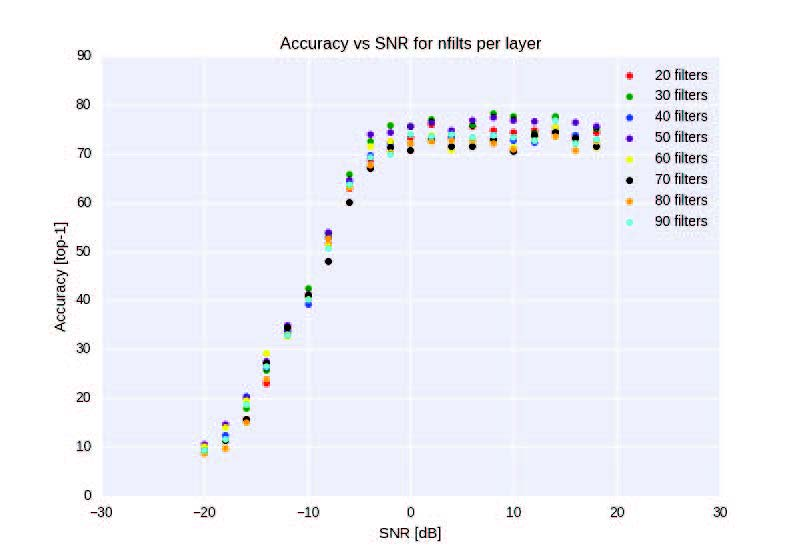
\includegraphics[scale=1]{figures/chapter_5/fig1}
	\caption{图阿斯顿发送到发送}\label{fig_5_1}
\end{figure}
正如所预料的那样,每层大约有30到70个过滤器,而且性能非常相似,这个过滤窗口相当大。对于10-滤波器增量,20-90滤波器的前1分类精度如图1所示。对于其余的实验,我们将使用每层50个滤波器。\par

接下来,我们优化每个过滤器的大小。[2]表明,滤波器的大小也有最小的影响,但基于无线电领域和数据集的专业知识,我们期望8-抽头滤波器是最佳的。对于这个实验,我们使用一个具有单隐藏密集层的双卷积层网络,接着是softmax分类器。卷积层每个都有50个滤波器,其滤波器大小为1xntaps,其中ntaps在3到12之间变化。每个卷积层的滤波器尺寸变化的结果表明,较小的滤波器不如较大的滤波器。我们根据数据集的专家知识假设8抽头滤波器是最好的。图2中每个信噪比图的结果很难区分清楚的赢家;然而,整个数据集分类准确性表明,7-12轻敲都有相似的性能约61%,差异在统计上不显着。\par、

\begin{figure}[!h]
	\centering
	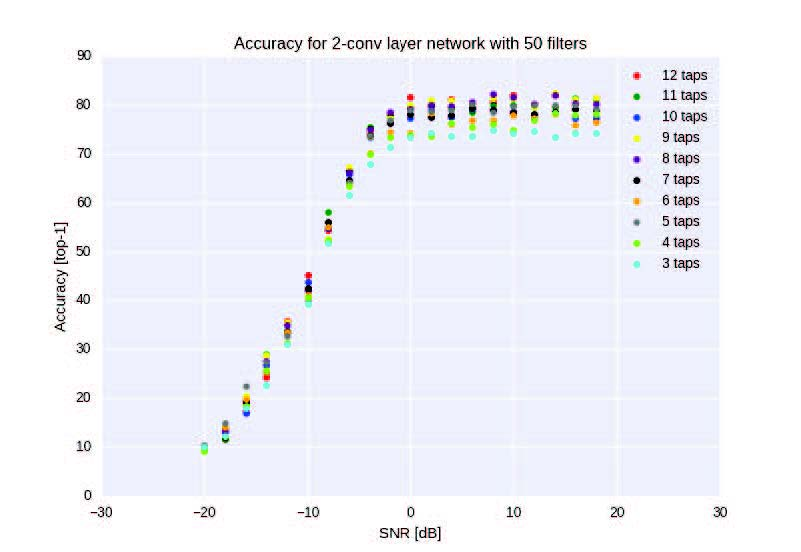
\includegraphics[scale=1]{figures/chapter_5/fig2}
	\caption{改变两个卷积层中的抽头数量(滤波器大小)。水龙头的数量明显较少,但是水龙头的数量增加}\label{fig_5_2}
\end{figure}

最后,对于纯卷积网络,我们尝试增加网络深度。对于这个实验,我们使用1x8滤波器的50抽头卷积层。卷积层之后,我们使用一个隐藏的密集层,然后是最后一个密集的softmax分类器。我们从一个2卷积层网络开始,并添加卷积层。深度学习的趋势表明,增加更多的层次应该改善分类性能,直到梯度变得不稳定。\par

改变卷积层的数目显示很少分类精度没有提高。这个任务的信噪比精度如图3所示。这表明我们的网络没有更多的特征深度学习。由于调制数据通常只改变复数正弦曲线的幅度,频率或相位,所以数据的起始层次不高。

\begin{figure}[!h]
	\centering
	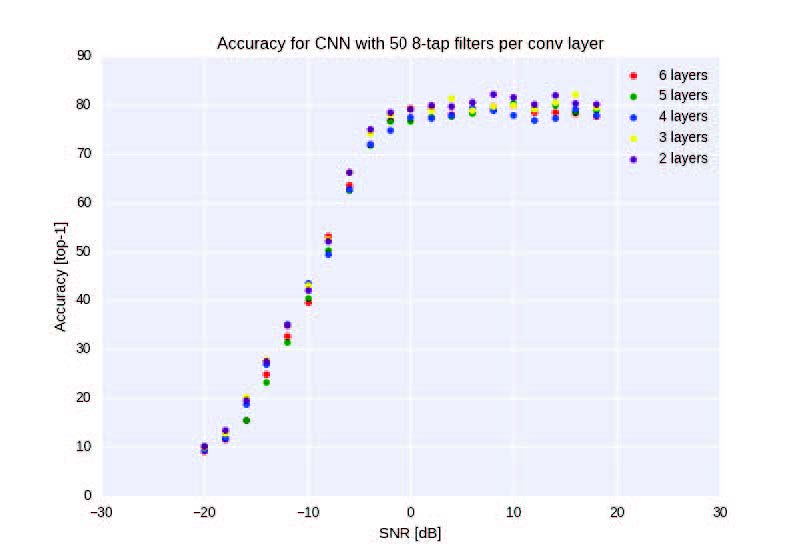
\includegraphics[scale=1]{figures/chapter_5/fig3}
	\caption{改变DNN中的卷积层的数量不会改进无线电调制识别。}
\end{figure}


\subsection{残留网络}

然而,增加更多的卷积层似乎并不能在较低的信噪比下帮助降低噪声的影响。图4显示超参数优化的CNN和9层残留网络的训练损失和验证损失的训练历史记录。这两个网络导致类似的验证损失和训练损失,但剩余的网络在较少的时期训练。\par

\begin{figure}[!h]
	\centering
	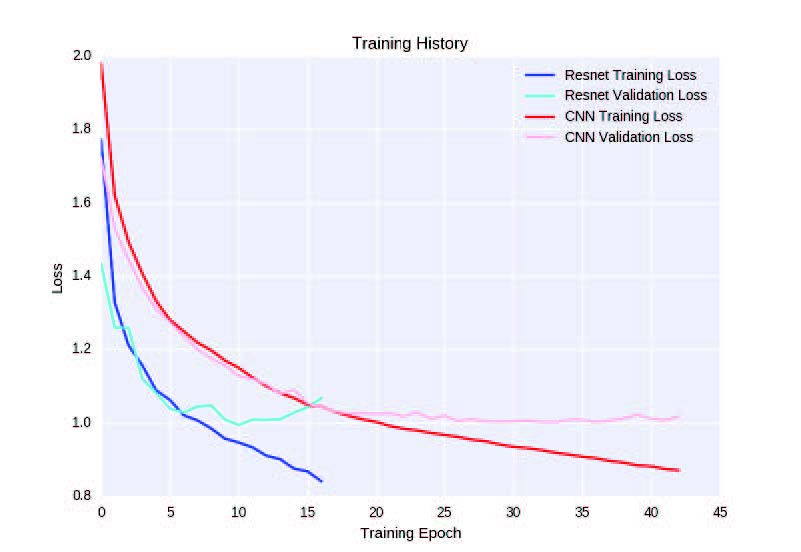
\includegraphics[scale=1]{figures/chapter_5/fig4}
	\caption{显示超参数优化的CNN和9层残留网络的训练损失和验证损失的训练历史记录}
\end{figure}

虽然增加更多的卷积层不会提高分类准确性并不奇怪,但令人惊讶的是,分类和丢失只要2或3个卷积层即可达到平坦。最初的重点是深层网络导致更高的训练损失,这表明更高的训练难度,而不是过度训练。图4显示,我们的超参数优化CNN和9层残留网络达到了相似的损失,验证损失和准确性没有显示;然而,残留网络学习的时间较少。我们还尝试了5-9层的残留网络,这些网络都具有相似的性能和训练时间。这与我们对于普通CNN深度的超参数搜索相结合,表明我们不受无线电学习任务的网络深度限制,尽管我们受到纯粹CNN架构可以学习的特征的限制。\par

先启模块在我们的实验中也没有改进无线电调制分类,使用为我们的数据集调整的初始模块。每个模块使用的三个分支是50个1x1滤波器,50个1x3滤波器和50个1x8滤波器。\par
1x3和1x5滤波器分支前面也有50个1x1滤波器,如图5所示。网络中1-4个初始模块的结果没有显示出超过我们的超参数优化CNN的改进。同样,这表明我们不受深度的限制,也不受限于过滤器的规模。\par

\begin{figure}[!h]
	\centering
	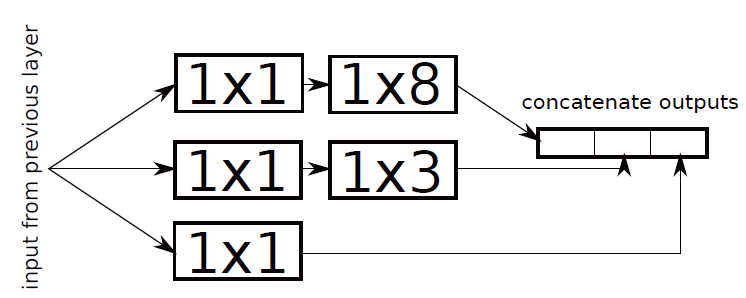
\includegraphics[scale=1]{figures/chapter_5/fig5}
	\caption{用于显示卷积滤波器尺寸的RF数据的初始模块。 每个卷积层有50个过滤器}
\end{figure}

\subsection{CLDNN}

作为我们测试的最终架构,增加了经常性的网络层,即由LSTM单元组成的层,用于对时间特征进行建模。这种方法在时间序列应用中被广泛使用,我们预计调制基带时间序列可能同样适用。我们测试了两层和三层卷积,然后在CLDNNtype体系结构中使用循环层,在循环层之前有和没有正向/旁路连接。我们发现如图6所示的前向连接作为原始波形和卷积输出的连接,导致比其他体系结构更好的分类精度和更稳定的梯度下降。使用会创建类似前面描述的卷积匹配滤波器检测器的结构的合并层不利于分类。\par
\begin{figure}[!h]
	\centering
	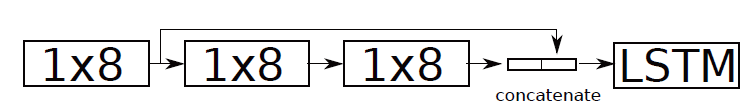
\includegraphics[scale=1]{figures/chapter_5/fig6}
	\caption{用于RF数据的CLDNN体系结构。 在进入LSTM之前,第一个1x8卷积层的输出与三个1x8卷积层的输出级联。}
\end{figure}

\begin{figure}[!h]
	\centering
	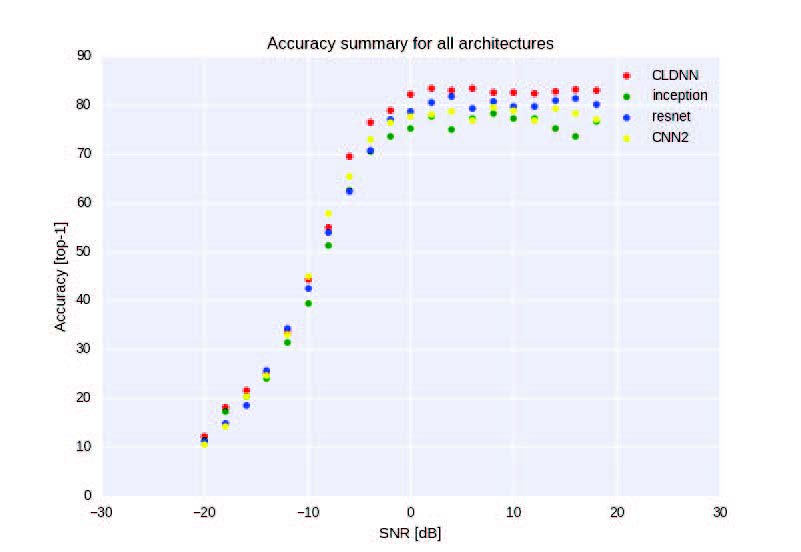
\includegraphics[scale=1]{figures/chapter_5/fig7}
	\caption{CLDNN的信噪比始终优于其他网络架构,信噪比高于-8dB。}
\end{figure}

为了进一步理解什么限制了分类的准确性,我们看一下图8所示的CLDNN的混淆矩阵。有两个主要的混淆领域。一个在模拟调制之间,另一个在高阶QAM之间。模拟调制将很难解决,但是QAM可以在更好的同步和减少信道损伤的情况下得到改善。\par

\begin{figure}[!h]
	\centering
	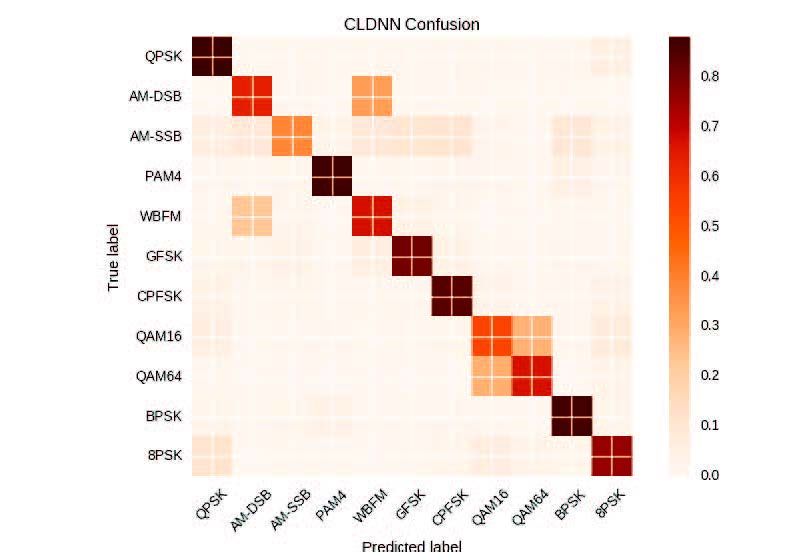
\includegraphics[scale=1]{figures/chapter_5/fig8}
	\caption{CLDNN的全SNR混淆矩阵表明模拟调制与高阶QAM之间的单独混淆之间最混乱。}
\end{figure}

对CLDNN在每一层学习的内容有直观的认识,对于指导未来的工作很重要。为此,我们绘制了一些滤波器抽头的时间和频率表示。对于频率响应,滤波器抽头用100个零填充以获得128点FFT。图9a和10a示出来自第一层的两个选择滤波器。专家的眼睛看起来并不特别熟悉时域表示;然而频率响应确实显示了成形的低通滤波器。未示出的其他滤波器具有频率选择性组件,DC阻断器和类似sinc的频谱形状。\par
\begin{figure}[!h]
	\centering
	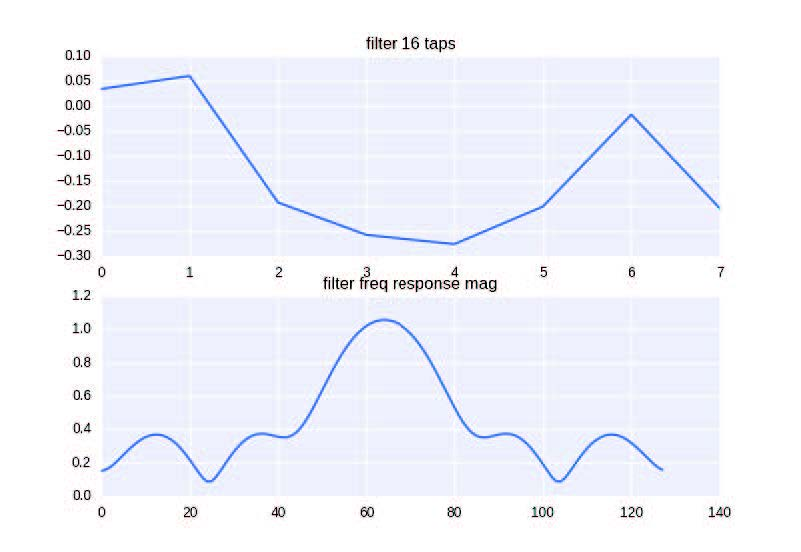
\includegraphics[scale=1]{figures/chapter_5/fig9_a}
	\caption{我们训练的CLDNN的第一卷积层中滤波器的时间和频率幅度表示。。}
\end{figure}
\begin{figure}[!h]
	\centering
	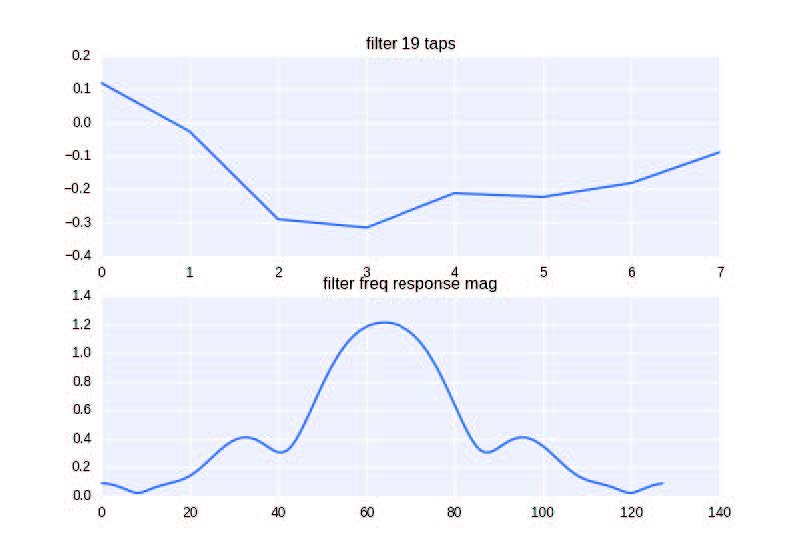
\includegraphics[scale=1]{figures/chapter_5/fig10_a}
	\caption{我们训练的CLDNN的第一卷积层中滤波器的时间和频率幅度表示。。}
\end{figure}

将这些滤波器可视化的另一种方法是将随机数据应用于它们,并对特定滤波器的输出执行梯度上升,该滤波器将收敛于最能激活卷积神经元的数据上[11]。选定的两个过滤器的结果如图9b和10b所示。由此产生的载体看起来有点像粗PSK和FM / FSK调制到专家的眼睛。由于模拟的信道模型,矢量也显示出我们的数据集中存在的一些恒定的相位旋转。需要注意的是,选择这两个过滤器可视化并不是所有的过滤器都对专家有意义。\par

\begin{figure}[!h]
	\centering
	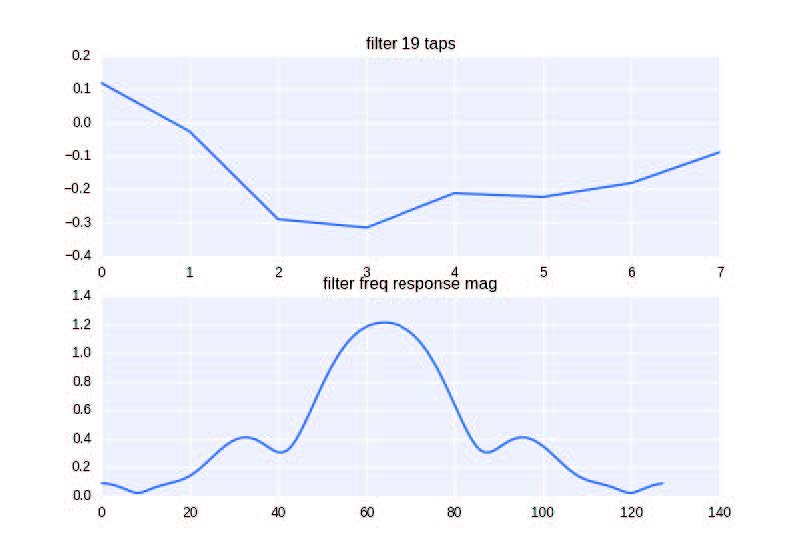
\includegraphics[scale=1]{figures/chapter_5/fig9_b}
	\caption{随机数据训练最大程度地激活过滤器,看起来像BPSK。}
\end{figure}
\begin{figure}[!h]
	\centering
	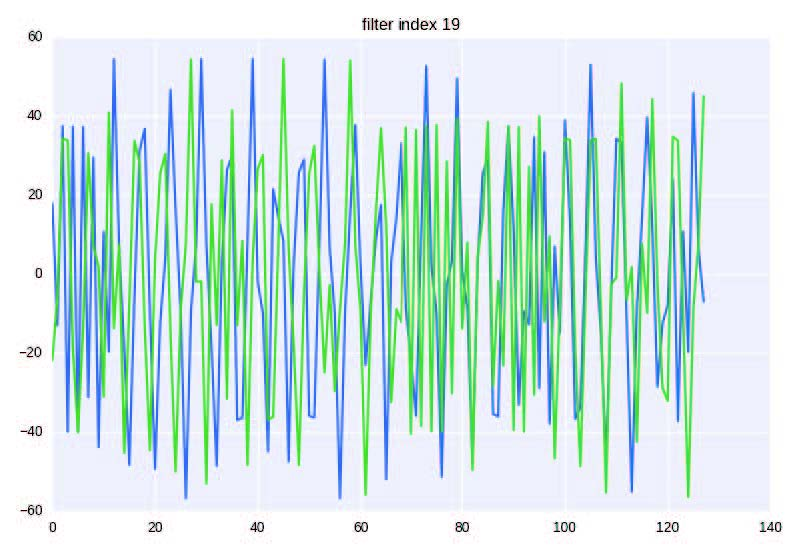
\includegraphics[scale=1]{figures/chapter_5/fig10_b}
	\caption{训练最大程度激活滤波器的随机数据,这看起来像FM或FSK调制。}
\end{figure}

\section{结果及分析}

\section{本章小结}
深度神经网络在无线电领域的性能似乎不受网络深度的限制,就像图像,自然语言处理和声学领域一样。 尽管我们的实验将调制识别作为基准任务,但是我们期望其他无线机器学习任务能够使用类似的网络架构。 无线电任务深度学习的进一步发展可能来自改进的训练方法和网络架构,这些架构可以学习转换射频数据以消除无线信道的影响,这种神经网络架构不是为此设计的。 目前正在探索的一个例子是使用空间变换来均衡和同步输入波形[10]。\par

这些实验还着重于名义上带宽归一化的数据集,这是对从真实无线电传输中捕获的信号的不良假设。 将来在实际应用中使用的网络需要学习对信号进行重新采样以获得带宽规格化,或者学习许多带宽的特性。 可重新采样,同步和消除非线性信道失真的网络都是该领域未来令人兴奋的工作。\par
\chapter{总结与展望}
\section{研究结论}
通信信号调制识别是通信系统中信号解调、信息提取和信号检测的关键技术,因此是一个很有研究价值的课题,近年来取得了很多成果,在电子对抗,软件无线电等领域都有了广泛的应用。在近一年的时间里,查阅了大量的文献,广泛学
习了通信信号调制识别领域的相关研究成果。相对于其它调制识别算法,由于小波变换对瞬时信息具有良好的检测性能,并且在进行通信信号调制类型识别时不需要任何的先验知识,可以在中频上直接对信号进行识别,因此本文针对基于小波变换的调制识别技术进行了深入的研究。下面是本文的主要工作: \par

提出了一套基于小波变换的通信信号调制识别算法。能够在低信噪比条件下直接对所接收到的各种中频数字信号进行识别,与其它同类调制类型算法相比具有较高的识别性能,有一定的实用价值。 对于类间识别,首先,针对传统的基于小波变换幅度信息的调制识别技术进行研究,分析其不足及在低信噪条件下识别率低的问题。然后,提出了一种利用信号包络方差和小波变换频率信息的类间识别算法:首先,利用信号包络的方差分类 MQAM 信号和 MFSK、MPSK 信号,然后采用最优尺度对信号进行小波变换,再提取小波变换相位信息,第二次采用小波变换从小波变换的相位信息中提取瞬时频率信息,根据所提取的频率信息统计方差特征值以区分 MFSK 信号和 MPSK信号。 \par

对于类内识别,针对传统小波变换算法利用相邻码元处的小波变换幅度信息进行 MPSK 信号识别和码元区间内小波变换幅度信息进行 MFSK 信号识别,在低信噪比条件下受噪声影响显著的问题,提出了利用小波变换后相邻码元对应采样
点的相位差信息对 MPSK 信号进行类内识别,利用小波变换从小波变换相位信息中提取频率信息进行 MFSK 信号的类内识别,经过仿真验证,本文方法在相同仿真条件下,具有较高的识别性能,且稳定性好,实现了低信噪比条件下的调制类型识别。由于不同的 QAM 信号瞬时功率均值归一化后其分布特征具有很大差别,本文利用该特点,对小波变换后的瞬时功率进行均值归一化,以识别不同的 QAM信号。 \par

通信信号调制识别是一项不断发展的技术,新的、更复杂的信号调制方式及通信应用的出现,为其提出了越来越多的挑战,使得该技术领域不断有新的研究成果涌现,具有巨大的潜在研究价值。基于小波变换的数字信号调制识别算法的研究已经比较普遍,但是不论在理论方面还是在应用方面都还存在一些值得研究的问题。由于作者在这方面的研究时间较短,因此还有许多相关的问题需要进一步更深入的研究: \par

在调制识别中,如何充分利用小波变换方法和其它支撑矢量机或神经网络方法的优点,将它们有机结合,进一步提高在各种信噪比下的正确识别率。 \par

\section{未来展望}
本文的算法只是在高斯白噪声条件下进行的,如何在瑞利、多径信道条件下实现调制信号的识别,仍然值得继续深入研究。 随着数字调制技术的发展,新的、更复杂的调制方式不断出现,进一步研究与其它新的调制信号的分类问题等。 
希望今后能把通信信号调制识别技术深入的研究下去,做出自己的贡献。\par
% !Mode:: "TeX:UTF-8"
\newcommand{\argmax}{\arg\max}
\newcommand{\argmin}{\arg\min}
\newcommand{\sigmoid}{\text{sigmoid}}
\newcommand{\norm}[1]{\left\lVert#1\right\rVert}
\newcommand{\Tr}{\text{Tr}}

\newcommand{\Var}{\text{Var}}
\newcommand{\Cov}{\text{Cov}}
\newcommand{\plim}{\text{plim}}
\newcommand{\Tsp}{\top}

% Scala
\newcommand{\Sa}{\mathit{a}}
\newcommand{\Sb}{\mathit{b}}
\newcommand{\Sc}{\mathit{c}}
\newcommand{\Sd}{\mathit{d}}
\newcommand{\Se}{\mathit{e}}
\newcommand{\Sf}{\mathit{f}}
\newcommand{\Sg}{\mathit{g}}
\newcommand{\Sh}{\mathit{h}}
\newcommand{\Si}{\mathit{i}}
\newcommand{\Sj}{\mathit{j}}
\newcommand{\Sk}{\mathit{k}}
\newcommand{\Sl}{\mathit{l}}
\newcommand{\Sm}{\mathit{m}}
\newcommand{\Sn}{\mathit{n}}
\newcommand{\So}{\mathit{o}}
\newcommand{\Sp}{\mathit{p}}
\newcommand{\Sq}{\mathit{q}}
\newcommand{\Sr}{\mathit{r}}
\newcommand{\Ss}{\mathit{s}}
\newcommand{\St}{\mathit{t}}
\newcommand{\Su}{\mathit{u}}
\newcommand{\Sv}{\mathit{v}}
\newcommand{\Sw}{\mathit{w}}
\newcommand{\Sx}{\mathit{x}}
\newcommand{\Sy}{\mathit{y}}
\newcommand{\Sz}{\mathit{z}}

\newcommand{\SA}{\mathit{A}}
\newcommand{\SB}{\mathit{B}}
\newcommand{\SC}{\mathit{C}}
\newcommand{\SD}{\mathit{D}}
\newcommand{\SE}{\mathit{E}}
\newcommand{\SF}{\mathit{F}}
\newcommand{\SG}{\mathit{G}}
\newcommand{\SH}{\mathit{H}}
\newcommand{\SJ}{\mathit{J}}
\newcommand{\SK}{\mathit{K}}
\newcommand{\SI}{\mathit{L}}
\newcommand{\SM}{\mathit{M}}
\newcommand{\SN}{\mathit{N}}
\newcommand{\SO}{\mathit{O}}
\newcommand{\SP}{\mathit{P}}
\newcommand{\SQ}{\mathit{Q}}
\newcommand{\SR}{\mathit{R}}
\newcommand{\ST}{\mathit{T}}
\newcommand{\SU}{\mathit{U}}
\newcommand{\SV}{\mathit{V}}
\newcommand{\SW}{\mathit{W}}
\newcommand{\SX}{\mathit{X}}
\newcommand{\SY}{\mathit{Y}}
\newcommand{\SZ}{\mathit{Z}}



% Vector
\newcommand{\Va}{\boldsymbol{\mathit{a}}}
\newcommand{\Vb}{\boldsymbol{\mathit{b}}}
\newcommand{\Vc}{\boldsymbol{\mathit{c}}}
\newcommand{\Vd}{\boldsymbol{\mathit{d}}}
\newcommand{\Ve}{\boldsymbol{\mathit{e}}}
\newcommand{\Vf}{\boldsymbol{\mathit{f}}}
\newcommand{\Vg}{\boldsymbol{\mathit{g}}}
\newcommand{\Vh}{\boldsymbol{\mathit{h}}}
\newcommand{\Vi}{\boldsymbol{\mathit{i}}}
\newcommand{\Vj}{\boldsymbol{\mathit{j}}}
\newcommand{\Vk}{\boldsymbol{\mathit{k}}}
\newcommand{\Vl}{\boldsymbol{\mathit{l}}}
\newcommand{\Vm}{\boldsymbol{\mathit{m}}}
\newcommand{\Vn}{\boldsymbol{\mathit{n}}}
\newcommand{\Vo}{\boldsymbol{\mathit{o}}}
\newcommand{\Vp}{\boldsymbol{\mathit{p}}}
\newcommand{\Vq}{\boldsymbol{\mathit{q}}}
\newcommand{\Vr}{\boldsymbol{\mathit{r}}}
\newcommand{\Vs}{\boldsymbol{\mathit{s}}}
\newcommand{\Vt}{\boldsymbol{\mathit{t}}}
\newcommand{\Vu}{\boldsymbol{\mathit{u}}}
\newcommand{\Vv}{\boldsymbol{\mathit{v}}}
\newcommand{\Vw}{\boldsymbol{\mathit{w}}}
\newcommand{\Vx}{\boldsymbol{\mathit{x}}}
\newcommand{\Vy}{\boldsymbol{\mathit{y}}}
\newcommand{\Vz}{\boldsymbol{\mathit{z}}}

% Matrix
\newcommand{\MA}{\boldsymbol{\mathit{A}}}
\newcommand{\MB}{\boldsymbol{\mathit{B}}}
\newcommand{\MC}{\boldsymbol{\mathit{C}}}
\newcommand{\MD}{\boldsymbol{\mathit{D}}}
\newcommand{\ME}{\boldsymbol{\mathit{E}}}
\newcommand{\MF}{\boldsymbol{\mathit{F}}}
\newcommand{\MG}{\boldsymbol{\mathit{G}}}
\newcommand{\MH}{\boldsymbol{\mathit{H}}}
\newcommand{\MI}{\boldsymbol{\mathit{I}}}
\newcommand{\MJ}{\boldsymbol{\mathit{J}}}
\newcommand{\MK}{\boldsymbol{\mathit{K}}}
\newcommand{\ML}{\boldsymbol{\mathit{L}}}
\newcommand{\MM}{\boldsymbol{\mathit{M}}}
\newcommand{\MN}{\boldsymbol{\mathit{N}}}
\newcommand{\MO}{\boldsymbol{\mathit{O}}}
\newcommand{\MP}{\boldsymbol{\mathit{P}}}
\newcommand{\MQ}{\boldsymbol{\mathit{Q}}}
\newcommand{\MR}{\boldsymbol{\mathit{R}}}
\newcommand{\MS}{\boldsymbol{\mathit{S}}}
\newcommand{\MT}{\boldsymbol{\mathit{T}}}
\newcommand{\MU}{\boldsymbol{\mathit{U}}}
\newcommand{\MV}{\boldsymbol{\mathit{V}}}
\newcommand{\MW}{\boldsymbol{\mathit{W}}}
\newcommand{\MX}{\boldsymbol{\mathit{X}}}
\newcommand{\MY}{\boldsymbol{\mathit{Y}}}
\newcommand{\MZ}{\boldsymbol{\mathit{Z}}}


%Tensor
\newcommand{\TSA}{\textsf{\textbf{A}}}
\newcommand{\TSB}{\textsf{\textbf{B}}}
\newcommand{\TSC}{\textsf{\textbf{C}}}
\newcommand{\TSD}{\textsf{\textbf{D}}}
\newcommand{\TSE}{\textsf{\textbf{E}}}
\newcommand{\TSF}{\textsf{\textbf{F}}}
\newcommand{\TSG}{\textsf{\textbf{G}}}
\newcommand{\TSH}{\textsf{\textbf{H}}}
\newcommand{\TSI}{\textsf{\textbf{I}}}
\newcommand{\TSJ}{\textsf{\textbf{J}}}
\newcommand{\TSK}{\textsf{\textbf{K}}}
\newcommand{\TSL}{\textsf{\textbf{L}}}
\newcommand{\TSM}{\textsf{\textbf{M}}}
\newcommand{\TSN}{\textsf{\textbf{N}}}
\newcommand{\TSO}{\textsf{\textbf{O}}}
\newcommand{\TSP}{\textsf{\textbf{P}}}
\newcommand{\TSQ}{\textsf{\textbf{Q}}}
\newcommand{\TSR}{\textsf{\textbf{R}}}
\newcommand{\TSS}{\textsf{\textbf{S}}}
\newcommand{\TST}{\textsf{\textbf{T}}}
\newcommand{\TSU}{\textsf{\textbf{U}}}
\newcommand{\TSV}{\textsf{\textbf{V}}}
\newcommand{\TSW}{\textsf{\textbf{W}}}
\newcommand{\TSX}{\textsf{\textbf{X}}}
\newcommand{\TSY}{\textsf{\textbf{Y}}}
\newcommand{\TSZ}{\textsf{\textbf{Z}}}

% Tensor Element
\newcommand{\TEA}{\textit{\textsf{A}}}
\newcommand{\TEB}{\textit{\textsf{B}}}
\newcommand{\TEC}{\textit{\textsf{C}}}
\newcommand{\TED}{\textit{\textsf{D}}}
\newcommand{\TEE}{\textit{\textsf{E}}}
\newcommand{\TEF}{\textit{\textsf{F}}}
\newcommand{\TEG}{\textit{\textsf{G}}}
\newcommand{\TEH}{\textit{\textsf{H}}}
\newcommand{\TEI}{\textit{\textsf{I}}}
\newcommand{\TEJ}{\textit{\textsf{J}}}
\newcommand{\TEK}{\textit{\textsf{K}}}
\newcommand{\TEL}{\textit{\textsf{L}}}
\newcommand{\TEM}{\textit{\textsf{M}}}
\newcommand{\TEN}{\textit{\textsf{N}}}
\newcommand{\TEO}{\textit{\textsf{O}}}
\newcommand{\TEP}{\textit{\textsf{P}}}
\newcommand{\TEQ}{\textit{\textsf{Q}}}
\newcommand{\TER}{\textit{\textsf{R}}}
\newcommand{\TES}{\textit{\textsf{S}}}
\newcommand{\TET}{\textit{\textsf{T}}}
\newcommand{\TEU}{\textit{\textsf{U}}}
\newcommand{\TEV}{\textit{\textsf{V}}}
\newcommand{\TEW}{\textit{\textsf{W}}}
\newcommand{\TEX}{\textit{\textsf{X}}}
\newcommand{\TEY}{\textit{\textsf{Y}}}
\newcommand{\TEZ}{\textit{\textsf{Z}}}

% Random Scala
\newcommand{\RSa}{\mathrm{a}}
\newcommand{\RSb}{\mathrm{b}}
\newcommand{\RSc}{\mathrm{c}}
\newcommand{\RSd}{\mathrm{d}}
\newcommand{\RSe}{\mathrm{e}}
\newcommand{\RSf}{\mathrm{f}}
\newcommand{\RSg}{\mathrm{g}}
\newcommand{\RSh}{\mathrm{h}}
\newcommand{\RSi}{\mathrm{i}}
\newcommand{\RSj}{\mathrm{j}}
\newcommand{\RSk}{\mathrm{k}}
\newcommand{\RSl}{\mathrm{l}}
\newcommand{\RSm}{\mathrm{m}}
\newcommand{\RSn}{\mathrm{n}}
\newcommand{\RSo}{\mathrm{o}}
\newcommand{\RSp}{\mathrm{p}}
\newcommand{\RSq}{\mathrm{q}}
\newcommand{\RSr}{\mathrm{r}}
\newcommand{\RSs}{\mathrm{s}}
\newcommand{\RSt}{\mathrm{t}}
\newcommand{\RSu}{\mathrm{u}}
\newcommand{\RSv}{\mathrm{v}}
\newcommand{\RSw}{\mathrm{w}}
\newcommand{\RSx}{\mathrm{x}}
\newcommand{\RSy}{\mathrm{y}}
\newcommand{\RSz}{\mathrm{z}}


% Random Vector
\newcommand{\RVa}{\mathbf{a}}
\newcommand{\RVb}{\mathbf{b}}
\newcommand{\RVc}{\mathbf{c}}
\newcommand{\RVd}{\mathbf{d}}
\newcommand{\RVe}{\mathbf{e}}
\newcommand{\RVf}{\mathbf{f}}
\newcommand{\RVg}{\mathbf{g}}
\newcommand{\RVh}{\mathbf{h}}
\newcommand{\RVi}{\mathbf{i}}
\newcommand{\RVj}{\mathbf{j}}
\newcommand{\RVk}{\mathbf{k}}
\newcommand{\RVl}{\mathbf{l}}
\newcommand{\RVm}{\mathbf{m}}
\newcommand{\RVn}{\mathbf{n}}
\newcommand{\RVo}{\mathbf{o}}
\newcommand{\RVp}{\mathbf{p}}
\newcommand{\RVq}{\mathbf{q}}
\newcommand{\RVr}{\mathbf{r}}
\newcommand{\RVs}{\mathbf{s}}
\newcommand{\RVt}{\mathbf{t}}
\newcommand{\RVu}{\mathbf{u}}
\newcommand{\RVv}{\mathbf{v}}
\newcommand{\RVw}{\mathbf{w}}
\newcommand{\RVx}{\mathbf{x}}
\newcommand{\RVy}{\mathbf{y}}
\newcommand{\RVz}{\mathbf{z}}

% Random Matrix
% will be added later
\newcommand{\RMX}{\boldsymbol{\mathrm{X}}}
\newcommand{\RMA}{\boldsymbol{\mathrm{A}}}

\newcommand{\Valpha}{\boldsymbol{\alpha}}
\newcommand{\Vbeta}{\boldsymbol{\beta}}
\newcommand{\Vtheta}{\boldsymbol{\theta}}
\newcommand{\Vlambda}{\boldsymbol{\lambda}}
\newcommand{\VLambda}{\boldsymbol{\Lambda}}
\newcommand{\Vepsilon}{\boldsymbol{\epsilon}}
\newcommand{\Vmu}{\boldsymbol{\mu}}
\newcommand{\VPhi}{\boldsymbol{\Phi}}
\newcommand{\Vsigma}{\boldsymbol{\sigma}}
\newcommand{\VSigma}{\boldsymbol{\Sigma}}
\newcommand{\Vrho}{\boldsymbol{\rho}}
\newcommand{\Vgamma}{\boldsymbol{\gamma}}
\newcommand{\Vomega}{\boldsymbol{\omega}}
\newcommand{\Vpsi}{\boldsymbol{\psi}}
\newcommand{\Vzeta}{\boldsymbol{\zeta}}
\newcommand{\Vone}{\boldsymbol{1}}


\newcommand{\CalB}{\mathcal{B}}
\newcommand{\CalC}{\mathcal{C}}
\newcommand{\CalG}{\mathcal{G}}
\newcommand{\CalH}{\mathcal{H}}
\newcommand{\CalL}{\mathcal{L}}
\newcommand{\CalM}{\mathcal{M}}
\newcommand{\CalN}{\mathcal{N}}
\newcommand{\CalO}{\mathcal{O}}
\newcommand{\CalD}{\mathcal{D}}
\newcommand{\CalU}{\mathcal{U}}
\newcommand{\CalF}{\mathcal{F}}
\newcommand{\CalT}{\mathcal{T}}

% Set
\newcommand{\SetA}{\mathbb{A}}
\newcommand{\SetB}{\mathbb{B}}
\newcommand{\SetD}{\mathbb{D}}
\newcommand{\SetE}{\mathbb{E}}
\newcommand{\SetG}{\mathbb{G}}
\newcommand{\SetL}{\mathbb{L}}
\newcommand{\SetN}{\mathbb{N}}
\newcommand{\SetR}{\mathbb{R}}
\newcommand{\SetS}{\mathbb{S}}
\newcommand{\SetT}{\mathbb{T}}
\newcommand{\SetV}{\mathbb{V}}
\newcommand{\SetX}{\mathbb{X}}
\newcommand{\SetY}{\mathbb{Y}}

% !Mode:: "TeX:UTF-8"
\newglossaryentry{DL}
{
  name=深度学习,
  description={deep learning},
  sort={deep learning},
}

\newglossaryentry{knowledge_base}
{
  name=知识库,
  description={knowledge base},
  sort={knowledge base},
}

\newglossaryentry{ML}
{
  name=机器学习,
  description={machine learning},
  sort={machine learning},
}

\newglossaryentry{ML_model}
{
  name=机器学习模型,
  description={machine learning model},
  sort={machine learning model},
}

\newglossaryentry{ebv}
{
  name=基本单位向量,
  description={elementary basis vectors},
  sort={elementary basis vectors},
}

\newglossaryentry{logistic_regression}
{
  name=逻辑回归,
  description={logistic regression},
  sort={logistic regression},
}

\newglossaryentry{regression}
{
  name=回归,
  description={regression},
  sort={regression},
}

\newglossaryentry{AI}
{
  name=人工智能,
  description={artificial intelligence},
  sort={artificial intelligence},
  symbol={AI}
}

\newglossaryentry{naive_bayes}
{
  name=朴素贝叶斯,
  description={naive Bayes},
  sort={naive Bayes},
}

\newglossaryentry{representation}
{
  name=表示,
  description={representation},
  sort={representation},
}

\newglossaryentry{representation_learning}
{
  name=表示学习,
  description={representation learning},
  sort={representation learning},
}

\newglossaryentry{AE}
{
  name=自编码器,
  description={autoencoder},
  sort={autoencoder},
}

\newglossaryentry{encoder}
{
  name=编码器,
  description={encoder},
  sort={encoder},
}

\newglossaryentry{decoder}
{
  name=解码器,
  description={decoder},
  sort={decoder},
}

\newglossaryentry{MLP}
{
  name=多层感知机,
  description={multilayer perceptron},
  sort={multilayer perceptron},
  symbol={MLP}
}

\newglossaryentry{cybernetics}
{
  name=控制论,
  description={cybernetics},
  sort={cybernetics},
}

\newglossaryentry{connectionism}
{
  name=联结主义,
  description={connectionism},
  sort={connectionism},
}

\newglossaryentry{ANN}
{
  name=人工神经网络,
  description={artificial neural network},
  sort={artificial neural network},
  symbol={ANN}
}

\newglossaryentry{NN}
{
  name=神经网络,
  description={neural network},
  sort={neural network},
}

\newglossaryentry{SGD}
{
  name=随机梯度下降,
  description={stochastic gradient descent},
  sort={stochastic gradient descent},
  symbol={SGD}
}

\newglossaryentry{linear_model}
{
  name=线性模型,
  description={linear model},
  sort={linear model},
}

\newglossaryentry{mode}
{
  name=峰值,
  description={mode},
  sort={mode},
}

\newglossaryentry{unimodal}
{
  name=单峰值,
  description={unimodal},
  sort={unimodal},
}

\newglossaryentry{modality}
{
  name=模态,
  description={modality},
  sort={modality},
}

\newglossaryentry{multimodal}
{
  name=多峰值,
  description={multimodal},
  sort={multimodal},
}

\newglossaryentry{linear_regression}
{
  name=线性回归,
  description={linear regression},
  sort={linear regression},
}

\newglossaryentry{ReLU}
{
  name=整流线性单元,
  description={rectified linear unit},
  sort={rectified linear unit},
  symbol={ReLU}
}

\newglossaryentry{distributed_representation}
{
  name=分布式表示,
  description={distributed representation},
  sort={distributed representation},
}

\newglossaryentry{nondistributed_representation}
{
  name=非分布式表示,
  description={nondistributed representation},
  sort={nondistributed representation},
}

\newglossaryentry{nondistributed}
{
  name=非分布式,
  description={nondistributed},
  sort={nondistributed},
}

\newglossaryentry{hidden_unit}
{
  name=隐藏单元,
  description={hidden unit},
  sort={hidden unit},
}

\newglossaryentry{LSTM}
{
  name=长短期记忆,
  description={long short-term memory},
  sort={long short-term memory},
  symbol={LSTM}
}

\newglossaryentry{DBN}
{
  name=深度信念网络,
  description={deep belief network},
  sort={deep belief network},
  symbol={DBN}
}

\newglossaryentry{RNN}
{
  name=循环神经网络,
  description={recurrent neural network},
  sort={recurrent neural network},
  symbol={RNN}
}

\newglossaryentry{recurrence}
{
  name=循环,
  description={recurrence},
  sort={recurrence},
}

\newglossaryentry{RL}
{
  name=强化学习,
  description={reinforcement learning},
  sort={reinforcement learning},
}

\newglossaryentry{inference}
{
  name=推断,
  description={inference},
  sort={inference},
}

\newglossaryentry{overflow}
{
  name=上溢,
  description={overflow},
  sort={overflow},
}

\newglossaryentry{underflow}
{
  name=下溢,
  description={underflow},
  sort={underflow},
}

\newglossaryentry{softmax}
{
  name=softmax函数,
  description={softmax function},
  sort={softmax function},
}

\newglossaryentry{softmax_chap15}
{
  name=softmax,
  description={softmax},
  sort={softmax},
}

\newglossaryentry{underestimation}
{
  name=欠估计,
  description={underestimation},
  sort={underestimation},
}

\newglossaryentry{overestimation}
{
  name=过估计,
  description={overestimation},
  sort={overestimation},
}

\newglossaryentry{softmax_unit}
{
  name=softmax单元,
  description={softmax unit},
  sort={softmax unit},
}

\newglossaryentry{softmax_chap11}
{
  name=softmax,
  description={softmax},
  sort={softmax},
}

\newglossaryentry{multinoulli}
{
  name=Multinoulli分布,
  description={multinoulli distribution},
  sort={multinoulli distribution},
}

\newglossaryentry{poor_conditioning}
{
  name=病态条件,
  description={poor conditioning},
  sort={poor conditioning},
}

\newglossaryentry{objective_function}
{
  name=目标函数,
  description={objective function},
  sort={objective function},
}

\newglossaryentry{objective}
{
  name=目标,
  description={objective},
  sort={objective},
}

\newglossaryentry{criterion}
{
  name=准则,
  description={criterion},
  sort={criterion},
}

\newglossaryentry{cost_function}
{
  name=代价函数,
  description={cost function},
  sort={cost function},
}

\newglossaryentry{cost}
{
  name=代价,
  description={cost},
  sort={cost},
}

\newglossaryentry{loss_function}
{
  name=损失函数,
  description={loss function},
  sort={loss function},
}

\newglossaryentry{prcurve}
{
  name=PR曲线,
  description={PR curve},
  sort={PR curve},
}

\newglossaryentry{fscore}
{
  name=F分数,
  description={F-score},
  sort={F-score},
}

\newglossaryentry{loss}
{
  name=损失,
  description={loss},
  sort={loss},
}

\newglossaryentry{error_function}
{
  name=误差函数,
  description={error function},
  sort={error function},
}

\newglossaryentry{GD}
{
  name=梯度下降,
  description={gradient descent},
  sort={gradient descent},
}

\newglossaryentry{local_descent}
{
  name=局部下降,
  description={local descent},
  sort={local descent},
}

\newglossaryentry{steepest}
{
  name=最陡下降,
  description={steepest descent},
  sort={steepest descent},
}

\newglossaryentry{GA}
{
  name=梯度上升,
  description={gradient ascent},
  sort={gradient ascent},
}

\newglossaryentry{derivative}
{
  name=导数,
  description={derivative},
  sort={derivative},
}

\newglossaryentry{critical_points}
{
  name=临界点,
  description={critical point},
  sort={critical point},
}

\newglossaryentry{stationary_point}
{
  name=驻点,
  description={stationary point},
  sort={stationary point},
}

\newglossaryentry{local_minimum}
{
  name=局部极小点,
  description={local minimum},
  sort={local minimum},
}

\newglossaryentry{minimum}
{
  name=极小点,
  description={minimum},
  sort={minimum},
}

\newglossaryentry{local_minima}
{
  name=局部极小值,
  description={local minima},
  sort={local minima},
}

\newglossaryentry{minima}
{
  name=极小值,
  description={minima},
  sort={minima},
}

\newglossaryentry{global_minima}
{
  name=全局极小值,
  description={global minima},
  sort={global minima},
}

\newglossaryentry{local_maxima}
{
  name=局部极大值,
  description={local maxima},
  sort={local maxima},
}

\newglossaryentry{maxima}
{
  name=极大值,
  description={maxima},
  sort={maxima},
}

\newglossaryentry{local_maximum}
{
  name=局部极大点,
  description={local maximum},
  sort={local maximum},
}

\newglossaryentry{saddle_points}
{
  name=鞍点,
  description={saddle point},
  sort={saddle point},
}

\newglossaryentry{global_minimum}
{
  name=全局最小点,
  description={global minimum},
  sort={global minimum},
}

\newglossaryentry{partial_derivatives}
{
  name=偏导数,
  description={partial derivative},
  sort={partial derivative},
}

\newglossaryentry{gradient}
{
  name=梯度,
  description={gradient},
  sort={gradient},
}

\newglossaryentry{identifiable}
{
  name=可辨认的,
  description={identifiable},
  sort={identifiable},
}

\newglossaryentry{directional_derivative}
{
  name=方向导数,
  description={directional derivative},
  sort={directional derivative},
}

\newglossaryentry{line_search}
{
  name=线搜索,
  description={line search},
  sort={line search},
}

\newglossaryentry{example}
{
  name=样本,
  description={example},
  sort={example},
}

\newglossaryentry{hill_climbing}
{
  name=爬山,
  description={hill climbing},
  sort={hill climbing},
}

\newglossaryentry{ill_conditioning}
{
  name=病态,
  description={ill conditioning},
  sort={ill conditioning},
}

\newglossaryentry{jacobian}
{
  name=Jacobian,
  description={Jacobian},
  sort={Jacobian},
}

\newglossaryentry{hessian}
{
  name=Hessian,
  description={Hessian},
  sort={Hessian},
}

\newglossaryentry{second_derivative}
{
  name=二阶导数,
  description={second derivative},
  sort={second derivative},
}

\newglossaryentry{curvature}
{
  name=曲率,
  description={curvature},
  sort={curvature},
}

\newglossaryentry{taylor}
{
  name=泰勒,
  description={taylor},
  sort={taylor},
}

\newglossaryentry{second_derivative_test}
{
  name=二阶导数测试,
  description={second derivative test},
  sort={second derivative test},
}

\newglossaryentry{newton_method}
{
  name=牛顿法,
  description={Newton's method},
  sort={Newton's method},
}

\newglossaryentry{second_order_method}
{
  name=二阶方法,
  description={second-order method},
  sort={second-order method},
}

\newglossaryentry{first_order_method}
{
  name=一阶方法,
  description={first-order method},
  sort={first-order method},
}

\newglossaryentry{lipschitz}
{
  name=Lipschitz,
  description={Lipschitz},
  sort={Lipschitz},
}

\newglossaryentry{lipschitz_continuous}
{
  name=Lipschitz连续,
  description={Lipschitz continuous},
  sort={Lipschitz continuous},
}

\newglossaryentry{lipschitz_constant}
{
  name=Lipschitz常数,
  description={Lipschitz constant},
  sort={Lipschitz constant},
}

\newglossaryentry{convex_optimization}
{
  name=凸优化,
  description={Convex optimization},
  sort={Convex optimization},
}

\newglossaryentry{nonconvex}
{
  name=非凸,
  description={nonconvex},
  sort={nonconvex},
}

\newglossaryentry{nume_optimization}
{
  name=数值优化,
  description={numerical optimization},
  sort={numerical optimization},
}

\newglossaryentry{constrained_optimization}
{
  name=约束优化,
  description={constrained optimization},
  sort={constrained optimization},
}

\newglossaryentry{feasible}
{
  name=可行,
  description={feasible},
  sort={feasible},
}

\newglossaryentry{KKT}
{
  name=Karush–Kuhn–Tucker,
  description={Karush–Kuhn–Tucker},
  sort={Karush–Kuhn–Tucker},
  symbol={KKT}
}

\newglossaryentry{generalized_lagrangian}
{
  name=广义Lagrangian,
  description={generalized Lagrangian},
  sort={generalized Lagrangian},
}

\newglossaryentry{generalized_lagrange_function}
{
  name=广义Lagrange函数,
  description={generalized Lagrange function},
  sort={generalized Lagrange function},
}

\newglossaryentry{equality_constraints}
{
  name=等式约束,
  description={equality constraint},
  sort={equality constraint},
}

\newglossaryentry{inequality_constraints}
{
  name=不等式约束,
  description={inequality constraint},
  sort={inequality constraint},
}

\newglossaryentry{regularization}
{
  name=正则化,
  description={regularization},
  sort={regularization},
}

\newglossaryentry{regularizer}
{
  name=正则化项,
  description={regularizer},
  sort={regularizer},
}

\newglossaryentry{regularize}
{
  name=正则化,
  description={regularize},
  sort={regularize},
}

\newglossaryentry{generalization}
{
  name=泛化,
  description={generalization},
  sort={generalization},
}

\newglossaryentry{generalize}
{
  name=泛化,
  description={generalize},
  sort={generalize},
}

\newglossaryentry{underfitting}
{
  name=欠拟合,
  description={underfitting},
  sort={underfitting},
}

\newglossaryentry{overfitting}
{
  name=过拟合,
  description={overfitting},
  sort={overfitting},
}

\newglossaryentry{bias_sta}
{
  name=偏差,
  description={bias in statistics},
  sort={bias in statistics},
}

\newglossaryentry{BIAS}
{
  name=偏差,
  description={biass},
  sort={biass},
}

\newglossaryentry{bias_aff}
{
  name=偏置,
  description={bias in affine function},
  sort={bias in affine function},
}

\newglossaryentry{variance}
{
  name=方差,
  description={variance},
  sort={variance},
}

\newglossaryentry{ensemble}
{
  name=集成,
  description={ensemble},
  sort={ensemble},
}

\newglossaryentry{estimator}
{
  name=估计,
  description={estimator},
  sort={estimator},
}

\newglossaryentry{weight_decay}
{
  name=权重衰减,
  description={weight decay},
  sort={weight decay},
}

\newglossaryentry{ridge_regression}
{
  name=岭回归,
  description={ridge regression},
  sort={ridge regression},
}

\newglossaryentry{tikhonov_regularization}
{
  name=Tikhonov正则,
  description={Tikhonov regularization},
  sort={Tikhonov regularization},
}

\newglossaryentry{covariance}
{
  name=协方差,
  description={covariance},
  sort={covariance},
}

\newglossaryentry{sparse}
{
  name=稀疏,
  description={sparse},
  sort={sparse},
}

\newglossaryentry{feature_selection}
{
  name=特征选择,
  description={feature selection},
  sort={feature selection},
}

\newglossaryentry{feature_extractor}
{
  name=特征提取器,
  description={feature extractor},
  sort={feature extractor},
}

\newglossaryentry{MAP}
{
  name=最大后验,
  description={Maximum A Posteriori},
  sort={Maximum A Posteriori},
  symbol={MAP}
}

\newglossaryentry{pooling}
{
  name=池化,
  description={pooling},
  sort={pooling},
}

\newglossaryentry{dropout}
{
  name=Dropout,
  description={Dropout},
  sort={dropout},
}

\newglossaryentry{monte_carlo}
{
  name=蒙特卡罗,
  description={Monte Carlo},
  sort={Monte Carlo},
}

\newglossaryentry{early_stopping}
{
  name=提前终止,
  description={early stopping},
  sort={early stopping},
}

\newglossaryentry{CNN}
{
  name=卷积神经网络,
  description={convolutional neural network},
  sort={convolutional neural network},
  symbol={CNN}
}

\newglossaryentry{mcmc}
{
  name=马尔可夫链蒙特卡罗,
  description={Markov Chain Monte Carlo},
  symbol={MCMC},
  sort={Markov Chain Monte Carlo},
}

\newglossaryentry{tempering_transition}
{
  name=回火转移,
  description={tempered transition},
  sort={tempered transition},
}

\newglossaryentry{markov_chain}
{
  name=马尔可夫链,
  description={Markov Chain},
  sort={Markov Chain},
}

\newglossaryentry{harris_chain}
{
  name=哈里斯链,
  description={Harris Chain},
  sort={Harris Chain},
}

\newglossaryentry{minibatch}
{
  name=小批量,
  description={minibatch},
  sort={minibatch},
}

\newglossaryentry{importance_sampling}
{
  name=重要采样,
  description={Importance Sampling},
  sort={Importance Sampling},
}

\newglossaryentry{undirected_model}
{
  name=无向模型,
  description={undirected Model},
  sort={undirected Model},
}

\newglossaryentry{partition_function}
{
  name=配分函数,
  description={Partition Function},
  sort={Partition Function},
}

\newglossaryentry{law_of_large_numbers}
{
  name=大数定理,
  description={Law of large number},
  sort={Law of large number},
}

\newglossaryentry{central_limit_theorem}
{
  name=中心极限定理,
  description={central limit theorem},
  sort={central limit theorem},
}

\newglossaryentry{energy_based_model}
{
  name=基于能量的模型,
  description={Energy-based model},
  symbol={EBM},
  sort={Energy-based model},
}

\newglossaryentry{tempering}
{
  name=回火,
  description={tempering},
  sort={tempering},
}

\newglossaryentry{biased_importance_sampling}
{
  name=有偏重要采样,
  description={biased importance sampling},
  sort={biased importance sampling},
}

\newglossaryentry{VAE}
{
  name=变分自编码器,
  description={variational auto-encoder},
  sort={variational auto-encoder},
  symbol={VAE},
}

\newglossaryentry{CV}
{
  name=计算机视觉,
  description={Computer Vision},
  sort={Computer Vision},
}

\newglossaryentry{SR}
{
  name=语音识别,
  description={Speech Recognition},
  sort={Speech Recognition},
}

\newglossaryentry{NLP}
{
  name=自然语言处理,
  description={Natural Language Processing},
  sort={Natural Language Processing},
  symbol={NLP}
}

\newglossaryentry{RBM}
{
  name=受限玻尔兹曼机,
  description={Restricted Boltzmann Machine},
  sort={Restricted Boltzmann Machine},
  symbol={RBM}
}

\newglossaryentry{discriminative_RBM}
{
  name=判别RBM,
  description={discriminative RBM},
  sort={discriminative RBM},
}

\newglossaryentry{Boltzmann}
{
  name=玻尔兹曼,
  description={Boltzmann},
  sort={Boltzmann},
}

\newglossaryentry{BM}
{
  name=玻尔兹曼机,
  description={Boltzmann Machine},
  sort={Boltzmann Machine},
}

\newglossaryentry{DBM}
{
  name=深度玻尔兹曼机,
  description={Deep Boltzmann Machine},
  sort={Deep Boltzmann Machine},
  symbol={DBM}
}

\newglossaryentry{CBM}
{
  name=卷积玻尔兹曼机,
  description={Convolutional Boltzmann Machine},
  sort={Convolutional Boltzmann Machine},
  symbol={CBM}
}

\newglossaryentry{directed_model}
{
  name=有向模型,
  description={Directed Model},
  sort={Directed Model},
}

\newglossaryentry{ancestral_sampling}
{
  name=原始采样,
  description={Ancestral Sampling},
  sort={Ancestral Sampling},
}

\newglossaryentry{stochastic_matrix}
{
  name=随机矩阵,
  description={Stochastic Matrix},
  sort={Stochastic Matrix},
}

\newglossaryentry{stationary_distribution}
{
  name=平稳分布,
  description={Stationary Distribution},
  sort={Stationary Distribution},
}

\newglossaryentry{equilibrium_distribution}
{
  name=均衡分布,
  description={Equilibrium Distribution},
  sort={Equilibrium Distribution},
}

\newglossaryentry{index}
{
  name=索引,
  description={index of matrix},
  sort={index of matrix},
}

\newglossaryentry{burn_in}
{
  name=磨合,
  description={Burning-in},
  sort={Burning-in},
}

\newglossaryentry{mixing_time}
{
  name=混合时间,
  description={Mixing Time},
  sort={Mixing Time},
}

\newglossaryentry{mixing}
{
  name=混合,
  description={Mixing},
  sort={Mixing},
}

\newglossaryentry{gibbs_sampling}
{
  name=Gibbs采样,
  description={Gibbs Sampling},
  sort={Gibbs Sampling},
}

\newglossaryentry{block_gibbs_sampling}
{
  name=块吉布斯采样,
  description={block Gibbs Sampling},
  sort={block Gibbs Sampling},
}

\newglossaryentry{gibbs_steps}
{
  name=吉布斯步数,
  description={Gibbs steps},
  sort={Gibbs steps},
}

\newglossaryentry{bagging}
{
  name=Bagging,
  description={bootstrap aggregating},
  sort={bagging},
}

\newglossaryentry{mask}
{
  name=掩码,
  description={mask},
  sort={mask},
}

\newglossaryentry{batch_normalization}
{
  name=批标准化,
  description={batch normalization},
  sort={batch normalization},
}

\newglossaryentry{Batch_normalization}
{
  name=批标准化,
  description={Batch normalization},
  sort={Batch normalization},
}

\newglossaryentry{parameter_sharing}
{
  name=参数共享,
  description={parameter sharing},
  sort={parameter sharing},
}

\newglossaryentry{KL}
{
  name=KL散度,
  description={KL divergence},
  sort={KL},
}

\newglossaryentry{temperature}
{
  name=温度,
  description={temperature},
  sort={temperature},
}

\newglossaryentry{critical_temperatures}
{
  name=临界温度,
  description={critical temperatures},
  sort={critical temperatures},
}

\newglossaryentry{parallel_tempering}
{
  name=并行回火,
  description={parallel tempering},
  sort={parallel tempering},
}

\newglossaryentry{ASR}
{
  name=自动语音识别,
  description={Automatic Speech Recognition},
  sort={Automatic Speech Recognition},
  symbol={ASR}
}

\newglossaryentry{GP_GPU}
{
  name=通用GPU,
  description={general purpose GPU},
  sort={general purpose GPU},
}

\newglossaryentry{coalesced}
{
  name=级联,
  description={coalesced},
  sort={coalesced},
}

\newglossaryentry{warp}
{
  name=warp,
  description={warp},
  sort={warp},
}

\newglossaryentry{data_parallelism}
{
  name=数据并行,
  description={data parallelism},
  sort={data parallelism},
}

\newglossaryentry{model_parallelism}
{
  name=模型并行,
  description={model parallelism},
  sort={model parallelism},
}

\newglossaryentry{ASGD}
{
  name=异步随机梯度下降,
  description={Asynchoronous Stochastic Gradient Descent},
  sort={Asynchoronous Stochastic Gradient Descent},
}

\newglossaryentry{parameter_server}
{
  name=参数服务器,
  description={parameter server},
  sort={parameter server},
}

\newglossaryentry{model_compression}
{
  name=模型压缩,
  description={model compression},
  sort={model compression},
}

\newglossaryentry{dynamic_structure}
{
  name=动态结构,
  description={dynamic structure},
  sort={dynamic structure},
}

\newglossaryentry{conditional_computation}
{
  name=条件计算,
  description={conditional computation},
  sort={conditional computation},
}

\newglossaryentry{sphering}
{
  name=sphering,
  description={sphering},
  sort={sphering},
}

\newglossaryentry{GCN}
{
  name=全局对比度归一化,
  description={Global contrast normalization},
  sort={Global contrast normalization},
  symbol={GCN}
}

\newglossaryentry{LCN}
{
  name=局部对比度归一化,
  description={local contrast normalization},
  symbol={LCN},
  sort={local contrast normalization},
}

\newglossaryentry{HMM}
{
  name=隐马尔可夫模型,
  description={Hidden Markov Model},
  sort={Hidden Markov Model},
  symbol={HMM}
}

\newglossaryentry{GMM}
{
  name=高斯混合模型,
  description={Gaussian Mixture Model},
  sort={Gaussian Mixture Model},
  symbol={GMM}
}

\newglossaryentry{transcribe}
{
  name=转录,
  description={transcribe},
  sort={transcribe},
}

\newglossaryentry{PCA}
{
  name=主成分分析,
  description={principal components analysis},
  sort={principal components analysis},
  symbol={PCA}
}

\newglossaryentry{FA}
{
  name=因子分析,
  description={factor analysis},
  sort={factor analysis},
}

\newglossaryentry{ICA}
{
  name=独立成分分析,
  description={independent component analysis},
  sort={independent component analysis},
  symbol={ICA}
}

\newglossaryentry{tICA}
{
  name=地质ICA,
  description={topographic ICA},
  sort={topo independent component analysis},
}

\newglossaryentry{sparse_coding}
{
  name=稀疏编码,
  description={sparse coding},
  sort={sparse coding},
}

\newglossaryentry{fixed_point_arithmetic}
{
  name=定点运算,
  description={fixed-point arithmetic},
  sort={fixed-point arithmetic},
}

\newglossaryentry{float_point_arithmetic}
{
  name=浮点运算,
  description={float-point arithmetic},
  sort={float-point arithmetic},
}

\newglossaryentry{GPU}
{
  name=图形处理器,
  description={Graphics Processing Unit},
  sort={Graphics Processing Unit},
  symbol={GPU}
}

\newglossaryentry{generative_model}
{
  name=生成模型,
  description={generative model},
  sort={generative model},
}

\newglossaryentry{generative_modeling}
{
  name=生成式建模,
  description={generative modeling},
  sort={generative modeling},
}

\newglossaryentry{dataset_augmentation}
{
  name=数据集增强,
  description={dataset augmentation},
  sort={dataset augmentation},
}

\newglossaryentry{whitening}
{
  name=白化,
  description={whitening},
  sort={whitening},
}

\newglossaryentry{DNN}
{
  name=深度神经网络,
  description={DNN},
  sort={DNN},
}

\newglossaryentry{end_to_end}
{
  name=端到端的,
  description={end-to-end},
  sort={end-to-end},
}

\newglossaryentry{structured_probabilistic_models}
{
  name=结构化概率模型,
  description={structured probabilistic model},
  sort={structured probabilistic model},
}

\newglossaryentry{graphical_models}
{
  name=图模型,
  description={graphical model},
  sort={graphical model},
}

\newglossaryentry{directed_graphical_model}
{
  name=有向图模型,
  description={directed graphical model},
  sort={directed graphical model},
}

\newglossaryentry{dependency}
{
  name=依赖,
  description={dependency},
  sort={dependency},
}

\newglossaryentry{bayesian_network}
{
  name=贝叶斯网络,
  description={Bayesian network},
  sort={Bayesian network},
}

\newglossaryentry{model_averaging}
{
  name=模型平均,
  description={model averaging},
  sort={model averaging},
}

\newglossaryentry{boosting}
{
  name=Boosting,
  description={Boosting},
  sort={Boosting},
}

\newglossaryentry{weight_scaling_inference_rule}
{
  name=权重比例推断规则,
  description={weight scaling inference rule},
  sort={weight scaling inference rule},
}

\newglossaryentry{statement}
{
  name=声明,
  description={statement},
  sort={statement},
}

\newglossaryentry{quantum_mechanics}
{
  name=量子力学,
  description={quantum mechanics},
  sort={quantum mechanics},
}

\newglossaryentry{subatomic}
{
  name=亚原子,
  description={subatomic},
  sort={subatomic},
}

\newglossaryentry{fidelity}
{
  name=逼真度,
  description={fidelity},
  sort={fidelity},
}

\newglossaryentry{degree_of_belief}
{
  name=信任度,
  description={degree of belief},
  sort={degree of belief},
}

\newglossaryentry{frequentist_probability}
{
  name=频率派概率,
  description={frequentist probability},
  sort={frequentist probability},
}

\newglossaryentry{subsample}
{
  name=子采样,
  description={subsample},
  sort={subsample},
}

\newglossaryentry{bayesian_probability}
{
  name=贝叶斯概率,
  description={Bayesian probability},
  sort={Bayesian probability},
}

\newglossaryentry{likelihood}
{
  name=似然,
  description={likelihood},
  sort={likelihood},
}

\newglossaryentry{RV}
{
  name=随机变量,
  description={random variable},
  sort={random variable},
}

\newglossaryentry{PD}
{
  name=概率分布,
  description={probability distribution},
  sort={probability distribution},
}

\newglossaryentry{PMF}
{
  name=概率质量函数,
  description={probability mass function},
  sort={probability mass function},
  symbol={PMF}
}

\newglossaryentry{joint_probability_distribution}
{
  name=联合概率分布,
  description={joint probability distribution},
  sort={joint probability distribution},
}

\newglossaryentry{normalized}
{
  name=归一化的,
  description={normalized},
  sort={normalized},
}

\newglossaryentry{uniform_distribution}
{
  name=均匀分布,
  description={uniform distribution},
  sort={uniform distribution},
}

\newglossaryentry{PDF}
{
  name=概率密度函数,
  description={probability density function},
  sort={probability density function},
  symbol={PDF}
}

\newglossaryentry{cumulative_function}
{
  name=累积函数,
  description={cumulative function},
  sort={cumulative function},
}

\newglossaryentry{marginal_probability_distribution}
{
  name=边缘概率分布,
  description={marginal probability distribution},
  sort={marginal probability distribution},
}

\newglossaryentry{sum_rule}
{
  name=求和法则,
  description={sum rule},
  sort={sum rule},
}

\newglossaryentry{conditional_probability}
{
  name=条件概率,
  description={conditional probability},
  sort={conditional probability},
}

\newglossaryentry{intervention_query}
{
  name=干预查询,
  description={intervention query},
  sort={intervention query},
}

\newglossaryentry{causal_modeling}
{
  name=因果模型,
  description={causal modeling},
  sort={causal modeling},
}

\newglossaryentry{causal_factor}
{
  name=因果因子,
  description={causal factor},
  sort={causal factor},
}

\newglossaryentry{chain_rule}
{
  name=链式法则,
  description={chain rule},
  sort={chain rule},
}

\newglossaryentry{product_rule}
{
  name=乘法法则,
  description={product rule},
  sort={product rule},
}

\newglossaryentry{independent}
{
  name=相互独立的,
  description={independent},
  sort={independent},
}

\newglossaryentry{conditionally_independent}
{
  name=条件独立的,
  description={conditionally independent},
  sort={conditionally independent},
}

\newglossaryentry{expectation}
{
  name=期望,
  description={expectation},
  sort={expectation},
}

\newglossaryentry{expected_value}
{
  name=期望值,
  description={expected value},
  sort={expected value},
}

\newglossaryentry{example:chap5}
{
  name=样本,
  description={example},
  sort={example},
}

\newglossaryentry{feature}
{
  name=特征,
  description={feature},
  sort={feature},
}

\newglossaryentry{accuracy}
{
  name=准确率,
  description={accuracy},
  sort={accuracy},
}

\newglossaryentry{error_rate}
{
  name=错误率,
  description={error rate},
  sort={error rate},
}

\newglossaryentry{training_set}
{
  name=训练集,
  description={training set},
  sort={training set},
}

\newglossaryentry{explanatory_factor}
{
  name=解释因子,
  description={explanatory factort},
  sort={explanatory factor},
}

\newglossaryentry{underlying}
{
  name=潜在,
  description={underlying},
  sort={underlying},
}

\newglossaryentry{underlying_cause}
{
  name=潜在成因,
  description={underlying cause},
  sort={underlying cause},
}

\newglossaryentry{test_set}
{
  name=测试集,
  description={test set},
  sort={test set},
}

\newglossaryentry{performance_measures}
{
  name=性能度量,
  description={performance measures},
  sort={performance measures},
}

\newglossaryentry{experience}
{
  name=经验,
  description={experience, E},
  sort={experience, E},
}

\newglossaryentry{unsupervised}
{
  name=无监督,
  description={unsupervised},
  sort={unsupervised},
}

\newglossaryentry{supervised}
{
  name=监督,
  description={supervised},
  sort={supervised},
}

\newglossaryentry{semi_supervised}
{
  name=半监督,
  description={semi-supervised},
  sort={semi-supervised},
}

\newglossaryentry{supervised_learning}
{
  name=监督学习,
  description={supervised learning},
  sort={supervised learning},
}

\newglossaryentry{unsupervised_learning}
{
  name=无监督学习,
  description={unsupervised learning},
  sort={unsupervised learning},
}

\newglossaryentry{dataset}
{
  name=数据集,
  description={dataset},
  sort={dataset},
}

\newglossaryentry{setting}
{
  name=情景,
  description={setting},
  sort={setting},
}

\newglossaryentry{data_points}
{
  name=数据点,
  description={data point},
  sort={data point},
}

\newglossaryentry{label}
{
  name=标签,
  description={label},
  sort={label},
}

\newglossaryentry{labeled}
{
  name=标注,
  description={labeled},
  sort={labeled},
}

\newglossaryentry{unlabeled}
{
  name=未标注,
  description={unlabeled},
  sort={unlabeled},
}

\newglossaryentry{target}
{
  name=目标,
  description={target},
  sort={target},
}

\newglossaryentry{reinforcement_learning}
{
  name=强化学习,
  description={reinforcement learning},
  sort={reinforcement learning},
}

\newglossaryentry{design_matrix}
{
  name=设计矩阵,
  description={design matrix},
  sort={design matrix},
}

\newglossaryentry{parameters}
{
  name=参数,
  description={parameter},
  sort={parameter},
}

\newglossaryentry{weights}
{
  name=权重,
  description={weight},
  sort={weight},
}

\newglossaryentry{mean_squared_error}
{
  name=均方误差,
  description={mean squared error},
  sort={mean squared error},
  symbol={MSE}
}

\newglossaryentry{normal_equations}
{
  name=正规方程,
  description={normal equation},
  sort={normal equation},
}

\newglossaryentry{training_error}
{
  name=训练误差,
  description={training error},
  sort={training error},
}

\newglossaryentry{generalization_error}
{
  name=泛化误差,
  description={generalization error},
  sort={generalization error},
}

\newglossaryentry{test_error}
{
  name=测试误差,
  description={test error},
  sort={test error},
}

\newglossaryentry{hypothesis_space}
{
  name=假设空间,
  description={hypothesis space},
  sort={hypothesis space},
}

\newglossaryentry{capacity}
{
  name=容量,
  description={capacity},
  sort={capacity},
}

\newglossaryentry{representational_capacity}
{
  name=表示容量,
  description={representational capacity},
  sort={representational capacity},
}

\newglossaryentry{effective_capacity}
{
  name=有效容量,
  description={effective capacity},
  sort={effective capacity},
}

\newglossaryentry{linear_threshold_units}
{
  name=线性阈值单元,
  description={linear threshold units},
  sort={linear threshold units},
}

\newglossaryentry{nonparametric}
{
  name=非参数,
  description={non-parametric},
  sort={non-parametric},
}

\newglossaryentry{nearest_neighbor_regression}
{
  name=最近邻回归,
  description={nearest neighbor regression},
  sort={nearest neighbor regression},
}

\newglossaryentry{nearest_neighbor}
{
  name=最近邻,
  description={nearest neighbor},
  sort={nearest neighbor},
}

\newglossaryentry{bayes_error}
{
  name=贝叶斯误差,
  description={Bayes error},
  sort={Bayes error},
}

\newglossaryentry{no_free_lunch_theorem}
{
  name=没有免费午餐定理,
  description={no free lunch theorem},
  sort={no free lunch theorem},
}

\newglossaryentry{validation_set}
{
  name=验证集,
  description={validation set},
  sort={validation set},
}

\newglossaryentry{benchmarks}
{
  name=基准,
  description={bechmark},
  sort={bechmark},
}

\newglossaryentry{baseline}
{
  name=基准,
  description={baseline},
  sort={beseline}
}

\newglossaryentry{point_estimator}
{
  name=点估计,
  description={point estimator},
  sort={point estimator},
}

\newglossaryentry{estimator:chap5}
{
  name=估计量,
  description={estimator},
  sort={estimator},
}

\newglossaryentry{statistics}
{
  name=统计量,
  description={statistics},
  sort={statistics},
}

\newglossaryentry{unbiased}
{
  name=无偏,
  description={unbiased},
  sort={unbiased},
}

\newglossaryentry{biased}
{
  name=有偏,
  description={biased},
  sort={biased},
}

\newglossaryentry{asynchronous}
{
  name=异步,
  description={asynchronous},
  sort={asynchronous},
}

\newglossaryentry{asymptotically_unbiased}
{
  name=渐近无偏,
  description={asymptotically unbiased},
  sort={asymptotically unbiased},
}

\newglossaryentry{sample_mean}
{
  name=样本均值, %采样均值?
  description={sample mean},
  sort={sample mean},
}

\newglossaryentry{sample_variance}
{
  name=样本方差, %采样方差?
  description={sample variance},
  sort={sample variance},
}

\newglossaryentry{unbiased_sample_variance}
{
  name=无偏样本方差, %采样方差?
  description={unbiased sample variance},
  sort={unbiased sample variance},
}

\newglossaryentry{standard_error}
{
  name=标准差,
  description={standard error},
  symbol={SE},
  sort={standard error},
}

\newglossaryentry{consistency}
{
  name=一致性,
  description={consistency},
  sort={consistency},
}

\newglossaryentry{almost_sure}
{
  name=几乎必然,
  description={almost sure},
  sort={almost sure},
}

\newglossaryentry{almost_sure_convergence}
{
  name=几乎必然收敛,
  description={almost sure convergence},
  sort={almost sure convergence},
}

\newglossaryentry{statistical_efficiency}
{
  name=统计效率,
  description={statistic efficiency},
  sort={statistic efficiency},
}

\newglossaryentry{parametric_case}
{
  name=有参情况,
  description={parametric case},
  sort={parametric case},
}

\newglossaryentry{frequentist_statistics}
{
  name=频率派统计,
  description={frequentist statistics},
  sort={frequentist statistics},
}

\newglossaryentry{bayesian_statistics}
{
  name=贝叶斯统计,
  description={Bayesian statistics},
  sort={Bayesian statistics},
}

\newglossaryentry{prior_probability_distribution}
{
  name=先验概率分布,
  description={prior probability distribution},
  sort={prior probability distribution},
}

\newglossaryentry{maximum_a_posteriori}
{
  name=最大后验,
  description={maximum a posteriori},
  sort={maximum a posteriori},
}

\newglossaryentry{maximum_likelihood_estimation}
{
  name=最大似然估计,
  description={maximum likelihood estimation},
  sort={maximum likelihood estimation},
}

\newglossaryentry{maximum_likelihood}
{
  name=最大似然,
  description={maximum likelihood},
  sort={maximum likelihood},
}

\newglossaryentry{kernel_trick}
{
  name=核技巧,
  description={kernel trick},
  sort={kernel trick},
}

\newglossaryentry{kernel}
{
  name=核函数,
  description={kernel function},
  sort={kernel function},
}

\newglossaryentry{gaussian_kernel}
{
  name=高斯核,
  description={Gaussian kernel},
  sort={Gaussian kernel},
}

\newglossaryentry{kernel_machines}
{
  name=核机器,
  description={kernel machine},
  sort={kernel machine},
}

\newglossaryentry{kernel_methods}
{
  name=核方法,
  description={kernel method},
  sort={kernel method},
}

\newglossaryentry{support_vectors}
{
  name=支持向量,
  description={support vector},
  sort={support vector},
}

\newglossaryentry{SVM}
{
  name=支持向量机,
  description={support vector machine},
  symbol={SVM}
}

\newglossaryentry{phoneme}
{
  name=音素,
  description={phoneme},
  sort={phoneme},
}

\newglossaryentry{acoustic}
{
  name=声学,
  description={acoustic},
  sort={acoustic},
}

\newglossaryentry{phonetic}
{
  name=语音,
  description={phonetic},
  sort={phonetic},
}

\newglossaryentry{mixture_of_experts}
{
  name=专家混合体,
  description={mixture of experts},
  sort={mixture of experts},
}

\newglossaryentry{gauss_mixture}
{
  name=高斯混合体,
  description={Gaussian mixtures},
  sort={Gaussian mixtures},
}

\newglossaryentry{hard_mixture_of_experts}
{
  name=硬专家混合体, 
  description={hard mixture of experts},
  sort={hard mixture of experts},
}

\newglossaryentry{gater}
{
  name=选通器,
  description={gater},
  sort={gater},
}

\newglossaryentry{expert_network}
{
  name=专家网络,
  description={expert network},
  sort={expert network},
}

\newglossaryentry{attention_mechanism}
{
  name=注意力机制,
  description={attention mechanism},
  sort={attention mechanism},
}

\newglossaryentry{fast_dropout}
{
  name=快速Dropout,
  description={fast dropout},
  sort={fast dropout},
}

\newglossaryentry{dropout_boosting}
{
  name=Dropout Boosting,
  description={Dropout Boosting},
  sort={dropout boosting},
}

\newglossaryentry{adversarial_example}
{
  name=对抗样本,
  description={adversarial example},
  sort={adversarial example},
}

\newglossaryentry{adversarial}
{
  name=对抗,
  description={adversarial},
  sort={adversarial},
}

\newglossaryentry{virtual_adversarial_example}
{
  name=虚拟对抗样本,
  description={virtual adversarial example},
  sort={virtual adversarial example},
}

\newglossaryentry{adversarial_training}
{
  name=对抗训练,
  description={adversarial training},
  sort={adversarial training},
}

\newglossaryentry{virtual_adversarial_training}
{
  name=虚拟对抗训练,
  description={virtual adversarial training},
  sort={virtual adversarial training}
}

\newglossaryentry{tangent_distance}
{
  name=切面距离,
  description={tangent distance},
  sort={tangent distance},
}

\newglossaryentry{tangent_prop}
{
  name=正切传播,
  description={tangent prop},
  sort={tangent prop},
}

\newglossaryentry{tangent_propagation}
{
  name=正切传播,
  description={tangent propagation}
}

\newglossaryentry{double_backprop}
{
  name=双反向传播,
  description={double backprop},
  sort={double backprop},
}

\newglossaryentry{EM}
{
  name=期望最大化,
  description={expectation maximization},
  sort={expectation maximization},
  symbol={EM}
}

\newglossaryentry{mean_field}
{
  name=均值场,
  description={mean-field},
  sort={mean-field},
}

\newglossaryentry{ELBO}
{
  name=证据下界,
  description={evidence lower bound},
  sort={evidence lower bound},
  symbol={ELBO}
}

\newglossaryentry{variational_free_energy}
{
  name=变分自由能,
  description={variational free energy},
  sort={variational free energy},
}

\newglossaryentry{structured_variational_inference}
{
  name=结构化变分推断,
  description={structured variational inference},
  sort={structured variational inference},
}

\newglossaryentry{variational_inference}
{
  name=变分推断,
  description={variational inference},
  sort={variational inference},
}

\newglossaryentry{binary_sparse_coding}
{
  name=二值稀疏编码,
  description={binary sparse coding},
  sort={binary sparse coding},
}

\newglossaryentry{feedforward_network}
{
  name=前馈网络,
  description={feedforward network},
  sort={feedforward network},
}

\newglossaryentry{transition}
{
  name=转移,
  description={transition},
  sort={transition},
}

\newglossaryentry{reconstruction}
{
  name=重构,
  description={reconstruction},
  sort={reconstruction},
}

\newglossaryentry{GSN}
{
  name=生成随机网络,
  description={generative stochastic network},
  sort={generative stochastic network},
  symbol={GSN}
}

\newglossaryentry{score_matching}
{
  name=得分匹配,
  description={score matching},
  sort={score matching},
}

\newglossaryentry{factorial}
{
  name=因子,
  description={factorial},
  sort={factorial},
}

\newglossaryentry{factorized}
{
  name=分解的,
  description={factorized},
  sort={factorized},
}

\newglossaryentry{meanfield}
{
  name=均匀场,
  description={meanfield},
  sort={meanfield},
}

\newglossaryentry{MLE}
{
  name=最大似然估计,
  description={maximum likelihood estimation},
  sort={maximum likelihood estimation},
}

\newglossaryentry{PPCA}
{
  name=概率PCA,
  description={probabilistic PCA},
  sort={probabilistic PCA},
  symbol={PPCA}
}

\newglossaryentry{SGA}
{
  name=随机梯度上升,
  description={Stochastic Gradient Ascent},
  sort={Stochastic Gradient Ascent},
}

\newglossaryentry{clique}
{
  name=团,
  description={clique},
  sort={clique},
}

\newglossaryentry{dirac_distribution}
{
  name=Dirac分布,
  description={dirac distribution},
  sort={dirac distribution},
}

\newglossaryentry{fixed_point_equation}
{
  name=不动点方程,
  description={fixed point equation},
  sort={fixed point equation},
}

\newglossaryentry{calculus_of_variations}
{
  name=变分法,
  description={calculus of variations},
  sort={calculus of variations},
}

\newglossaryentry{wake_sleep}
{
  name=醒眠,
  description={wake sleep},
  sort={wake sleep},
}

\newglossaryentry{BN}
{
  name=信念网络,
  description={belief network},
  sort={belief network},
}

\newglossaryentry{MRF}
{
  name=马尔可夫随机场,
  description={Markov random field},
  sort={Markov random field},
  symbol={MRF}
}

\newglossaryentry{markov_network}
{
  name=马尔可夫网络,
  description={Markov network},
  sort={Markov network},
}

\newglossaryentry{log_linear_model}
{
  name=对数线性模型,
  description={log-linear model},
  sort={log-linear model},
}

\newglossaryentry{product_of_expert}
{
  name=专家之积,
  description={product of expert},
  sort={product of expert},
}

\newglossaryentry{free_energy}
{
  name=自由能,
  description={free energy},
  sort={free energy},
}

\newglossaryentry{harmony}
{
  name=harmony,
  description={harmony},
  sort={harmony},
}

\newglossaryentry{separation}
{
  name=分离,
  description={separation},
  sort={separation},
}

\newglossaryentry{separate}
{
  name=分离的,
  description={separate},
  sort={separate},
}

\newglossaryentry{dseparation}
{
  name=d-分离,
  description={d-separation},
  sort={d-separation},
}

\newglossaryentry{local_conditional_probability_distribution}
{
  name=局部条件概率分布,
  description={local conditional probability distribution},
  sort={local conditional probability distribution},
}

\newglossaryentry{conditional_probability_distribution}
{
  name=条件概率分布,
  description={conditional probability distribution}
}

\newglossaryentry{boltzmann_distribution}
{
  name=玻尔兹曼分布,
  description={Boltzmann distribution},
  sort={Boltzmann distribution},
}

\newglossaryentry{gibbs_distribution}
{
  name=吉布斯分布,
  description={Gibbs distribution},
  sort={Gibbs distribution},
}

\newglossaryentry{energy_function}
{
  name=能量函数,
  description={energy function},
  sort={energy function},
}

\newglossaryentry{immorality}
{
  name=不道德,
  description={immorality},
  sort={immorality},
}

\newglossaryentry{moralization}
{
  name=道德化,
  description={moralization},
  sort={moralization},
}

\newglossaryentry{moralized_graph}
{
  name=道德图,
  description={moralized graph},
  sort={moralized graph},
}

\newglossaryentry{standard_deviation}
{
  name=标准差,
  description={standard deviation},
  symbol={SD},
  sort={standard deviation},
}

\newglossaryentry{correlation}
{
  name=相关系数,
  description={correlation},
  sort={correlation},
}

\newglossaryentry{standard_normal_distribution}
{
  name=标准正态分布,
  description={standard normal distribution},
  sort={standard normal distribution},
}

\newglossaryentry{covariance_matrix}
{
  name=协方差矩阵,
  description={covariance matrix},
  sort={covariance matrix},
}

\newglossaryentry{bernoulli_distribution}
{
  name=Bernoulli分布,
  description={Bernoulli distribution},
  sort={Bernoulli distribution},
}

\newglossaryentry{bernoulli_output_distribution}
{
  name=Bernoulli输出分布,
  description={Bernoulli output distribution},
  sort={Bernoulli output distribution},
}

\newglossaryentry{multinoulli_distribution}
{
  name=Multinoulli分布,
  description={multinoulli distribution},
  sort={multinoulli distribution},
}

\newglossaryentry{multinoulli_output_distribution}
{
  name=Multinoulli输出分布,
  description={multinoulli output distribution},
  sort={multinoulli output distribution},
}

\newglossaryentry{categorical_distribution}
{
  name=范畴分布,
  description={categorical distribution},
  sort={categorical distribution},
}

\newglossaryentry{multinomial_distribution}
{
  name=多项式分布,
  description={multinomial distribution},
  sort={multinomial distribution},
}

\newglossaryentry{normal_distribution}
{
  name=正态分布,
  description={normal distribution},
  sort={normal distribution},
}

\newglossaryentry{gaussian_distribution}
{
  name=高斯分布,
  description={Gaussian distribution},
  sort={Gaussian distribution},
}

\newglossaryentry{precision}
{
  name=精度,
  description={precision},
  sort={precision},
}

\newglossaryentry{multivariate_normal_distribution}
{
  name=多维正态分布,
  description={multivariate normal distribution},
  sort={multivariate normal distribution},
}

\newglossaryentry{precision_matrix}
{
  name=精度矩阵,
  description={precision matrix},
  sort={precision matrix},
}

\newglossaryentry{isotropic}
{
  name=各向同性,
  description={isotropic},
  sort={isotropic},
}

\newglossaryentry{exponential_distribution}
{
  name=指数分布,
  description={exponential distribution},
  sort={exponential distribution},
}

\newglossaryentry{indicator_function}
{
  name=指示函数,
  description={indicator function},
  sort={indicator function},
}

\newglossaryentry{laplace_distribution}
{
  name=Laplace分布,
  description={Laplace distribution},
  sort={Laplace distribution},
}

\newglossaryentry{dirac_delta_function}
{
  name=Dirac delta函数,
  description={Dirac delta function},
  sort={Dirac delta function},
}

\newglossaryentry{generalized_function}
{
  name=广义函数,
  description={generalized function},
  sort={generalized function},
}

\newglossaryentry{empirical_distribution}
{
  name=经验分布,
  description={empirical distribution},
  sort={empirical distribution},
}

\newglossaryentry{empirical_frequency}
{
  name=经验频率,
  description={empirical frequency},
  sort={empirical frequency},
}

\newglossaryentry{mixture_distribution}
{
  name=混合分布,
  description={mixture distribution},
  sort={mixture distribution},
}

\newglossaryentry{latent_variable}
{
  name=潜变量,
  description={latent variable},
  sort={latent variable},
}

\newglossaryentry{hidden_variable}
{
  name=隐藏变量,
  description={hidden variable},
  sort={hidden variable},
}

\newglossaryentry{prior_probability}
{
  name=先验概率,
  description={prior probability},
  sort={prior probability},
}

\newglossaryentry{posterior_probability}
{
  name=后验概率,
  description={posterior probability},
  sort={posterior probability},
}

\newglossaryentry{universal_approximator}
{
  name=万能近似器,
  description={universal approximator},
  sort={universal approximator},
}

\newglossaryentry{universal_function_approximator}
{
  name=万能函数近似器,
  description={universal function approximator},
  sort={universal function approximator},
}

\newglossaryentry{logistic_sigmoid}
{
  name=logistic sigmoid,
  description={logistic sigmoid},
  sort={logistic sigmoid},
}

\newglossaryentry{sigmoid}
{
  name=sigmoid,
  description={sigmoid},
  sort={sigmoid},
}

\newglossaryentry{saturate}
{
  name=饱和,
  description={saturate},
  sort={saturate},
}

\newglossaryentry{softplus_function}
{
  name=softplus函数,
  description={softplus function},
  sort={softplus function},
}

\newglossaryentry{logit}
{
  name=分对数,
  description={logit},
  sort={logit},
}

\newglossaryentry{positive_part_function}
{
  name=正部函数,
  description={positive part function},
  sort={positive part function},
}

\newglossaryentry{negative part function}
{
  name=负部函数,
  description={negative part function},
  sort={negative part function},
}

\newglossaryentry{bayes_rule}
{
  name=贝叶斯规则,
  description={Bayes' rule},
  sort={Bayes' rule},
}

\newglossaryentry{measure_theory}
{
  name=测度论,
  description={measure theory},
  sort={measure theory},
}

\newglossaryentry{measure_zero}
{
  name=零测度,
  description={measure zero},
  sort={measure zero},
}

\newglossaryentry{almost_everywhere}
{
  name=几乎处处,
  description={almost everywhere},
  sort={almost everywhere},
}

\newglossaryentry{jacobian_matrix}
{
  name=Jacobian矩阵,
  description={Jacobian matrix},
  sort={Jacobian matrix},
}

\newglossaryentry{self_information}
{
  name=自信息,
  description={self-information},
  sort={self-information},
}

\newglossaryentry{nats}
{
  name=奈特,
  description={nats},
  sort={nats},
}

\newglossaryentry{bits}
{
  name=比特,
  description={bit},
  sort={bit},
}

\newglossaryentry{shannons}
{
  name=香农,
  description={shannons},
  sort={shannons},
}

\newglossaryentry{Shannon_entropy}
{
  name=香农熵,
  description={Shannon entropy},
  sort={Shannon entropy},
}

\newglossaryentry{differential_entropy}
{
  name=微分熵,
  description={differential entropy},
  sort={differential entropy},
}

\newglossaryentry{differential_equation}
{
  name=微分方程,
  description={differential equation},
  sort={differential equation},
}

\newglossaryentry{KL_divergence}
{
  name=KL散度,
  description={Kullback-Leibler (KL) divergence},
  sort={Kullback-Leibler (KL) divergence},
}

\newglossaryentry{cross_entropy}
{
  name=交叉熵,
  description={cross-entropy},
  sort={cross-entropy},
}

\newglossaryentry{entropy}
{
  name=熵,
  description={entropy},
  sort={entropy},
}

\newglossaryentry{factorization}
{
  name=分解,
  description={factorization},
  sort={factorization},
}

\newglossaryentry{structured_probabilistic_model}
{
  name=结构化概率模型,
  description={structured probabilistic model},
  sort={structured probabilistic model},
}

\newglossaryentry{graphical_model}
{
  name=图模型,
  description={graphical model},
  sort={graphical model},
}

\newglossaryentry{backoff}
{
  name=回退,
  description={back-off},
  sort={back-off},
}

\newglossaryentry{directed}
{
  name=有向,
  description={directed},
  sort={directed},
}

\newglossaryentry{undirected}
{
  name=无向,
  description={undirected},
  sort={undirected},
}

\newglossaryentry{undirected_graphical_model}
{
  name=无向图模型,
  description={undirected graphical model}
}

\newglossaryentry{proportional}
{
  name=成比例,
  description={proportional},
  sort={proportional},
}

\newglossaryentry{description}
{
  name=描述,
  description={description},
  sort={description},
}

\newglossaryentry{decision_tree}
{
  name=决策树,
  description={decision tree},
  sort={decision tree},
}

\newglossaryentry{factor_graph}
{
  name=因子图,
  description={factor graph},
  sort={factor graph},
}

\newglossaryentry{structure_learning}
{
  name=结构学习,
  description={structure learning},
  sort={structure learning},
}

\newglossaryentry{loopy_belief_propagation}
{
  name=环状信念传播,
  description={loopy belief propagation},
  sort={loopy belief propagation},
}

\newglossaryentry{harmonium}
{
  name=簧风琴,
  description={harmonium},
  sort={harmonium},
}

\newglossaryentry{convolutional_network}
{
  name=卷积网络,
  description={convolutional network},
  sort={convolutional network},
}

\newglossaryentry{convolutional_net}
{
  name=卷积网络,
  description={convolutional net},
  sort={convolutional net},
}

\newglossaryentry{main_diagonal}
{
  name=主对角线,
  description={main diagonal},
  sort={main diagonal},
}

\newglossaryentry{transpose}
{
  name=转置,
  description={transpose},
  sort={transpose},
}

\newglossaryentry{broadcasting}
{
  name=广播,
  description={broadcasting},
  sort={broadcasting},
}

\newglossaryentry{matrix_product}
{
  name=矩阵乘积,
  description={matrix product},
  sort={matrix product},
}

\newglossaryentry{adagrad}
{
  name=AdaGrad,
  description={AdaGrad},
  sort={AdaGrad},
}

\newglossaryentry{element_wise_product}
{
  name=元素对应乘积,
  description={element-wise product},
  sort={element-wise product},
}

\newglossaryentry{hadamard_product}
{
  name=Hadamard乘积,
  description={Hadamard product},
  sort={Hadamard product},
}

\newglossaryentry{clique_potential}
{
  name=团势能,
  description={clique potential},
  sort={clique potential},
}

\newglossaryentry{factor}
{
  name=因子,
  description={factor},
  sort={factor},
}

\newglossaryentry{unnormalized_probability_function}
{
  name=未归一化概率函数,
  description={unnormalized probability function},
  sort={unnormalized probability function},
}

\newglossaryentry{recurrent_network}
{
  name=循环网络,
  description={recurrent network},
  sort={recurrent network},
}

\newglossaryentry{vanish_explode_gradient}
{
  name=梯度消失与爆炸问题,
  description={vanishing and exploding gradient problem},
  sort={vanishing and exploding gradient problem },
}

\newglossaryentry{vanish_gradient}
{
  name=梯度消失,
  description={vanishing gradient},
  sort={vanishing gradient},
}

\newglossaryentry{explode_gradient}
{
  name=梯度爆炸,
  description={exploding gradient},
  sort={exploding gradient},
}

\newglossaryentry{computational_graph}
{
  name=计算图,
  description={computational graph},
  sort={computational graph},
}

\newglossaryentry{unfolding}
{
  name=展开,
  description={unfolding},
  sort={unfolding},
}

\newglossaryentry{invert}
{
  name=求逆,
  description={invert},
  sort={invert},
}

\newglossaryentry{time_step}
{
  name=时间步,
  description={time step},
  sort={time step},
}

\newglossaryentry{n_gram}
{
  name=$n$-gram,
  description={n-gram},
  sort={n-gram},
}

\newglossaryentry{curse_of_dimensionality}
{
  name=维数灾难,
  description={curse of dimensionality},
  sort={curse of dimensionality},
}

\newglossaryentry{smoothness_prior}
{
  name=平滑先验,
  description={smoothness prior},
  sort={smoothness prior},
}

\newglossaryentry{local_constancy_prior}
{
  name=局部不变性先验,
  description={local constancy prior},
  sort={local constancy prior},
}

\newglossaryentry{local_kernel}
{
  name=局部核,
  description={local kernel},
  sort={local kernel},
}

\newglossaryentry{manifold}
{
  name=流形,
  description={manifold},
  sort={manifold},
}

\newglossaryentry{manifold_tangent_classifier}
{
  name=流形正切分类器,
  description={manifold tangent classifier}
}

\newglossaryentry{manifold_learning}
{
  name=流形学习,
  description={manifold learning},
  sort={manifold learning},
}

\newglossaryentry{manifold_hypothesis}
{
  name=流形假设,
  description={manifold hypothesis},
  sort={manifold hypothesis},
}

\newglossaryentry{loop}
{
  name=环,
  description={loop},
  sort={loop},
}

\newglossaryentry{chord}
{
  name=弦,
  description={chord},
  sort={chord},
}

\newglossaryentry{chordal_graph}
{
  name=弦图,
  description={chordal graph},
  sort={chordal graph},
}

\newglossaryentry{triangulated_graph}
{
  name=三角形化图,
  description={triangulated graph},
  sort={triangulated graph},
}

\newglossaryentry{triangulate}
{
  name=三角形化,
  description={triangulate},
  sort={triangulate},
}

\newglossaryentry{risk}
{
  name=风险,
  description={risk},
  sort={risk},
}

\newglossaryentry{empirical_risk}
{
  name=经验风险,
  description={empirical risk},
  sort={empirical risk},
}

\newglossaryentry{empirical_risk_minimization}
{
  name=经验风险最小化,
  description={empirical risk minimization},
  sort={empirical risk minimization},
}

\newglossaryentry{surrogate_loss_function}
{
  name=代理损失函数,
  description={surrogate loss function},
  sort={surrogate loss function},
}

\newglossaryentry{batch}
{
  name=批量,
  description={batch},
  sort={batch},
}

\newglossaryentry{deterministic}
{
  name=确定性,
  description={deterministic},
  sort={deterministic},
}

\newglossaryentry{stochastic}
{
  name=随机,
  description={stochastic},
  sort={stochastic},
}

\newglossaryentry{online}
{
  name=在线,
  description={online},
  sort={online},
}

\newglossaryentry{minibatch_stochastic}
{
  name=小批量随机, %小批量
  description={minibatch stochastic},
  sort={minibatch stochastic},
}

\newglossaryentry{stream}
{
  name=流,
  description={stream},
  sort={stream},
}

\newglossaryentry{model_identifiability}
{
  name=模型可辨识性,
  description={model identifiability},
  sort={model identifiability},
}

\newglossaryentry{weight_space_symmetry}
{
  name=权重空间对称性,
  description={weight space symmetry},
  sort={weight space symmetry},
}

\newglossaryentry{saddle_free_newton_method}
{
  name=无鞍牛顿法,
  description={saddle-free Newton method},
  sort={saddle-free Newton method},
}

\newglossaryentry{gradient_clipping} 
{
  name=梯度截断,
  description={gradient clipping},
  sort={gradient clipping},
}

\newglossaryentry{power_method}
{
  name=幂方法,
  description={power method},
  sort={power method},
}

\newglossaryentry{linear_factor}
{
  name=线性因子模型,
  description={linear factor model},
  sort={linear factor model},
}

\newglossaryentry{forward_propagation}
{
  name=前向传播,
  description={forward propagation},
  sort={forward propagation},
}

\newglossaryentry{backward_propagation}
{
  name=反向传播,
  description={backward propagation},
  sort={backward propagation},
}

\newglossaryentry{unfolded_graph}
{
  name=展开图,
  description={unfolded graph},
  sort={unfolded graph},
}

\newglossaryentry{BPTT}
{
  name=通过时间反向传播,
  description={back-propagation through time},
  sort={back-propagation through time},
  symbol={BPTT}
}

\newglossaryentry{teacher_forcing}
{
  name=导师驱动过程,
  description={teacher forcing},
  sort={teacher forcing},
}

\newglossaryentry{stationary}
{
  name=平稳的,
  description={stationary},
  sort={stationary},
}

\newglossaryentry{deep_feedforward_network}
{
  name=深度前馈网络,
  description={deep feedforward network},
  sort={deep feedforward network},
}

\newglossaryentry{feedforward_neural_network}
{
  name=前馈神经网络,
  description={feedforward neural network},
  sort={feedforward neural network},
}

\newglossaryentry{feedforward}
{
  name=前向,
  description={feedforward},
  sort={feedforward},
}

\newglossaryentry{feedback}
{
  name=反馈,
  description={feedback},
  sort={feedback},
}

\newglossaryentry{network}
{
  name=网络,
  description={network},
  sort={network},
}

\newglossaryentry{first_layer}
{
  name=第一层,
  description={first layer},
  sort={first layer},
}

\newglossaryentry{second_layer}
{
  name=第二层,
  description={second layer},
  sort={second layer},
}

\newglossaryentry{depth}
{
  name=深度,
  description={depth},
  sort={depth},
}

\newglossaryentry{output_layer}
{
  name=输出层,
  description={output layer},
  sort={output layer},
}

\newglossaryentry{hidden_layer}
{
  name=隐藏层,
  description={hidden layer},
  sort={hidden layer},
}

\newglossaryentry{width}
{
  name=宽度,
  description={width},
  sort={width},
}

\newglossaryentry{unit}
{
  name=单元,
  description={unit},
  sort={unit},
}

\newglossaryentry{activation_function}
{
  name=激活函数,
  description={activation function},
  sort={activation function},
}

\newglossaryentry{dbd}
{
  name=delta-bar-delta,
  description={delta-bar-delta},
  sort={delta-bar-delta},
}

\newglossaryentry{gaussian_output_distribution}
{
  name=高斯输出分布,
  description={Gaussian output distribution},
  sort={Gaussian output distribution},
}

\newglossaryentry{back_propagation}
{
  name=反向传播,
  description={back propagation},
  sort={back propagation},
}

\newglossaryentry{back_propagate}
{
  name=反向传播,
  description={back propagate},
  sort={back propagate},
}

\newglossaryentry{BP}
{
  name=反向传播,
  description={backprop},
  sort={backprop},
  symbol={BP}
}

\newglossaryentry{functional}
{
  name=泛函,
  description={functional},
  sort={functional},
}

\newglossaryentry{mean_absolute_error}
{
  name=平均绝对误差,
  description={mean absolute error},
  sort={mean absolute error},
}

\newglossaryentry{winner_take_all}
{
  name=赢者通吃,
  description={winner-take-all},
  sort={winner-take-all},
}

\newglossaryentry{heteroscedastic}
{
  name=异方差,
  description={heteroscedastic},
  sort={heteroscedastic},
}

\newglossaryentry{mixture_density_network}
{
  name=混合密度网络,
  description={mixture density network},
  sort={mixture density network},
}

\newglossaryentry{clip_gradients}
{
  name=梯度截断,
  description={clip gradient},
  sort={clip gradient},
}

\newglossaryentry{absolute_value_rectification}
{
  name=绝对值整流,
  description={absolute value rectification},
  sort={absolute value rectification},
}

\newglossaryentry{leaky_ReLU}   %有没有更好的翻译
{
  name=渗漏整流线性单元,
  description={Leaky ReLU},
  sort={Leaky ReLU},
  symbol={Leaky ReLU}
}

\newglossaryentry{PReLU}
{
  name=参数化整流线性单元,
  description={parametric ReLU},
  sort={parametric ReLU},
  symbol={PReLU}
}

\newglossaryentry{maxout_unit}
{
  name=maxout单元,
  description={maxout unit},
  sort={maxout unit},
}

\newglossaryentry{maxout}
{
  name=maxout,
  description={maxout},
  symbol={maxout}
}

\newglossaryentry{catastrophic_forgetting}
{
  name=灾难遗忘,
  description={catastrophic forgetting},
  sort={catastrophic forgetting},
}

\newglossaryentry{RBF}
{
  name=径向基函数,
  description={radial basis function},
  sort={radial basis function},
  symbol={RBF}
}

\newglossaryentry{softplus}
{
  name=softplus,
  description={softplus},
  sort={softplus},
}

\newglossaryentry{hard_tanh}
{
  name=硬双曲正切函数,
  description={hard tanh},
  sort={hard tanh},
}

\newglossaryentry{architecture}
{
  name=架构,
  description={architecture},
  sort={architecture},
}

\newglossaryentry{universal_approximation_theorem}
{
  name=万能近似定理, %万能逼近定理?
  description={universal approximation theorem},
  sort={universal approximation theorem},
}

\newglossaryentry{operation}
{
  name=操作,
  description={operation},
  sort={operation},
}

\newglossaryentry{symbol}
{
  name=符号,
  description={symbol},
  sort={symbol},
}

\newglossaryentry{numeric_value}
{
  name=数值,
  description={numeric value},
  sort={numeric value},
}

\newglossaryentry{dynamic_programming}
{
  name=动态规划,
  description={dynamic programming},
  sort={dynamic programming},
}

\newglossaryentry{automatic_differentiation}
{
  name=自动微分,
  description={automatic differentiation},
  sort={automatic differentiation},
}

\newglossaryentry{reverse_mode_accumulation}
{
  name=反向模式累加,
  description={reverse mode accumulation},
  sort={reverse mode accumulation},
}

\newglossaryentry{forward_mode_accumulation}
{
  name=前向模式累加,
  description={forward mode accumulation},
  sort={forward mode accumulation},
}

\newglossaryentry{Krylov_methods}
{
  name=Krylov方法,
  description={Krylov method},
  sort={Krylov method},
}

\newglossaryentry{parallel_distributed_processing}
{
  name=并行分布式处理,
  description={Parallel Distributed Processing},
  sort={Parallel Distributed Processing},
}

\newglossaryentry{sparse_activation}
{
  name=稀疏激活,
  description={sparse activation},
  sort={sparse activation},
}

\newglossaryentry{damping}
{
  name=衰减,
  description={damping},
  sort={damping},
}

\newglossaryentry{learned}
{
  name=学成,
  description={learned},
  sort={learned},
}

\newglossaryentry{message_passing}
{
  name=信息传输,
  description={message passing},
  sort={message passing},
}

\newglossaryentry{functional_derivative}
{
  name=泛函导数,
  description={functional derivative},
  sort={functional derivative},
}

\newglossaryentry{variational_derivative}
{
  name=变分导数,
  description={variational derivative},
  sort={variational derivative},
}

\newglossaryentry{excess_error}
{
  name=额外误差,
  description={excess error},
  sort={excess error},
}

\newglossaryentry{momentum}
{
  name=动量,
  description={momentum},
  sort={momentum},
}

\newglossaryentry{nmomentum}
{
  name=Nesterov 动量,
  description={Nesterov momentum},
  sort={Nesterov momentum},
}

\newglossaryentry{chaos}
{
  name=混沌,
  description={chaos},
  sort={chaos},
}

\newglossaryentry{normalized_initialization}
{
  name=标准初始化, % ??
  description={normalized initialization},
  sort={normalized initialization},
}

\newglossaryentry{sparse_initialization}
{
  name=稀疏初始化,
  description={sparse initialization},
  sort={sparse initialization},
}

\newglossaryentry{conjugate_directions}
{
  name=共轭方向,
  description={conjugate directions},
  sort={conjugate directions},
}

\newglossaryentry{conjugate}
{
  name=共轭,
  description={conjugate},
  sort={conjugate},
}

\newglossaryentry{conditional_independent}
{
  name=条件独立,
  description={conditionally independent},
  sort={conditionally independent},
}

\newglossaryentry{ensemble_learning}
{
  name=集成学习,
  description={ensemble learning},
  sort={ensemble learning},
}

\newglossaryentry{NICE}
{
  name=非线性独立成分估计,
  description={nonlinear independent components estimation},
  sort={nonlinear independent components estimation},
  symbol={NICE}
}

\newglossaryentry{ISA}
{
  name=独立子空间分析,
  description={independent subspace analysis},
  sort={independent subspace analysis},
}

\newglossaryentry{SFA}
{
  name=慢特征分析,
  description={slow feature analysis},
  sort={slow feature analysis},
  symbol={SFA}
}

\newglossaryentry{slow_principle}
{
  name=慢性原则,
  description={slowness principle},
  sort={slowness principle},
}

\newglossaryentry{rectified_linear}
{
  name=整流线性,
  description={rectified linear},
  sort={rectified linear},
}

\newglossaryentry{rectified_linear_transformation}
{
  name=整流线性变换,
  description={rectified linear transformation},
  sort={rectified linear transformation},
}

\newglossaryentry{rectifier_network}
{
  name=整流网络,
  description={rectifier network},
  sort={rectifier network},
}

\newglossaryentry{coordinate_descent}
{
  name=坐标下降,
  description={coordinate descent},
  sort={coordinate descent},
}

\newglossaryentry{coordinate_ascent}
{
  name=坐标上升,
  description={coordinate ascent},
  sort={coordinate ascent},
}

\newglossaryentry{block_coordinate_descent}
{
  name=块坐标下降,
  description={block coordinate descent},
  sort={block coordinate descent},
}

\newglossaryentry{pretraining}
{
  name=预训练,
  description={pretraining},
  sort={pretraining},
}

\newglossaryentry{unsupervised_pretraining}
{
  name=无监督预训练,
  description={unsupervised pretraining},
  sort={unsupervised pretraining},
}

\newglossaryentry{greedy_layer_wise_unsupervised_pretraining}
{
  name=贪心逐层无监督预训练,
  description={greedy layer-wise unsupervised pretraining},
  sort={greedy layer-wise unsupervised pretraining},
}

\newglossaryentry{greedy_layer_wise_pretraining}
{
  name=贪心逐层预训练,
  description={greedy layer-wise pretraining},
  sort={greedy layer-wise pretraining},
}

\newglossaryentry{greedy_layer_wise_training}
{
  name=贪心逐层训练,
  description={greedy layer-wise training},
  sort={greedy layer-wise training},
}

\newglossaryentry{layer_wise}
{
  name=逐层的,
  description={layer-wise},
  sort={layer-wise},
}

\newglossaryentry{greedy_algorithm}
{
  name=贪心算法,
  description={greedy algorithm},
  sort={greedy algorithm},
}

\newglossaryentry{greedy}
{
  name=贪心,
  description={greedy},
  sort={greedy},
}

\newglossaryentry{fine_tuning}
{
  name=精调,
  description={fine-tuning},
  sort={fine-tuning},
}

\newglossaryentry{greedy_supervised_pretraining}
{
  name=贪心监督预训练,
  description={greedy supervised pretraining},
  sort={greedy supervised pretraining},
}

\newglossaryentry{continuation_method}
{
  name=延拓法,
  description={continuation method},
  sort={continuation method},
}

\newglossaryentry{curriculum_learning}
{
  name=课程学习,
  description={curriculum learning},
  sort={curriculum learning},
}

\newglossaryentry{shaping}
{
  name=塑造, % ? 整形
  description={shaping},
  sort={shaping},
}

\newglossaryentry{stochastic_curriculum}
{
  name=随机课程,
  description={stochastic curriculum},
  sort={stochastic curriculum},
}

\newglossaryentry{recall}
{
  name=召回率,
  description={recall},
  sort={recall},
}

\newglossaryentry{coverage}
{
  name=覆盖,
  description={coverage},
  sort={coverage},
}

\newglossaryentry{hyperparameter_optimization}
{
  name=超参数优化,
  description={hyperparameter optimization},
  sort={hyperparameter optimization},
}

\newglossaryentry{hyperparameter}
{
  name=超参数,
  description={hyperparameter},
  sort={hyperparameter}
}

\newglossaryentry{grid_search}
{
  name=网格搜索,
  description={grid search},
  sort={grid search},
}

\newglossaryentry{finite_difference}
{
  name=有限差分,
  description={finite difference},
  sort={finite difference},
}

\newglossaryentry{centered_difference}
{
  name=中心差分,
  description={centered difference},
  sort={centered difference},
}

\newglossaryentry{e_step}
{
  name=E步,
  description={expectation step},
  sort={expectation step},
  symbol={E step}
}

\newglossaryentry{m_step}
{
  name=M步,
  description={maximization step},
  sort={maximization step},
  symbol={M step}
}

\newglossaryentry{euler_lagrange_eqn}
{
  name=欧拉-拉格朗日方程,
  description={Euler-Lagrange Equation},
  sort={Euler-Lagrange Equation},
}

\newglossaryentry{lagrange_multi}
{
  name=拉格朗日乘子,
  description={Lagrange multiplier},
  sort={Lagrange multiplier},
}

\newglossaryentry{ESN}
{
  name=回声状态网络,
  description={echo state network},
  sort={echo state network},
  symbol={ESN}
}

\newglossaryentry{liquid_state_machines}
{
  name=流体状态机,
  description={liquid state machine},
  sort={liquid state machine},
}

\newglossaryentry{reservoir_computing}
{
  name=储层计算,
  description={reservoir computing},
  sort={reservoir computing},
}

\newglossaryentry{spectral_radius}
{
  name=谱半径,
  description={spectral radius},
  sort={spectral radius},
}

\newglossaryentry{contractive}
{
  name=收缩,
  description={contractive},
  sort={contractive},
}

\newglossaryentry{long_term_dependency}
{
  name=长期依赖,
  description={long-term dependency},
  sort={long-term dependency},
}

\newglossaryentry{skip_connection}
{
  name=跳跃连接,
  description={skip connection},
  sort={skip connection},
}

\newglossaryentry{leaky_unit}
{
  name=渗漏单元,
  description={leaky unit},
  sort={leaky unit},
}

\newglossaryentry{gated_rnn}
{
  name=门控RNN,
  description={gated RNN},
  sort={gated RNN},
}

\newglossaryentry{gated}
{
  name=门控,
  description={gated},
  sort={gated},
}

\newglossaryentry{convolution}
{
  name=卷积,
  description={convolution},
  sort={convolution},
}

\newglossaryentry{input}
{
  name=输入,
  description={input},
  sort={input},
}

\newglossaryentry{input_distribution}
{
  name=输入分布,
  description={input distribution},
  sort={input distribution},
}

\newglossaryentry{output}
{
  name=输出,
  description={output},
  sort={output},
}

\newglossaryentry{feature_map}
{
  name=特征映射,
  description={feature map},
  sort={feature map},
}

\newglossaryentry{flip}
{
  name=翻转,
  description={flip},
  sort={flip},
}

\newglossaryentry{cross_correlation}
{
  name=互相关函数,
  description={cross-correlation},
  sort={cross-correlation},
}

\newglossaryentry{Toeplitz_matrix}
{
  name=Toeplitz矩阵,
  description={Toeplitz matrix},
  sort={Toeplitz matrix},
}

\newglossaryentry{doubly_block_circulant_matrix}
{
  name=双重分块循环矩阵,
  description={doubly block circulant matrix},
  sort={doubly block circulant matrix},
}

\newglossaryentry{sparse_interactions}
{
  name=稀疏交互,
  description={sparse interactions},
  sort={sparse interactions},
}

\newglossaryentry{equivariant_representations}
{
  name=等变表示,
  description={equivariant representations},
  sort={equivariant representations},
}

\newglossaryentry{sparse_connectivity}
{
  name=稀疏连接,
  description={sparse connectivity},
  sort={sparse connectivity},
}

\newglossaryentry{sparse_weights}
{
  name=稀疏权重,
  description={sparse weights},
  sort={sparse weights},
}

\newglossaryentry{receptive_field}
{
  name=接受域,
  description={receptive field},
  sort={receptive field},
}

\newglossaryentry{tied_weights}
{
  name=绑定的权重,
  description={tied weights},
  sort={tied weights},
}

\newglossaryentry{equivariance}
{
  name=等变,
  description={equivariance},
  sort={equivariance},
}

\newglossaryentry{detector_stage}
{
  name=探测级,
  description={detector stage},
  sort={detector stage},
}

\newglossaryentry{symbolic_representation}
{
  name=符号表示,
  description={symbolic representation},
  sort={symbolic representation},
}

\newglossaryentry{pooling_funciton}
{
  name=池化函数,
  description={pooling function},
  sort={pooling function},
}

\newglossaryentry{max_pooling}
{
  name=最大池化,
  description={max pooling},
  sort={max pooling},
}

\newglossaryentry{pool}
{
  name=池,
  description={pool},
  sort={max pool},
}

\newglossaryentry{invariant}
{
  name=不变,
  description={invariant},
  sort={invariant},
}

\newglossaryentry{permutation_invariant}
{
  name=置换不变性,
  description={permutation invariant},
  sort={permutation invariant},
}

\newglossaryentry{stride}
{
  name=步幅,
  description={stride},
  sort={stride},
}

\newglossaryentry{downsampling}
{
  name=降采样,
  description={downsampling},
  sort={downsampling},
}

\newglossaryentry{valid}
{
  name=有效,
  description={valid},
  sort={valid},
}

\newglossaryentry{same}
{
  name=相同,
  description={same},
  sort={same},
}

\newglossaryentry{full}
{
  name=全,
  description={full},
  sort={full},
}

\newglossaryentry{unshared_convolution}
{
  name=非共享卷积,
  description={unshared convolution},
  sort={unshared convolution},
}

\newglossaryentry{tiled_convolution}
{
  name=平铺卷积,
  description={tiled convolution},
  sort={tiled convolution},
}

\newglossaryentry{recurrent_convolutional_network}
{
  name=循环卷积网络,
  description={recurrent convolutional network},
  sort={recurrent convolutional network},
}

\newglossaryentry{Fourier_transform}
{
  name=傅立叶变换,
  description={Fourier transform},
  sort={Fourier transform},
}

\newglossaryentry{separable}
{
  name=可分离的,
  description={separable},
  sort={separable},
}

\newglossaryentry{primary_visual_cortex}
{
  name=初级视觉皮层,
  description={primary visual cortex},
  sort={primary visual cortex},
}

\newglossaryentry{simple_cells}
{
  name=简单细胞,
  description={simple cell},
  sort={simple cell},
}

\newglossaryentry{complex_cells}
{
  name=复杂细胞,
  description={complex cell},
  sort={complex cell},
}

\newglossaryentry{fovea}
{
  name=中央凹,
  description={fovea},
  sort={fovea},
}

\newglossaryentry{saccade}
{
  name=扫视,
  description={saccade},
  sort={saccade},
}

\newglossaryentry{TDNNs}
{
  name=时延神经网络,
  description={time delay neural network},
  sort={time delay neural network},
  symbol={TDNN}
}

\newglossaryentry{reverse_correlation}
{
  name=反向相关,
  description={reverse correlation},
  sort={reverse correlation},
}

\newglossaryentry{Gabor_function}
{
  name=Gabor函数,
  description={Gabor function},
  sort={Gabor function},
}

\newglossaryentry{quadrature_pair}
{
  name=象限对,
  description={quadrature pair},
  sort={quadrature pair},
}

\newglossaryentry{gated_recurrent_unit}
{
  name=门控循环单元,
  description={gated recurrent unit},
  sort={gated recurrent unit},
  symbol={GRU}
}

\newglossaryentry{gated_recurrent_net}
{
  name=门控循环网络,
  description={gated recurrent net},
  sort={gated recurrent net}, 
}

\newglossaryentry{forget_gate}
{
  name=遗忘门,
  description={forget gate},
  sort={forget gate},
}

\newglossaryentry{clipping_gradient}
{
  name=截断梯度,
  description={clipping the gradient},
  sort={clipping the gradient},
}

\newglossaryentry{memory_network}
{
  name=记忆网络,
  description={memory network},
  sort={memory network},
}

\newglossaryentry{NTM}
{
  name=神经网络图灵机,
  description={neural Turing machine},
  sort={neural Turing machine},
  symbol={NTM}
}

\newglossaryentry{fine_tune}
{
  name=精调,
  description={fine-tune},
  sort={fine-tune},
}

\newglossaryentry{explaining_away}
{
  name=相消解释,
  description={explaining away},
  sort={explaining away},
}

\newglossaryentry{explaining_away_effect}
{
  name=相消解释作用,
  description={explaining away effect},
  sort={explaining away effect},
}

\newglossaryentry{common_cause}
{
  name=共因,
  description={common cause},
  sort={common cause},
}

\newglossaryentry{code}
{
  name=编码,
  description={code},
  sort={code},
}

\newglossaryentry{recirculation}
{
  name=再循环,
  description={recirculation},
  sort={recirculation},
}

\newglossaryentry{undercomplete}
{
  name=欠完备,
  description={undercomplete},
  sort={undercomplete},
}

\newglossaryentry{complete_graph}
{
  name=完全图,
  description={complete graph},
  sort={complete graph},
}

\newglossaryentry{underdetermined}
{
  name=欠定的,
  description={underdetermined},
  sort={underdetermined},
}

\newglossaryentry{overcomplete}
{
  name=过完备,
  description={overcomplete},
  sort={overcomplete},
}

\newglossaryentry{denoising}
{
  name=去噪,
  description={denoising},
  sort={denoising},
}

\newglossaryentry{denoise}
{
  name=去噪,
  description={denoise}
}

\newglossaryentry{DAE}
{
  name=去噪自编码器,
  description={denoising autoencoder},
  sort={denoising autoencoder},
  symbol={DAE}
}

\newglossaryentry{CAE}
{
  name=收缩自编码器,
  description={contractive autoencoder},
  sort={contractive autoencoder},
  symbol={CAE}
}

\newglossaryentry{reconstruction_error}
{
  name=重构误差,
  description={reconstruction error},
  sort={reconstruction error},
}

\newglossaryentry{gradient_field}
{
  name=梯度场,
  description={gradient field},
  sort={gradient field},
}

\newglossaryentry{denoising_score_matching}
{
  name=去噪得分匹配,
  description={denoising score matching},
  sort={denoising score matching},
}

\newglossaryentry{score}
{
  name=得分,
  description={score},
  sort={score},
}

\newglossaryentry{tangent_plane}
{
  name=切平面,
  description={tangent plane},
  sort={tangent plane},
}

\newglossaryentry{nearest_neighbor_graph}
{
  name=最近邻图,
  description={nearest neighbor graph},
  sort={nearest neighbor graph},
}

\newglossaryentry{embedding}
{
  name=嵌入,
  description={embedding},
  sort={embedding},
}

\newglossaryentry{PSD}
{
  name=预测稀疏分解,
  description={predictive sparse decomposition},
  sort={predictive sparse decomposition},
  symbol={PSD}
}

\newglossaryentry{learned_approximate_inference}
{
  name=学习近似推断,
  description={learned approximate inference},
  sort={learned approximate inference},
}

\newglossaryentry{approximate_inference}
{
  name=近似推断,
  description={approximate inference},
  sort={approximate inference},
}

\newglossaryentry{information_retrieval}
{
  name=信息检索,
  description={information retrieval},
  sort={information retrieval},
}

\newglossaryentry{semantic_hashing}
{
  name=语义哈希,
  description={semantic hashing},
  sort={semantic hashing},
}

\newglossaryentry{dimensionality_reduction}
{
  name=降维,
  description={dimensionality reduction},
  sort={dimensionality reduction},
}

\newglossaryentry{helmholtz_machine}
{
  name=Helmholtz机,
  description={Helmholtz machine},
  sort={Helmholtz machine},
}

\newglossaryentry{contrastive_divergence}
{
  name=对比散度,
  description={contrastive divergence},
  symbol={CD},
  sort={contrastive divergence},
}

\newglossaryentry{language_model}
{
  name=语言模型,
  description={language model},
  sort={language model},
}

\newglossaryentry{token}
{
  name=标记,
  description={token},
  sort={token},
}

\newglossaryentry{unigram}
{
  name=一元语法,
  description={unigram},
  sort={unigram},
}

\newglossaryentry{bigram}
{
  name=二元语法,
  description={bigram},
  sort={bigram},
}

\newglossaryentry{trigram}
{
  name=三元语法,
  description={trigram},
  sort={trigram},
}

\newglossaryentry{smoothing}
{
  name=平滑,
  description={smoothing},
  sort={smoothing},
}

\newglossaryentry{NLM}
{
  name=神经语言模型,
  description={Neural Language Model},
  sort={Neural Language Model},
  symbol={NLM}
}

\newglossaryentry{cascade}
{
  name=级联,
  description={cascade},
  sort={cascade},
}

\newglossaryentry{policy_gradient}
{
  name=策略梯度,
  description={policy gradient},
  sort={policy gradient},
}

\newglossaryentry{DGM}
{
  name=深度生成模型,
  description={deep generative model},
  sort={deep generative model},
}

\newglossaryentry{model}
{
  name=模型,
  description={model},
  sort={model},
}

\newglossaryentry{layer}
{
  name=层,
  description={layer},
  sort={layer},
}

\newglossaryentry{greedy_unsupervised_pretraining}
{
  name=贪心无监督预训练,
  description={greedy unsupervised pretraining},
  sort={greedy unsupervised pretraining},
}

\newglossaryentry{semi_supervised_learning}
{
  name=半监督学习,
  description={semi-supervised learning},
  sort={semi-supervised learning},
}

\newglossaryentry{supervised_model}
{
  name=监督模型,
  description={supervised model},
  sort={supervised model},
}

\newglossaryentry{word_embeddings}
{
  name=词嵌入,
  description={word embedding},
  sort={word embedding},
}

\newglossaryentry{one_hot}
{
  name=one-hot,
  description={one-hot},
  sort={one-hot},
}

\newglossaryentry{supervised_pretraining}
{
  name=监督预训练,
  description={supervised pretraining},
  sort={supervised pretraining},
}

\newglossaryentry{transfer_learning}
{
  name=迁移学习,
  description={transfer learning},
  sort={transfer learning},
}

\newglossaryentry{learner}
{
  name=学习器,
  description={learner},
  sort={learner},
}

\newglossaryentry{multitask_learning}
{
  name=多任务学习,
  description={multitask learning},
  sort={multitask learning},
}

\newglossaryentry{domain_adaption}
{
  name=领域自适应,
  description={domain adaption}  ,
  sort={domain adaption}  ,
}

\newglossaryentry{concept_drift}
{
  name=概念漂移,
  description={concept drift},
  sort={concept drift},
}

\newglossaryentry{one_shot_learning}
{
  name=一次学习,
  description={one-shot learning},
  sort={one-shot learning},
}

\newglossaryentry{zero_shot_learning}
{
  name=零次学习,
  description={zero-shot learning},
  sort={zero-shot learning},
}

\newglossaryentry{zero_data_learning}
{
  name=零数据学习,
  description={zero-data learning},
  sort={zero-data learning},
}

\newglossaryentry{multimodal_learning}
{
  name=多模态学习,
  description={multimodal learning},
  sort={multimodal learning},
}

\newglossaryentry{generative_adversarial_networks}
{
  name=生成式对抗网络,
  description={generative adversarial network},
  sort={generative adversarial network},
  symbol={GAN}
}

\newglossaryentry{generative_adversarial_framework}
{
  name=生成式对抗框架,
  description={generative adversarial framework},
  sort={generative adversarial framework},
}

\newglossaryentry{GAN}
{
  name=生成式对抗网络,
  description={generative adversarial network},
  sort={generative adversarial network},
  symbol={GAN}
}

\newglossaryentry{feedforward_classifier}
{
  name=前馈分类器,
  description={feedforward classifier},
  sort={feedforward classifier},
}

\newglossaryentry{sum_product_network}
{
  name=和-积网络,
  description={sum-product network},
  sort={sum-product network},
  symbol={SPN}
}

\newglossaryentry{deep_circuit}
{
  name=深度回路,
  description={deep circuit},
  sort={deep circuit},
}

\newglossaryentry{shadow_circuit}
{
  name=浅度回路,
  description={shadow circuit},
  sort={shadow circuit},
}

\newglossaryentry{linear_classifier}
{
  name=线性分类器,
  description={linear classifier},
  sort={linear classifier},
}

\newglossaryentry{positive_phase}
{
  name=正相,
  description={positive phase},
  sort={positive phase},
}

\newglossaryentry{negative_phase}
{
  name=负相,
  description={negative phase},
  sort={negative phase},
}

\newglossaryentry{leibniz_rule}
{
  name=莱布尼兹法则,
  description={Leibniz's rule},
  sort={Leibniz's rule},
}

\newglossaryentry{lebesgue_integrable}
{
  name=勒贝格可积,
  description={Lebesgue-integrable},
  sort={Lebesgue-integrable},
}

\newglossaryentry{spurious_modes}
{
  name=虚假模态,
  description={spurious modes},
  sort={spurious modes},
}

\newglossaryentry{SML}
{
  name=随机最大似然,
  symbol={SML},
  description={stochastic maximum likelihood},
  sort={stochastic maximum likelihood},
}

\newglossaryentry{persistent_contrastive_divergence}
{
  name=持续性对比散度,
  description={persistent contrastive divergence},
  sort={persistent contrastive divergence},
  symbol={PCD}
}

\newglossaryentry{FPCD}
{
  name=快速持续性对比散度,
  symbol={FPCD},
  description={fast persistent contrastive divergence},
  sort={fast persistent contrastive divergence},
}

\newglossaryentry{pseudolikelihood}
{
  name=伪似然,
  description={pseudolikelihood},
  sort={pseudolikelihood},
}

\newglossaryentry{generalized_pseudolikelihood_estimator}
{
  name=广义伪似然估计,
  description={generalized pseudolikelihood estimator},
  sort={generalized pseudolikelihood estimator},
}

\newglossaryentry{generalized_pseudolikelihood}
{
  name=广义伪似然,
  description={generalized pseudolikelihood},
  sort={generalized pseudolikelihood},
}

\newglossaryentry{GSM}
{
  name=广义得分匹配,
  description={generalized score matching},
  sort={generalized score matching},
  symbol={GSM}
}

\newglossaryentry{ratio_matching}
{
  name=比率匹配,
  description={ratio matching},
  sort={ratio matching},
}

\newglossaryentry{NCE}
{
  name=噪声对比估计,
  description={noise-contrastive estimation},
  sort={noise-contrastive estimation},
  symbol={NCE}
}

\newglossaryentry{noise_distribution}
{
  name=噪声分布,
  description={noise distribution},
  sort={noise distribution},
}

\newglossaryentry{noise}
{
  name=噪声,
  description={noise},
  sort={noise},
}

\newglossaryentry{self_contrastive_estimation}
{
  name=自对比估计,
  description={self-contrastive estimation},
  sort={self-contrastive estimation},
}

\newglossaryentry{iid_chap18}
{
  name=独立同分布,
  description={independent identically distributed},
  sort={independent identically distributed},
  symbol={i.i.d.}
}

\newglossaryentry{AIS}
{
  name=退火重要采样,
  description={annealed importance sampling},
  sort={annealed importance sampling},
  symbol={AIS}
}

\newglossaryentry{bridge_sampling}
{
  name=桥式采样,
  description={bridge sampling},
  sort={bridge sampling},
}

\newglossaryentry{linked_importance_sampling}
{
  name=链接重要采样,
  description={linked importance sampling},
  sort={linked importance sampling},
}

\newglossaryentry{ASIC}
{
  name=专用集成电路,
  description={application-specific integrated circuit},
  sort={application-specific integrated circuit},
  symbol={ASIC}
}

\newglossaryentry{FPGA}
{
  name=现场可编程门阵列,
  description={field programmable gated array},
  sort={field programmable gated array},
  symbol={FPGA}
}

\newglossaryentry{scalar}
{
  name=标量,
  description={scalar},
  sort={scalar},
}

\newglossaryentry{vector}
{
  name=向量,
  description={vector},
  sort={vector},
}

\newglossaryentry{matrix}
{
  name=矩阵,
  description={matrix},
  sort={matrix},
}

\newglossaryentry{tensor}
{
  name=张量,
  description={tensor},
  sort={tensor},
}

\newglossaryentry{dot_product}
{
  name=点积,
  description={dot product},
  sort={dot product},
}

\newglossaryentry{inner_product}
{
  name=内积,
  description={inner product},
  sort={inner product}
}

\newglossaryentry{square}
{
  name=方阵,
  description={square},
  sort={square},
}

\newglossaryentry{singular}
{
  name=奇异的,
  description={singular},
  sort={singular},
}

\newglossaryentry{norm}
{
  name=范数,
  description={norm},
  sort={norm},
}

\newglossaryentry{triangle_inequality}
{
  name=三角不等式,
  description={triangle inequality},
  sort={triangle inequality},
}

\newglossaryentry{euclidean_norm}
{
  name=欧几里得范数,
  description={Euclidean norm},
  sort={Euclidean norm},
}

\newglossaryentry{max_norm}
{
  name=最大范数,
  description={max norm},
  sort={max norm},
}

\newglossaryentry{frobenius_norm}
{
  name=Frobenius 范数,
  description={Frobenius norm},
  sort={Frobenius norm},
}

\newglossaryentry{diagonal_matrix}
{
  name=对角矩阵,
  description={diagonal matrix},
  sort={diagonal matrix},
}

\newglossaryentry{symmetric}
{
  name=对称,
  description={symmetric},
  sort={symmetric},
}

\newglossaryentry{unit_vector}
{
  name=单位向量,
  description={unit vector},
  sort={unit vector},
}

\newglossaryentry{unit_norm}
{
  name=单位范数,
  description={unit norm},
  sort={unit norm},
}

\newglossaryentry{orthogonal}
{
  name=正交,
  description={orthogonal},
  sort={orthogonal},
}

\newglossaryentry{orthogonal_matrix}
{
  name=正交矩阵,
  description={orthogonal matrix},
  sort={orthogonal matrix},
}

\newglossaryentry{orthonormal}
{
  name=标准正交,
  description={orthonormal},
  sort={orthonormal},
}

\newglossaryentry{eigendecomposition}
{
  name=特征分解,
  description={eigendecomposition},
  sort={eigendecomposition},
}

\newglossaryentry{eigenvector}
{
  name=特征向量,
  description={eigenvector},
  sort={eigenvector},
}

\newglossaryentry{eigenvalue}
{
  name=特征值,
  description={eigenvalue},
  sort={eigenvalue},
}

\newglossaryentry{decompose}
{
  name=分解,
  description={decompose},
  sort={decompose},
}

\newglossaryentry{P_D}
{
  name=正定,
  description={positive definite},
  sort={positive definite},
}

\newglossaryentry{ND}
{
  name=负定,
  description={negative definite},
  sort={negative definite},
}

\newglossaryentry{NSD}
{
  name=半负定,
  description={negative semidefinite},
  sort={negative semidefinite},
}

\newglossaryentry{P_SD}
{
  name=半正定,
  description={positive semidefinite},
  sort={positive semidefinite},
}

\newglossaryentry{SVD}
{
  name=奇异值分解,
  description={singular value decomposition},
  sort={singular value decomposition},
  symbol={SVD}
}

\newglossaryentry{Svalue}
{
  name=奇异值,
  description={singular value},
  sort={singular value},
}

\newglossaryentry{Svector}
{
  name=奇异向量,
  description={singular vector},
  sort={singular vector},
}

\newglossaryentry{left_Svector}
{
  name=左奇异向量,
  description={left singular vector},
  sort={left singular vector},
}

\newglossaryentry{right_Svector}
{
  name=右奇异向量,
  description={right singular vector},
  sort={right singular vector},
}

\newglossaryentry{left_Evector}
{
  name=左特征向量,
  description={left eigenvector},
  sort={left eigenvector},
}

\newglossaryentry{right_Evector}
{
  name=右特征向量,
  description={right eigenvector},
  sort={right eigenvector},
}

\newglossaryentry{Moore}
{
  name=Moore-Penrose 伪逆,
  description={Moore-Penrose pseudoinverse},
  sort={Moore-Penrose pseudoinverse},
}

\newglossaryentry{identity_matrix}
{
  name=单位矩阵,
  description={identity matrix},
  sort={identity matrix},
}

\newglossaryentry{matrix_inverse}
{
  name=矩阵逆,
  description={matrix inversion},
  sort={matrix inversion},
}

\newglossaryentry{origin}
{
  name=原点,
  description={origin},
  sort={origin},
}

\newglossaryentry{linear_combination}
{
  name=线性组合,
  description={linear combination},
  sort={linear combination},
}

\newglossaryentry{column_space}
{
  name=列空间,
  description={column space},
  sort={column space},
}

\newglossaryentry{range}
{
  name=值域,
  description={range},
  sort={range},
}

\newglossaryentry{linear_depend}
{
  name=线性相关,
  description={linear dependency},
  sort={linear dependency},
}

\newglossaryentry{linear_dependence}
{
  name=线性相关,
  description={linear dependence},
  sort={linear dependence}
}

\newglossaryentry{linearly_independent}
{
  name=线性无关,
  description={linearly independent},
  sort={linearly independent}
}

\newglossaryentry{column}
{
  name=列,
  description={column},
  sort={column},
}

\newglossaryentry{row}
{
  name=行,
  description={row},
  sort={row},
}

\newglossaryentry{span}
{
  name=生成子空间,
  description={span},
  sort={span},
}

\newglossaryentry{SLT}
{
  name=统计学习理论,
  description={statistical learning theory},
  sort={statistical learning theory},
}

\newglossaryentry{DGP}
{
  name=数据生成过程,
  description={data generating process},
  sort={data generating process},
}

\newglossaryentry{iid}
{
  name=独立同分布假设,
  description={i.i.d. assumption},
  sort={i.i.d. assumption},
}

\newglossaryentry{id}
{
  name=同分布的,
  description={identically distributed},
  sort={identically distributed},
}

\newglossaryentry{DGD}
{
  name=数据生成分布,
  description={data generating distribution},
  sort={data generating distribution},
}

\newglossaryentry{large_learning_step}
{
  name=大学习步骤,
  description={large learning step},
  sort={large learning step},
}

\newglossaryentry{variable_elimination}
{
  name=变量消去,
  description={variable elimination},
  sort={variable elimination},
}

\newglossaryentry{OR}
{
  name=奥卡姆剃刀,
  description={Occam's razor},
  sort={Occam's razor},
}

\newglossaryentry{VC}
{
  name=Vapnik-Chervonenkis维度,
  description={Vapnik-Chervonenkis dimension},
  sort={Vapnik-Chervonenkis dimension},
  symbol={VC}
}

\newglossaryentry{unsupervised_learning_algorithm}
{
  name=无监督学习算法,
  description={unsupervised learning algorithm},
  sort={unsupervised learning algorithm},
}

\newglossaryentry{supervised_learning_algorithm}
{
  name=监督学习算法,
  description={supervised learning algorithm},
  sort={supervised learning algorithm},
}

\newglossaryentry{word_embedding}
{
  name=词嵌入,
  description={word embedding},
  sort={word embedding},
}

\newglossaryentry{shortlist}
{
  name=短列表,
  description={shortlist},
  sort={shortlist},
}

\newglossaryentry{NMT}
{
  name=神经机器翻译,
  description={Neural Machine Translation},
  sort={Neural Machine Translation},
  symbol={NMT}
}

\newglossaryentry{machine_translation}
{
  name=机器翻译,
  description={machine translation},
  sort={machine translation}
}

\newglossaryentry{recommender_system}
{
  name=推荐系统,
  description={recommender system},
  sort={recommender system},
}

\newglossaryentry{proposal_distribution}
{
  name=提议分布,
  description={proposal distribution},
  sort={proposal distribution},
}

\newglossaryentry{bag_of_words}
{
  name=词袋,
  description={bag of words},
  sort={bag of words},
}

\newglossaryentry{collaborative_filtering}
{
  name=协同过滤,
  description={collaborative filtering},
  sort={collaborative filtering},
}

\newglossaryentry{exploration}
{
  name=探索,
  description={exploration},
  sort={exploration},
}

\newglossaryentry{exploitation}
{
  name=利用,
  description={exploitation},
  sort={exploitation},
}

\newglossaryentry{bandit}
{
  name=bandit ,
  description={bandit},
  sort={bandit},
}

\newglossaryentry{contextual_bandit}
{
  name=contextual bandit ,
  description={contextual bandit},
  sort={contextual bandit},
}

\newglossaryentry{policy}
{
  name=策略,
  description={policy},
  sort={policy},
}

\newglossaryentry{relation}
{
  name=关系,
  description={relation},
  sort={relation},
}

\newglossaryentry{binary_relation}
{
  name=二元关系,
  description={binary relation},
  sort={binary relation},
}

\newglossaryentry{attribute}
{
  name=属性,
  description={attribute},
  sort={attribute},
}

\newglossaryentry{relational_database}
{
  name=关系型数据库,
  description={relational database},
  sort={relational database},
}

\newglossaryentry{link_prediction}
{
  name=链接预测,
  description={link prediction},
  sort={link prediction},
}

\newglossaryentry{word_sense_disambiguation}
{
  name=词义消歧,
  description={word-sense disambiguation},
  sort={word-sense disambiguation},
}

\newglossaryentry{error_metric}
{
  name=误差度量,
  description={error metric},
  sort={error metric},
}

\newglossaryentry{performance_metrics}
{
  name=性能度量,
  description={performance metrics},
  sort={performance metrics},
}

\newglossaryentry{transcription_system}
{
  name=转录系统,
  description={transcription system},
  sort={transcription system},
}

\newglossaryentry{BFGS}
{
  name=BFGS,
  description={BFGS},
  sort={BFGS},
}

\newglossaryentry{LBFGS}
{
  name=L-BFGS,
  description={L-BFGS},
  sort={L-BFGS},
}

\newglossaryentry{CG}
{
  name=共轭梯度,
  description={conjugate gradient},
  sort={conjugate gradient},
  symbol={CG}
}

\newglossaryentry{nonlinear_CG}
{
  name=非线性共轭梯度,
  description={nonlinear conjugate gradients},
  sort={nonlinear conjugate gradients},
}

\newglossaryentry{bayesian_inference}
{
  name=贝叶斯推断,
  description={Bayesian inference},
  sort={Bayesian inference},
}

\newglossaryentry{online_learning}
{
  name=在线学习,
  description={online learning},
  sort={online learning},
}

\newglossaryentry{layer_wise_pretraining}
{
  name=逐层预训练,
  description={layer-wise pretraining},
  sort={layer-wise pretraining},
}

\newglossaryentry{MPDBM}
{
  name=多预测深度玻尔兹曼机,
  description={multi-prediction deep Boltzmann machine},
  sort={multi-prediction deep Boltzmann machine},
  symbol={MP-DBM}
}

\newglossaryentry{GBRBM}
{
  name=Gaussian-Bernoulli RBM,
  description={Gaussian-Bernoulli RBM},
  sort={Gaussian-Bernoulli RBM},
  symbol={GB-RBM}
}

\newglossaryentry{gaussian_rbm}
{
  name=高斯RBM,
  description={Gaussian RBM},
  sort={Gaussian RBM}
}

\newglossaryentry{mcrbm}
{
  name=均值和协方差RBM,
  description={mean and covariance RBM},
  sort={mean and covariance RBM},
  symbol={mcRBM},
}

\newglossaryentry{mcrbm2}
{
  name=均值-协方差RBM,
  description={mean-covariance restricted Boltzmann machine},
  sort={mean-covariance restricted Boltzmann machine},
  symbol={mcRBM2},
}

\newglossaryentry{crbm}
{
  name=协方差RBM,
  description={covariance RBM},
  sort={covariance RBM},
  symbol={cRBM},
}

\newglossaryentry{mpot}
{
  name=学生$t$分布均值乘积,
  description={mean product of Student t-distribution},
  sort={mean product of Student t-distribution},
  symbol={mPoT},
}

\newglossaryentry{ssrbm}
{
  name=尖峰和平板RBM,
  description={spike and slab RBM},
  sort={spike and slab RBM},
  symbol={ssRBM},
}

\newglossaryentry{gamma_distribution}
{
  name=Gamma分布,
  description={Gamma distribution},
  sort={Gamma distribution},
}

\newglossaryentry{convolutional_bm}
{
  name=卷积玻尔兹曼机 ,
  description={convolutional Boltzmann machine},
  sort={convolutional Boltzmann machine},
}

\newglossaryentry{reparametrization_trick}
{
  name=重参数化技巧,
  description={reparametrization trick},
  sort={reparametrization trick},
}

\newglossaryentry{reparametrization}
{
  name=重参数化,
  description={reparametrization},
  sort={reparametrization},
}

\newglossaryentry{variance_reduction}
{
  name=方差减小,
  description={variance reduction},
  sort={variance reduction},
}

\newglossaryentry{sigmoid_bn}
{
  name=sigmoid信念网络,
  description={sigmoid Belief Network},
  sort={sigmoid Belief Network},
}

\newglossaryentry{auto_regressive_network}
{
  name=自回归网络,
  description={auto-regressive network},
  sort={auto-regressive network}
}

\newglossaryentry{generator_network}
{
  name=生成器网络,
  description={generator network},
  sort={generator network}
}

\newglossaryentry{discriminator_network}
{
  name=判别器网络,
  description={discriminator network},
  sort={discriminator network},
}

\newglossaryentry{generative_moment_matching_network}
{
  name=生成矩匹配网络,
  description={generative moment matching network},
  sort={generative moment matching network},
}

\newglossaryentry{moment_matching}
{
  name=矩匹配,
  description={moment matching},
  sort={moment matching},
}

\newglossaryentry{moment}
{
  name=矩,
  description={moment},
  sort={moment},
}

\newglossaryentry{MMD}
{
  name=最大平均偏差,
  description={maximum mean discrepancy},
  sort={maximum mean discrepancy},
  symbol={MMD}
}

\newglossaryentry{linear_auto_regressive_network}
{
  name=线性自回归网络,
  description={linear auto-regressive network},
  sort={linear auto-regressive network}
}

\newglossaryentry{neural_auto_regressive_network}
{
  name=神经自回归网络,
  description={neural auto-regressive network},
  sort={neural auto-regressive network}
}

\newglossaryentry{NADE}
{
  name=神经自回归密度估计器,
  description={neural auto-regressive density estimator},
  sort={neural auto-regressive density estimator},
  symbol={NADE}
}

\newglossaryentry{detailed_balance}
{
  name=细致平衡,
  description={detailed balance},
  sort={detailed balance},
}

\newglossaryentry{ABC}
{
  name=近似贝叶斯计算,
  description={approximate Bayesian computation},
  sort={approximate Bayesian computationA},
  symbol={ABC}
}

\newglossaryentry{visible_layer}
{
  name=可见层,
  description={visible layer},
  sort={visible layer},
}

\newglossaryentry{infinite}
{
  name=无限,
  description={infinite},
  sort={infinite},
}

\newglossaryentry{deep_model}
{
  name=深度模型,
  description={deep model},
  sort={deep model},
}

\newglossaryentry{deep_network}
{
  name=深度网络,
  description={deep network},
  sort={deep network},
}

\newglossaryentry{tolerance}
{
  name=容差,
  description={tolerance},
  sort={tolerance},
}

\newglossaryentry{learning_rate}
{
  name=学习率,
  description={learning rate},
  sort={learning rate},
}

\newglossaryentry{ss}
{
  name=尖峰和平板,
  description={spike and slab},
  sort={spike and slab},
}

\newglossaryentry{context_specific_independence}
{
  name=特定环境下的独立,
  description={context-specific independences},
  sort={context-specific independences},
}

\newglossaryentry{coparent}
{
  name=共父,
  description={coparent},
  sort={coparent},
}

\newglossaryentry{srbm}
{
  name=半受限玻尔兹曼机,
  description={semi-restricted Boltzmann Machine},
  sort={semi-restricted Boltzmann Machine},
}

\newglossaryentry{underfit_regime}
{
  name=欠拟合机制,
  description={underfitting regime},
  sort={underfitting regime},
}

\newglossaryentry{overfit_regime}
{
  name=过拟合机制,
  description={overfitting regime},
  sort={overfitting regime},
}

\newglossaryentry{optimal_capacity}
{
  name=最佳容量,
  description={optimal capacity},
  sort={optimal capacity},
}

\newglossaryentry{error_bar}
{
  name=误差条,
  description={error bar},
  sort={error bar},
}

\newglossaryentry{vstructure}
{
  name=V-结构,
  description={V-structure},
  sort={V-structure},
}

\newglossaryentry{collider}
{
  name=碰撞情况,
  description={the collider case},
  sort={the collider case},
}

\newglossaryentry{epochs}
{
  name=轮数,
  description={epochs},
  sort={epochs},
}

\newglossaryentry{epoch}
{
  name=轮,
  description={epoch},
  sort={epoch},
}

\newglossaryentry{logarithmic_scale}
{
  name=对数尺度,
  description={logarithmic scale},
  sort={logarithmic scale}
}

\newglossaryentry{random_search}
{
  name=随机搜索,
  description={random search},
  sort={random search}
}

\newglossaryentry{closed_form_solution}
{
  name=闭式解,
  description={closed form solution},
  sort={closed form solution}
}

\newglossaryentry{object_recognition}
{
  name=对象识别,
  description={object recognition},
  sort={object recognition}
}

\newglossaryentry{piecewise}
{
  name=分段,
  description={piecewise},
  sort={piecewise},
}

\newglossaryentry{alternative_splicing_dataset}
{
  name=选择性剪接数据集,
  description={alternative splicing dataset},
  sort={alternative splicing dataset},
}

\newglossaryentry{hamming_distance}
{
  name=汉明距离,
  description={Hamming distance},
  sort={Hamming distance}
}

\newglossaryentry{visible_variable}
{
  name=可见变量,
  description={visible variable},
  sort={visible variable},
}

\newglossaryentry{approxi_inference}
{
  name=近似推断,
  description={approximate inference},
  sort={approximate inference},
}

\newglossaryentry{exact_inference}
{
  name=精确推断,
  description={exact inference},
  sort={exact inference},
}

\newglossaryentry{latent}
{
  name=潜在,
  description={latent},
  sort={latent},
}

\newglossaryentry{latent_layer}
{
  name=潜层,
  description={latent layer},
  sort={latent layer},
}

\newglossaryentry{knowledge_graph}
{
  name=知识图谱,
  description={knowledge graph},
  sort={knowledge graph},
}

\newglossaryentry{factors_of_variation}
{
  name=变差因素,
  description={factors of variation},
  sort={factors of variation},
}

\newglossaryentry{isomap}
{
  name=Isomap,
  description={Isomap},
  sort={isomap},
}

% 
\chapter{图、表、公式示例}

图:包括曲线图、示意图、流程图、框图等。图序号一律用阿拉伯数字分章依序编码,如:图~1.3~、图~2.11~。

每一个图应有简短确切的图名,连同图序号置于图的正下方。图名称、图中的内容字号为五号,中文字体为宋体,英文字体为~Times New Roman~,行距一般为单倍行距。图中坐标上标注的符号和缩略词必须与正文保持一致。引用图应在图题右上角标出文献来源;曲线图的纵横坐标必须标注“量、标准规定符号、单位”,这三者只有在不必要标明(如无量纲等)的情况下方可省略。

图与正文之间一般应空一行。

\begin{figure}[!h]
  \centering
  % Requires \usepackage{graphicx}
  \includegraphics[height=5cm ,width=5cm]{figures/fig.eps}\\
\caption{插图示例}
\end{figure}

公式:正文中的公式、算式、方程式等必须编排序号,序号一律用阿拉伯数字分章依序编码,如:(3-32)、 (6-21)。

对于较长的公式,另起行居中横排,只可在符号处(如:+、-、*、/、$<$$>$等)转行。公式序号标注于该式所在行(当有续行时,应标注于最后一行)的最右边。连续性的公式在“=”处排列整齐。大于~999~的整数或多于三位的小数,一律用半个阿拉伯数字符的小间隔分开;小于~1~的数应将~0~置于小数点之前。公式的行距一般为单倍行距。

公式与正文之间一般应空一行。

\begin{equation}
\begin{split}
{X_{e1}}\left( {s,{n_1},{k_1}} \right) &= \left( {\begin{array}{*{20}{c}}
{{k_1}}\\
s
\end{array}} \right)\frac{{{n_1}!}}{{\left( {{n_1} - s} \right)!}}\sum\nolimits_{v = 0}^{\min \left( {{n_1} - s,{k_1} - s} \right)} {{{\left( { - 1} \right)}^v}\left( {\begin{array}{*{20}{c}}
{{k_1} - s}\\
v
\end{array}} \right)} \\
& \times \frac{{\left( {{n_1} - s} \right)!}}{{\left( {{n_1} - s - v} \right)!}}{\left( {{n_1} - s - v} \right)^{{k_1} - s - v}}
\end{split}
\end{equation}
~\par
表:包括分类项目和数据,一般要求分类项目由左至右横排,数据从上到下竖列。

分类项目横排中必须标明符号或单位,竖列的数据栏中不要出现“同上”、“同左”等词语,一律要填写具体的数字或文字。表序号一律用阿拉伯数字分章依序编码,如:表~2.5~、表~10.3~。

每一个表格应有简短确切的题名,连同表序号置于表的正上方。表名称、表中的内容居中排列,字号为五号,中文字体为宋体,英文字体为~Times New Roman~,行距一般与正文保持一致。表格线统一用单线条,磅值为~0.5~磅。

表格与正文之间一般应空一行。

\begin{table}[!htbp]
\renewcommand{\arraystretch}{1.5}
\zihao{5}\caption{表格示例}
\begin{tabular}{|c|c|c|c|c|c|c|}
\hline
\multirow{2}{*}{\backslashbox{电性能参数}{馈电方式}}&\multirow{2}{*}{探针} & \multirow{2}{*}{环形缝隙}  & \multicolumn{2}{c|}{探针和缝隙} & \multicolumn{2}{c|}{缝隙和CPW} \\
\cline{4-7} & & &  探针 & 缝隙 & 缝隙 & CPW \\
\hline
谐振频率 & 9.5 GHz & 8.8 GHz & 9.4 GHz & 9.8 GHz & 9.2 GHz&9.3 GHz\\
\hline
\tabincell{c}{带宽 \\ $|S_{11}|$ $<$-10 dB)}& 7.3\% & 4.5\% & 6.9\% & 6.8\% & 4.9\% & 5.3\% \\
\hline
\tabincell{c}{隔离度\\(带内最差)} & -16.5 dB & -17 dB & \multicolumn{2}{c|}{-31 dB} & \multicolumn{2}{c|}{-22 dB} \\
\hline
方向图 & 不对称 & 对称 & 不对称 & 对称 & 对称 & 对称 \\
\hline
交叉极化电平 & 高 & 低 & 高 & 低 & 低 &低 \\
\hline
\end{tabular}
\end{table}
\zihao{-4}\setlength{\baselineskip}{20pt}
计量单位:学位论文中出现的计量单位一律采用国务院~1984~年~2~月~27~日发布的《中华人民共和国法定计量单位》标准。



% 
\chapter{补充示例}

前四章给出了学位论文的官方要求。这里补充一些可能用到的示例。

\section{公式}

\subsection{带约束条件的公式}

假设一个数据集$D = {(x_i,y_i),i = 1,\dots,N}$,其中$(x_i,y_i)$是第$i$个标记示例,$x_i$是$M$维输入向量,$y_i\in\{+1,-1\}$是相关联的二进制标签,$N$是数据大小。形如$f(x)= w\cdot\Phi(x)+ b$的SVM分类器通过最大化边缘训练,等效为:
~\\
\begin{subequations}
\begin{align} 
    \min_{w,b,\xi} \frac{1}{2}&\|w\|^2 + C\sum_{i=1}^N\xi_i\\
    \mathrm{s.t.}\quad &\forall i\in1,\dots,N:\xi_i\ge 0,y_i(w\cdot\Phi(x)+b)\ge 1-\xi_i
\end{align}
\label{eq:RT_SVMoptimizationFunction}
\end{subequations}
~\\
其中$\xi$是松弛变量,$C$是样本和边界间允许误差的权衡参数,$\Phi$是从原始输入空间到特征空间的映射。

\subsection{多等式}

MOSSE分别对分子和分母进行平均:
~\\
\begin{equation}
\begin{cases}
    \hat{h}^\ast = \frac{A_t}{B_t}\\
    A_t = \eta(\hat{y}_t\odot\hat{x}_t^\ast) + (1-\eta)A{t-1}\\
    B_t = \eta(\hat{x}_t\odot\hat{x}_t^\ast) + (1-\eta)B{t-1}
\end{cases}
\label{eq:RT_MOSSEruningAverage}
\end{equation}
~\\
其中$\eta$是学习率。这使得最近的帧更受重视,并且让先前帧的影响随时间呈指数级衰减。

\subsection{长公式}

目标的增强拉格朗日可以表示为:
~\\
\begin{equation}
\begin{aligned}
\mathcal{L}(\hat{g},h,\hat{\zeta})= &\frac{1}{2}\sum_{i=1}^N\|\hat{y}_i(j)-\mathrm{diag}(\hat{x}_i)^\top \hat{g}]\|_2^2 + \frac{\lambda}{2}\|h\|_2^2\\
                                    &+ \hat{\zeta}^\top(\hat{g}-\sqrt{D}FP^\top h)\\
                                    &+ \frac{\mu}{2}\|\hat{g}-\sqrt{D}FP^\top h\|_2^2
\end{aligned}
    \label{eq:CFwLB_augmented LagrangianObjectiveFunction}
\end{equation}
~\\

\subsection{矩阵}

令基础样本$x = (x_0,\dots,x_{n-1})$,循环矩阵$X$具有以下形式:
~\\
\begin{equation}
    X = C(x)= \begin{bmatrix}
        x_0&x_1&\dots&x_{n-1}\\
        x_{n-1}&x_0&\dots&x_{n-2}\\
        \vdots&\vdots&\ddots&\vdots\\
        x_1&x_2&\dots&x_0
        \end{bmatrix}
\label{eq:RT_circulantMatrix}
\end{equation}
~\\

\section{图}

\subsection{tikz画图}


在线Boosting算法流程如图\ref{fig:RF_onlineAdaboostFlowchart}所示。
~\\
\begin{figure}[htp]

\centering
\begin{tikzpicture}
\node[inner sep=0pt] (initialPosition) at (0,0)
    {\includegraphics[width=.25\textwidth]{initialPosition.pdf}};
\node[inner sep=0pt] (sampleInSearchRegion) at (.4\textwidth,0)
    {\includegraphics[width=.25\textwidth]{sampleInSearchRegion.pdf}};
\node[inner sep=0pt] (sampleArea) at (0,-0.3\textwidth)
    {\includegraphics[width=.25\textwidth]{sampleArea.pdf}};
\node[inner sep=0pt] (confidenceMap) at (0.4\textwidth,-0.3\textwidth)
    {\includegraphics[width=.25\textwidth]{confidenceMap.pdf}};

\node[font=\small,align=left, above=1mm of initialPosition.north]{目标};
\node[font=\small,align=left, above=1mm of sampleInSearchRegion.north]{滑窗检测};
\node[font=\small,align=left, above=1mm of confidenceMap.north]{从置信图确\ 定目标位置};
\node[font=\small,align=left, above=1mm of sampleArea.north]{在新位置提取训练样本};
\draw[->,line width=1mm,blue] (initialPosition) -- (sampleInSearchRegion);
\draw[->,line width=1mm,blue] (sampleInSearchRegion) -- (confidenceMap.north);
\draw[->,line width=1mm,blue] (confidenceMap) -- (sampleArea);
\end{tikzpicture}
\caption{在线Boosting算法流程图}
\label{fig:RF_onlineAdaboostFlowchart}
\end{figure}

\subsection{多图排列}

跟踪过程中部分关键帧跟踪结果展示在图\ref{fig:LR_trackingResultSample}中。

\newcommand{\mycline}[1]{\tikz{\draw[#1 , line width=3] (0,0) -- (.5,0);}}
\begin{figure*}[htp]
	
	\centering
	\subfloat[Basketball]{\includegraphics[width=0.31\linewidth,height=0.23\linewidth]{Figure2a1.pdf}
                       \includegraphics[width=0.31\linewidth,height=0.23\linewidth]{Figure2a2.pdf}
                       \includegraphics[width=0.31\linewidth,height=0.23\linewidth]{Figure2a3.pdf}
					   \label{fig:LR-Basketball}
					   }


	\centering
	\subfloat[David3]{\includegraphics[width=0.31\linewidth,height=0.23\linewidth]{Figure2b1.pdf}
                      \includegraphics[width=0.31\linewidth,height=0.23\linewidth]{Figure2b2.pdf}
                      \includegraphics[width=0.31\linewidth,height=0.23\linewidth]{Figure2b3.pdf}
					  \label{fig:LR-David3}
					  }

	

	\centering
	\subfloat[Football]{\includegraphics[width=0.31\linewidth,height=0.23\linewidth]{Figure2c1.pdf}
		                \includegraphics[width=0.31\linewidth,height=0.23\linewidth]{Figure2c2.pdf}
		                \includegraphics[width=0.31\linewidth,height=0.23\linewidth]{Figure2c3.pdf}
						\label{fig:LR-Football}
						}


	\centering
	\subfloat[Jogging]{\includegraphics[width=0.31\linewidth,height=0.23\linewidth]{Figure2d1.pdf}
		               \includegraphics[width=0.31\linewidth,height=0.23\linewidth]{Figure2d2.pdf}
			           \includegraphics[width=0.31\linewidth,height=0.23\linewidth]{Figure2d3.pdf}
					   \label{fig:LR-Jogging}
					   }

		
	\centering
	\subfloat[Liquor]{\includegraphics[width=0.31\linewidth,height=0.23\linewidth]{Figure2e1.pdf}
			          \includegraphics[width=0.31\linewidth,height=0.23\linewidth]{Figure2e2.pdf}
			          \includegraphics[width=0.31\linewidth,height=0.23\linewidth]{Figure2e3.pdf}
					  \label{fig:LR-Liquor}
					  }	

   \mycline{green}CT
   \mycline{blue}CXT
   \mycline{black}DT
   \mycline{pink}MIL
   \mycline{cyan}SCM
   \mycline{gray}Struck
   \mycline{orange}TLD
   \mycline{purple}VTD
   \mycline{red}Ours
   ~\\~\\
	\caption{跟踪过程中代表性序列帧及对比算法跟踪结果}
	\label{fig:LR_trackingResultSample}
\end{figure*}

\section{表格}

表\ref{tab:CFwLB_precision}展示了8种算法的20个像素偏差内的准确率。
~\\
\begin{table*}[htbp]
\centering
\renewcommand{\arraystretch}{1.5}
\zihao{5}\caption{8种算法20个像素偏差内的准确率}
    \begin{tabular}{|c|c|c|c|c|c|c|c|c|}
        \hline
        序列  & Frag  &  OAB  &  SBT  &  MIL  & Struck & CSK   & CFwLB   &  Ours \\ \hline
        
        Coke      & 0.034 & 0.168 & 0.048  & 0.117 & \textcolor{blue}{0.942} & 0.739 & 0.918   & \textcolor{red}{0.959}  \\ \hline
        David     & 0.121 & 0.151 & 0.204  & 0.229 & \textcolor{blue}{0.236} & \textcolor{blue}{0.236} & 0.144   & \textcolor{red}{0.396} \\ \hline
        Dog       & 0.173 & 0.157 & 0.079  & 0.197 & 0.157 & 0.144 & \textcolor{blue}{0.858}   & \textcolor{red}{0.992}  \\ \hline
        Doll      & 0.663 & 0.663 & 0.149  & 0.433 & 0.688 & 0.218 & \textcolor{blue}{0.947}& \textcolor{red}{ 0.986} \\ \hline
        Gym       & \textcolor{blue}{0.369} & 0.016 & 0.046  & 0.329 & 0.219 & 0.091 & 0.113   & \textcolor{red}{0.801}  \\ \hline
        KiteSurf  & 0.143 & 0.381 & 0.369  & 0.381 & \textcolor{blue}{0.905} & 0.321 & 0.274   & \textcolor{red}{0.964}  \\ \hline
        Surfer    & 0.176 & 0.045 & 0.133  & 0.088 & 0.157 & 0.005  & \textcolor{blue}{0.468}   & \textcolor{red}{0.997}  \\ \hline
    Sylvester     & 0.685 & 0.680 & 0.430  & 0.546 & \textcolor{blue}{0.929} & 0.717 & 0.921 & \textcolor{red}{0.947}\\ \hline
        Vase      & 0.166 & 0.155 & 0.129  & 0.166 & 0.140 & 0.166  & \textcolor{blue}{0.181}   & \textcolor{red}{0.657}  \\ \hline \hline

        平均      &0.281  & 0.268 & 0.176  & 0.276 & 0.486 & 0.293  & \textcolor{blue}{0.536}& \textcolor{red}{0.855} \\ \hline
\end{tabular}
\label{tab:CFwLB_precision}
\end{table*}
\zihao{-4}\setlength{\baselineskip}{20pt}


\section{文献引用}

Li等\cite{li2007robust}人采用三维时域张量子空间学习进行视觉跟踪。文献\citens{wen2009incremental}中,通过基于加权张量子空间(Weighted Tensor Subspace, WTS)的增量学习算法来适应跟踪期间的外观变化。

通常的做法是稀疏取样,即每帧只随机选取若干样本\cite{Zhang2012Real,kalal2012tracking,babenko2011robust,saffari2009line,hare2016struck}。


\XDUbackmatter{\bibliography{bib/tex}}

\begin{thanks}

时光荏苒,如月如梭。\par

转眼之间,研究生三年已接近尾声,回想起过去的这三年,有成长当然也有遗憾,
但在此还是要感谢研究生陪伴我三年的老师、同学以及朋友们。\par

首先,衷心地感谢我的导师杨清海教授。
在读研期间,他给我提供了很多好的科研条件。
从研一开始,他便每周陪我们一起做一次周报,知道我们如何读论文,如何去做PPT,如何去把自己学到的东西给大家讲出来,
这对于我的研究生生涯是一个很大的帮助,让我懂得了如何去学习并将自己的成果展现出来。
生活上,杨老师也给与了我们很多无微不至的关怀。他经常会询问我们的近况,给与我们一定的帮助与指导;
每年的春天,也会让我们走出实验室,体会大自然的风光,增强了我们团队的凝聚力。
是他教会了我,做人善事然后科研,让我懂得了一些基本原则,这对于我以后的帮助也是非常大的。
真心挺感谢杨老师这三年的谆谆教诲,临别之际,他虽远在大洋彼岸,也望风儿能传信至杨老师心里。\par

我还要感谢沈中、刘明骞和王勇超老师。在我的科研项目中,沈老师给与了很多支持,并给与正确的指导,才让我有了一定的进步。
在我的毕设过程中,刘老师对算法逻辑合理性、数据合理性给与了很大的帮助,让我能够顺利完成我的毕业设计。
数据的获取是我毕设的关键,王老师在整个过程中,从理论上给与了我很大的帮助,并指导我如何去使用我们的设备,
对于我的毕设的数据基础提供了非常大的帮助。
在此,我对帮助我的各位老师们致以诚挚的敬意并表示衷心的感谢。

还要感谢在我论文成稿中给我提供了许多帮助的秦剑、张劭、李万、唐靖旋、刘祥等人。
在项目中我们互帮互助,在论文的写作仿真中我也受到启发,这很大程度上促进了我的进展并提高了效率。 \par

特别感谢我的父母,虽然远隔千里,虽然我早已成人,但他们仍是我精神上的支柱,是我在遇到困难时继续前进的动力。\par

最后,衷心地感谢为评阅本论文而付出辛勤劳动的专家和教授们! \par

赵纪伟\par

2018 年 4 月于西安电子科技大学\par

\end{thanks}

\end{document}
